%!TEX root = ../../main.tex
\chapter{食事という概念}
日本の食文化の大切さについては誰しも異論がないが、ではその内容はなにかと尋ねられると、答えは曖昧きわまりない。
正しい日本食文化の海外展開が急がれ、次世代へよき食文化の伝統を伝えるべきときに、その内容が明確でないことは重大な欠陥といわなくてはならない。
そこで、まず共通理解としての日本食文化の概念を構築する必要がある。
(2)日本食文化の範囲
食文化の範囲は広い。生産、食材、調理はもちろん、嗜好と栄養、食事行動、食べる道具と場など、食に関するすべての文化を含む人類共通の概念である。
そのなかで日本の食文化といったとき、日本の歴史と環境からうみだされた特徴があらわれる。
例えば、片刃の包丁という日本独特の道具に代表されるような日本料理の技術、目で食べさせるといわれる盛りつけと和食器の繊細な美、しつらいともてなしの心、うまみという味わいに代表される日本人の淡薄ななかに深味を求める嗜好、手を加えない素材の味わいとそれをひきたてる熟成された発酵調味料、豊かな海と地味から生み出される独自の食材など、そこには他の食文化とはっきりと一線を画した日本の食文化の領域がある。

現代は飽食の時代とも呼ばれており、食事をすること一つ取っても非常に多用な食事様式が存在しており、豊かな時代である。


%%%%%%%%%%%%%%%%%%%%%%%%%%%%%%%
\section{50\%藏重久弥}
%%%%%%%%%%%%%%%%%%%%%%%%%%%%%%%
世界には自分と同じ姿の人間が3人いるという迷信は、一度は耳にしたことがあるだろう。
これをドッペルゲンガーと呼び、本人同士が直接的に会うとビックバンが生ずるとも言われている。
このように、容姿が大変似ている人というのは、近年のものまねブームを鑑みても分かるように、一定数はいるのである。
これらは所詮は「似ている」の範疇を出ないのであって、本人ではない。
しかし、近年50\%の純度で藏重久弥と全く同じである人物が発見された。
LANSBOXで働いていらっしゃる重久さんである。
一目瞭然、純度50\%の神戸大学教授である。
写真からも読み取れるように、先祖代々50\%藏重久弥を名乗って脈々と受け継がれてきたその生命のリレーの、現在の走者である重久のお写真を図\ref{Fig:Shigehisa}に示す。
ここからも分かるように、アキラ100\%は所詮おぼん芸人であり、決して100\%藏重久弥ではない。
この重久さんこそが50\%藏重久弥である。
名札からは姓しか分からないが、もし名前が「藏弥」であれば、この重久さんこそが藏重100\%となるのであろうが、名前については現在確認中である。
% ----------------------------------------
\begin{figure}[h]
\centering
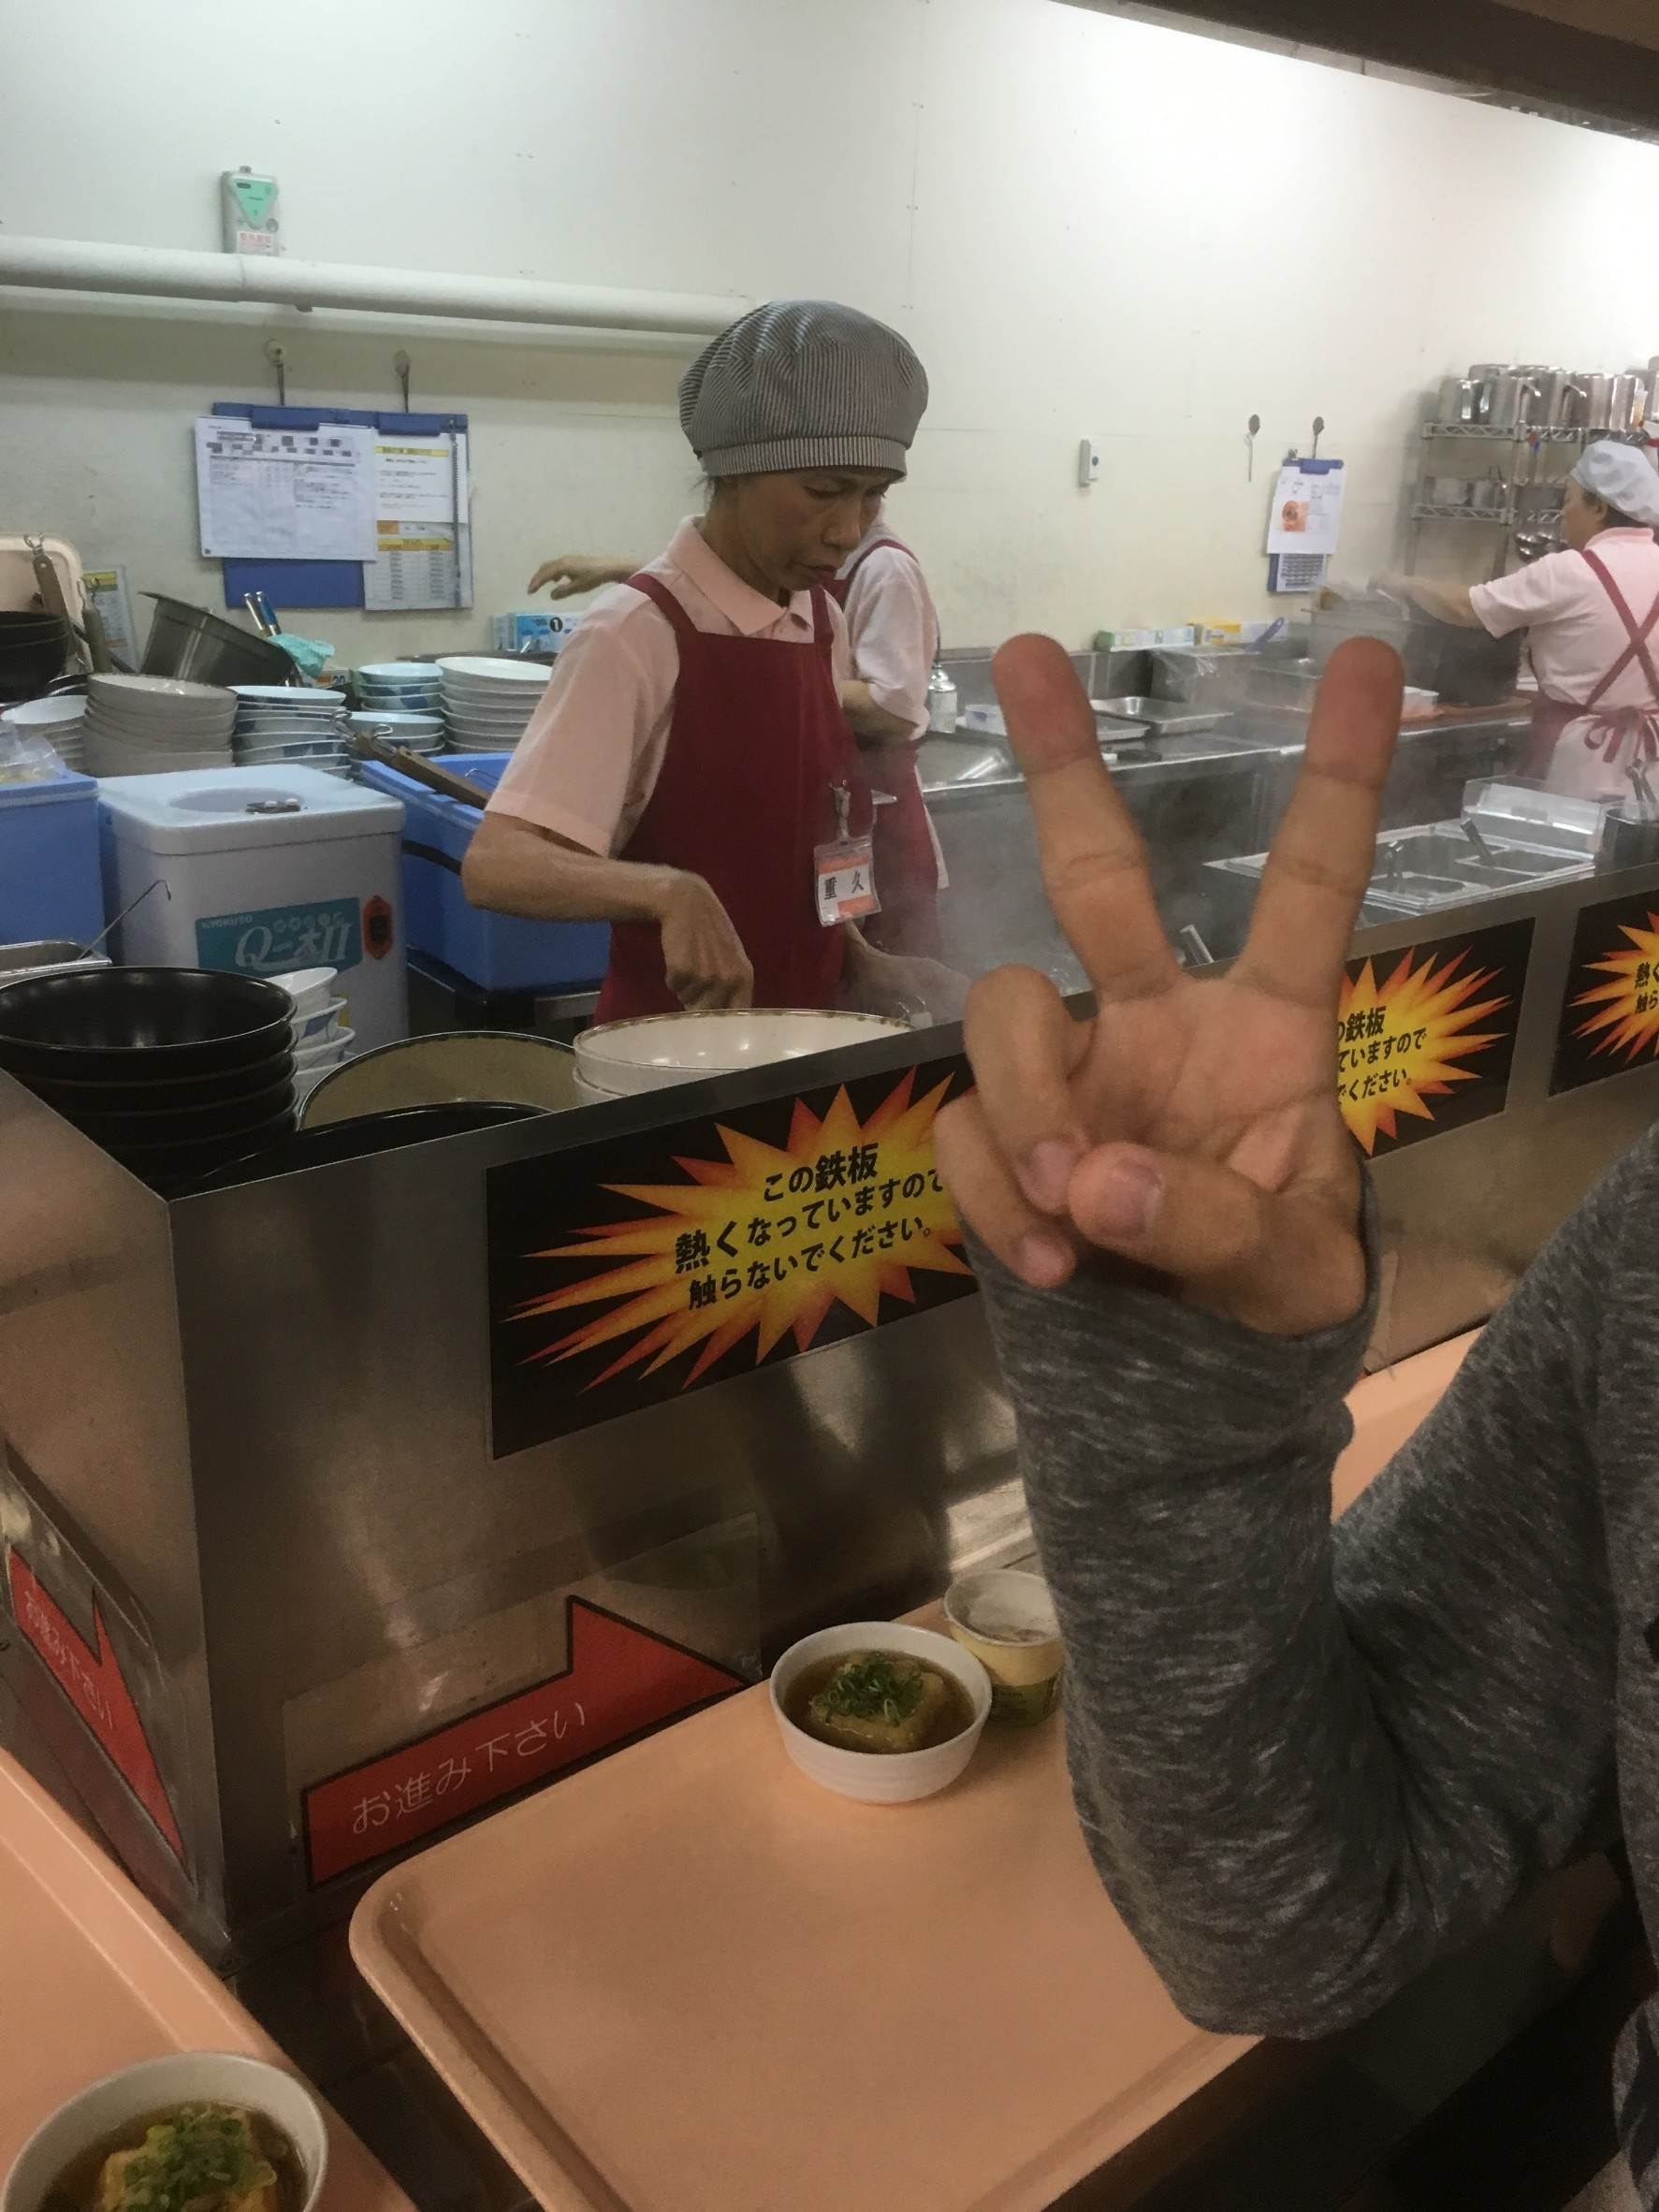
\includegraphics[width=0.5\textwidth]{./section/Shokuji/figures/Shigehisa.jpg}
\caption{LANS Boxで毎日給仕していただいている重久さん。}
\label{Fig:Shigehisa}
\end{figure}
% ----------------------------------------



%%%%%%%%%%%%%%%%%%%%%%%%%%%%%%%
\section{蕎麦は二度美味しい}
%%%%%%%%%%%%%%%%%%%%%%%%%%%%%%%
蕎麦派か、うどん派か。これは議論の分かれる所であり、食べ方や出汁のとり方から何から何まで全く違う日本の誇るべき食べ物である。
俗に関東は蕎麦文化、関西はうどん文化として知られており、時代劇等でも江戸っ子の粋な食べ物として、蕎麦が登場するくらいである。
このように蕎麦は、粋な、いなせな食べ物としてのイメージが定着しており、特に食べ方として次のような作法を取ることが一般的であろう。
\begin{enumerate}
\item つゆに付けず、そのまま味わう
\item 次につゆに付けて、ツルッと味わう
\end{enumerate}
という、いわゆる二度味わうというのが一般的に知られている作法である。
しかし、近年、とある学者が次次に示す、新しい蕎麦の食べ方を考案し、話題になっている。
\begin{enumerate}
\item まず、自分の好みの食べ方で蕎麦を食べきる。
\item 次に、嘔吐する。そうすることで蕎麦が食道を二回通り、同じ値段で蕎麦を二度味わうことができる。
\end{enumerate}
これは非常に画期的な学説であり、+100円で大盛りにするよりも経済的効果も見込める。
たった1200円で、信州そばを二度味わうことができるのである。
しかし、この新手法を用いるには、現在の科学具術では、図\ref{Fig:Soba}に示すように、その副作用が非常に大きく、いかにして簡単に手軽に二度味わうかが次の課題と言えよう。

% ----------------------------------------
\begin{figure}[h]
\centering
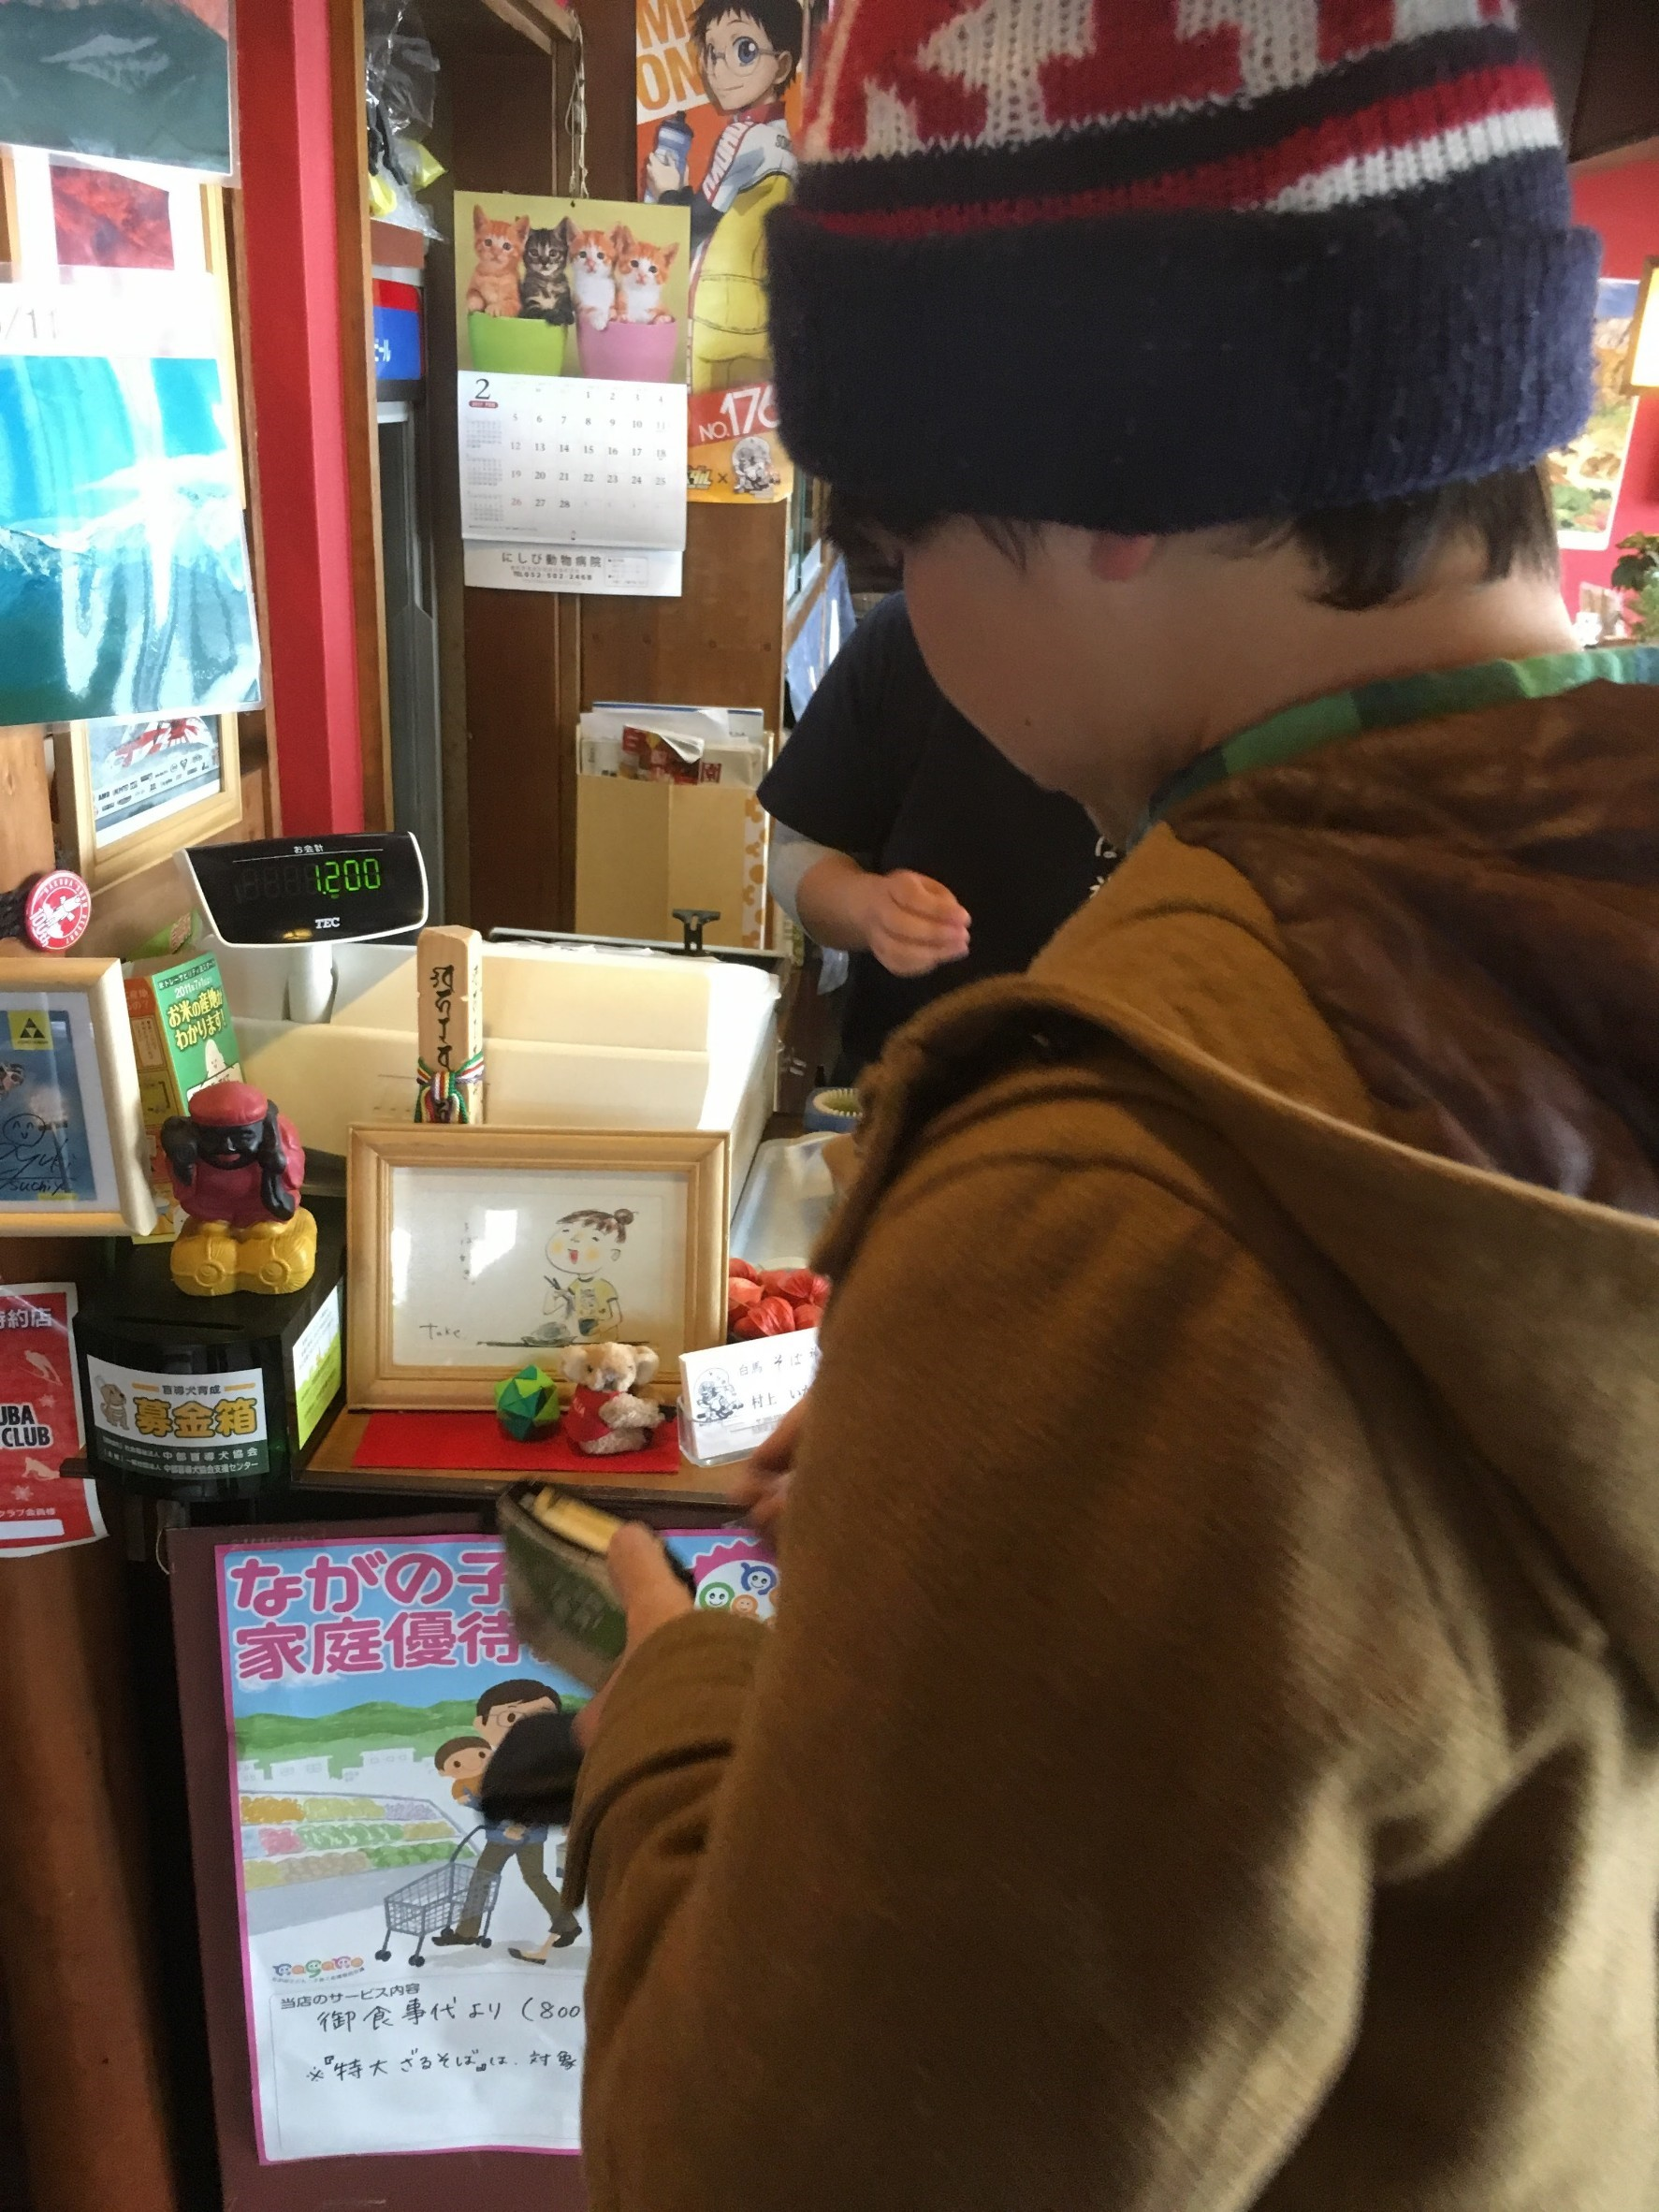
\includegraphics[width=0.4\textwidth]{./section/Shokuji/figures/SobaNido.jpg}

  \caption{開発した新手法を用いて、1200円で二度味わった。どこか誇らしげに財布を取り出し、支払いをする様子が見て取れる。うどん派の言い分として「蕎麦はお腹にたまらず食べた気がしない」との主張があるが、この新手法を用いれば、そのような主張は一蹴することができよう。}
\label{Fig:SobaNido}
\end{figure}
% ----------------------------------------



% ----------------------------------------
\begin{figure}[h]
\centering
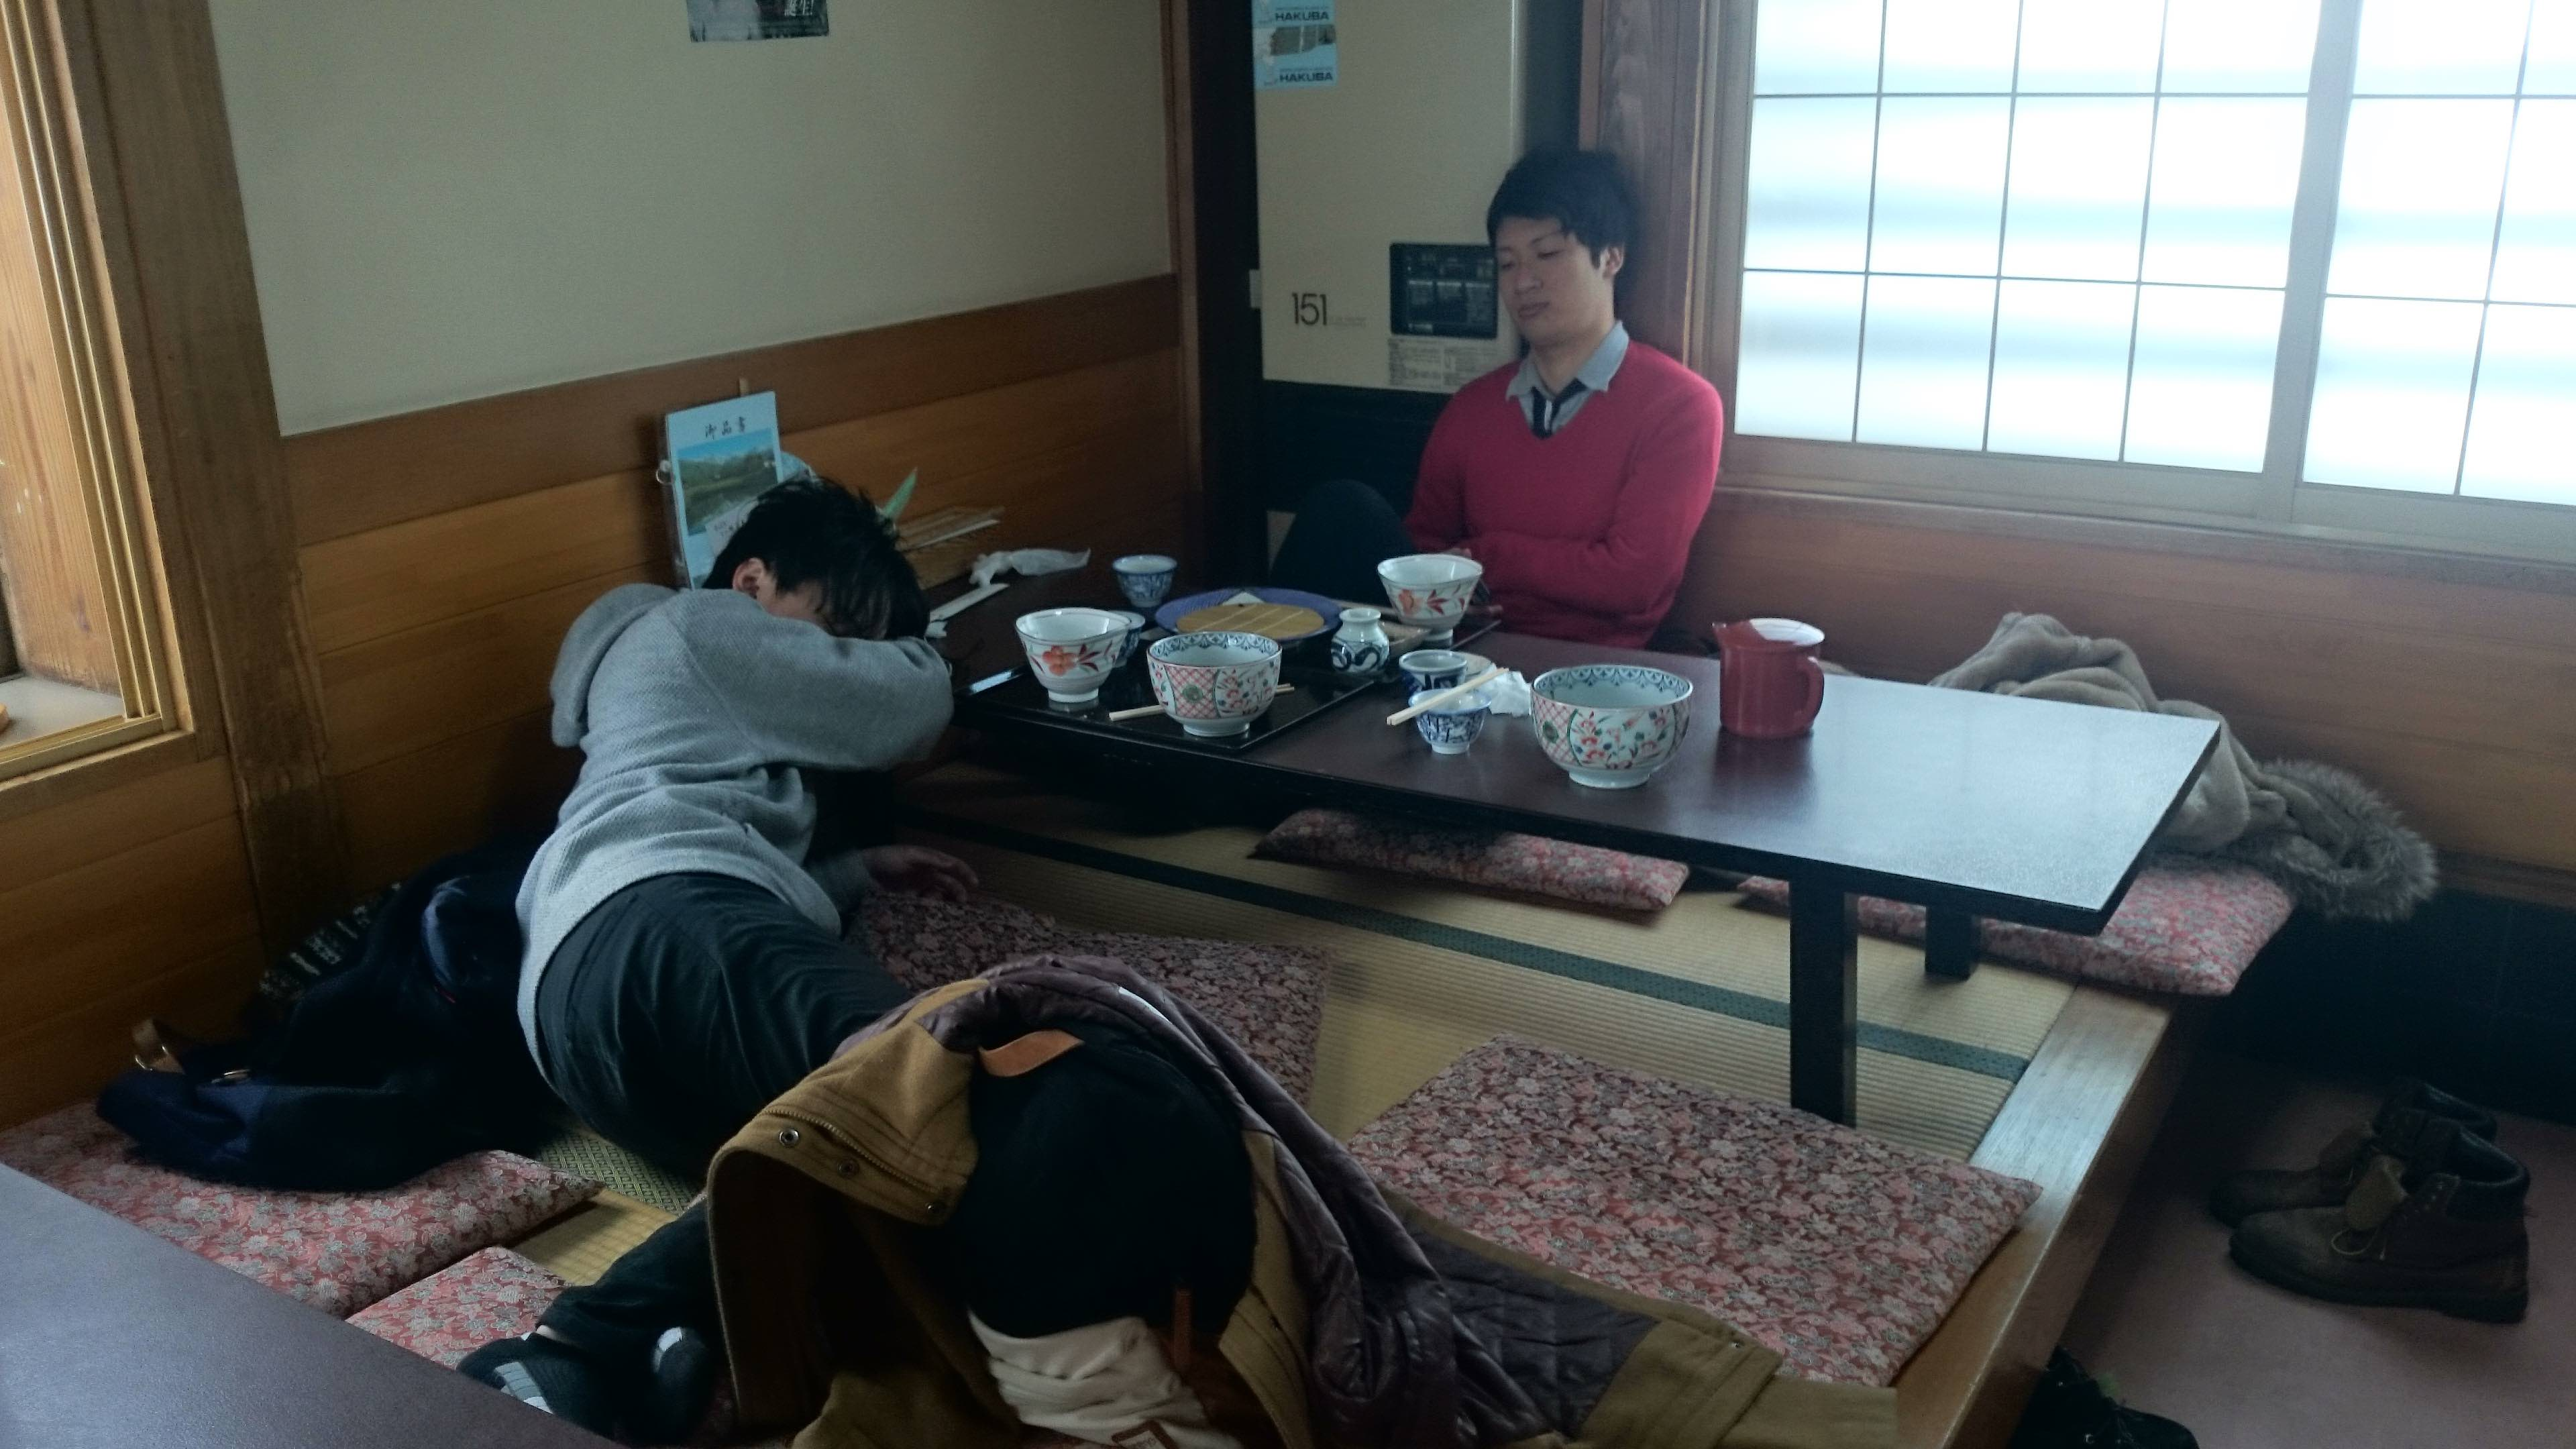
\includegraphics[width=0.6\textwidth]{./section/Shokuji/figures/Soba.jpg}
  \caption{副作用により、死人と化した。}
\label{Fig:Shigehisa}
\end{figure}
% ----------------------------------------

%%%%%%%%%%%%%%%%%%%%%%%%%%%%%%%
\section{自炊生活フロンティア}
%%%%%%%%%%%%%%%%%%%%%%%%%%%%%%%
最近は世知辛い世の中であり、いかにアベノミクスで日本経済が持ち直ったといえど、庶民の生活の改善には程遠いのが現状である。
そのため、世のサラリーマンを始め、学生も極力出費を抑えるため、自炊してお弁当を持ってくることが多いと言われている。
日本人といえば、白米であり、お弁当を作る際には白米と、何か簡単なおかずさえ作ってしまえば、一応お弁当の体裁は整えることができる。
しかし、おかずを作るのにも、数百円はかかっており、もちろん外食するより格段に安いため出費を抑えることができるが、自炊フロンティア(もしくは自炊生活末期症状)では、おかず作成に数百円を費やすことでさえ億劫に感じられているのが現状である。
そこで、自炊フロンティアでは、おかずとして駄菓子のわさびのり、蒲焼さん太郎、酢だこさん太郎をチョイスすることにより、一食にかかる費用を概算で約10分の1以下に大きく削減することが出来たのである。
% ----------------------------------------
\begin{figure}[h]
\centering
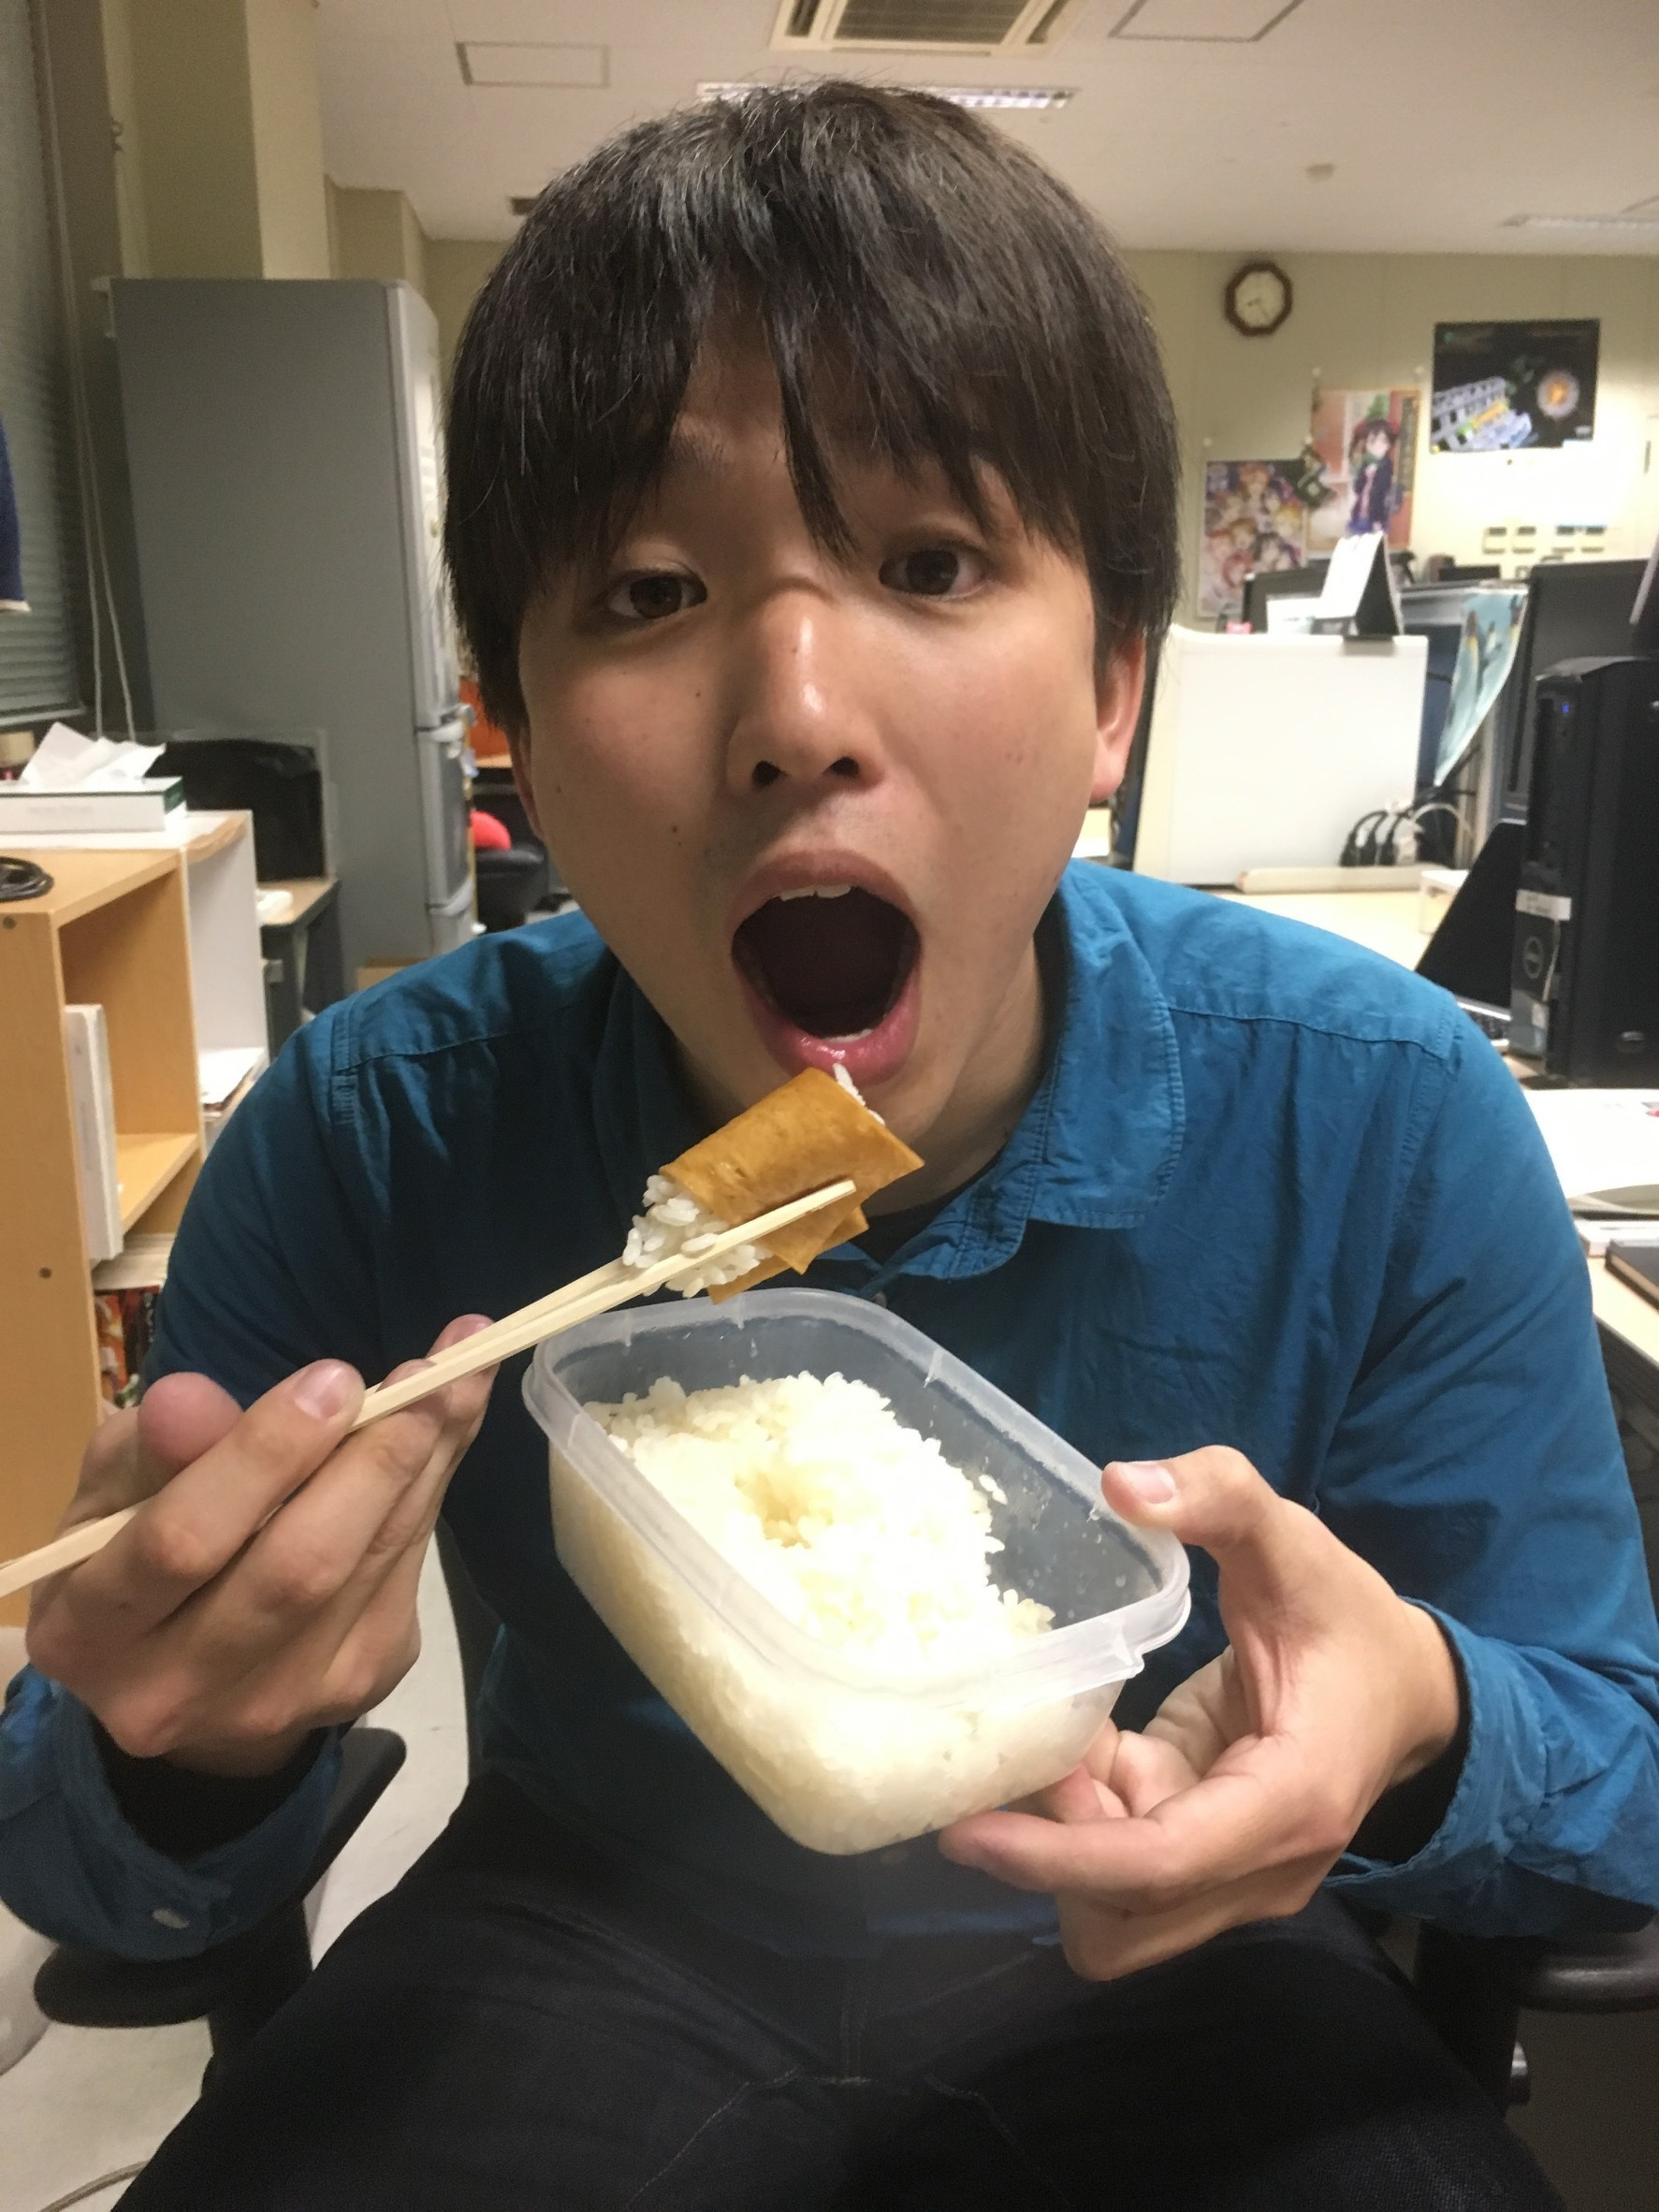
\includegraphics[width=0.4\textwidth]{./section/Shokuji/figures/JisuiMakki.jpg}
  \caption{流行りの弁当男子。持参した白米と、セブンイレブンで購入した駄菓子との最強コラボで晩ごはんを耐えしのぐ、涙ぐましい学生の姿である。小学生の頃は、蒲焼さん太郎ひとつ取っても、非常に心躍るものであったが、それから10数年たった今では、駄菓子とはこれほどまでに虚しいものであるのか、と改めて実感した。}
\label{Fig:Shigehisa}
\end{figure}
% ----------------------------------------


%%%%%%%%%%%%%%%%%%%%%%%%%%%%%%%
\section{アブラ足りてますか?}
%%%%%%%%%%%%%%%%%%%%%%%%%%%%%%%
「アブラ足りてますか足りてますか?」に対して「充分に足りている」と答えた場合、それは重症患者であろう。
一般人にとって、アブラとは食事の際にしか触れない概念であるが、重症患者の場合、食事の枠を飛び越え、日常的にアブラに接しているのである。
一年の計は元旦にあり、という有名なことわざを拝借するなら、重症患者にとって「一日の挨拶はアブラにあり」であろう。
すれ違う際、何かを叫ぶ際、熱いものに触ってしまった際、等で重症患者は「アブラ」を口にしてしまう。


% ----------------------------------------
\begin{figure}[h]
\centering
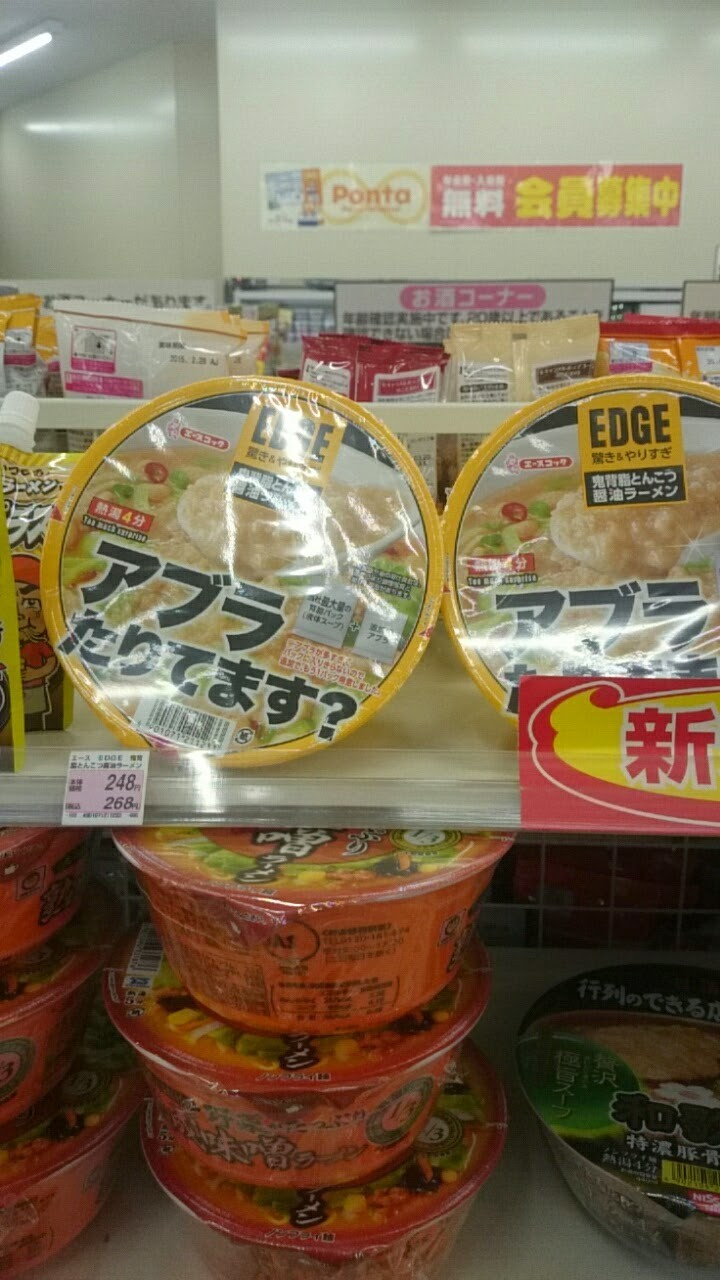
\includegraphics[width=0.4\textwidth]{./section/Shokuji/figures/AburaTaritemasuka.jpg}
  \caption{十二分にアブラは足りている。しかし、現代人にはアブラは不足していると言えよう。}
\label{Fig:Shigehisa}
\end{figure}
% ----------------------------------------

%%%%%%%%%%%%%%%%%%%%%%%%%%%%%%%
\section{リプトンタワー}
%%%%%%%%%%%%%%%%%%%%%%%%%%%%%%%
食事をより楽しくするものとして、西洋では食中酒という文化が広く知られている。
日本でも食事に合う酒、その中でも魚介類に会う酒、肉類に会う酒、などなど非常に幅広く食中酒が普及している。
その中で、食中を超え、いついかなるときでもリプトンと、いついかなる時でも烏龍茶を飲み続けた男たちがいることを、皆さんは御存知だろうか?
彼らは、食事以外でも暇を見つけてはリプトン・烏龍茶を飲み続けたのである。
ではなぜ彼らは、このような偉業を達成できたのであろうか?それは一つの小さな不満に端を発しているのである。

%==========================%
\subsection{引き出しという概念}
%==========================%
彼らが配属された研究室は、平たく言えば、席の当たり外れが非常に大きかった。
その不公平姓は席の位置に始まり、本来であれば一人一個分配される移動式引き出しがないデスクも存在したのである。
席の位置は、例えば図書館にこもったりすれば特に不満を感じないが、備品に関する不公平性は、その備品が分配されない限り解消されないのである。
確かに、近年は科研費の縮小や国家予算の再分配に伴い、備品にかける金額も限られてくるのが現状である。
特に配属されたての4回生への備品など、最もプライオリティの低いものであることは認めざるを得ない。
しかし、移動式引き出しの有無は、実行的なデスクの拡張、教科書置き場、として使うことができ、作業効率に関わってくるところである。
そこで、彼らは、なんとかしてこの移動式引き出しを自分たちで用意できないかと、その方法を模索していたのである。

%==========================%
\subsection{リサイクルという概念}
%==========================%
そんななか$1L$リプトンを飲んでいた男が、ひらめいたのである。
科学史において、ひらめきとは重要であり、エジソンも「ひらめきはナンチャラ」と言っていたくらいなので、非常に重要である。
かの有名なベンゼン環を発見したベンゼン氏は、睡眠している最中に蛇が自らのしっぽをかみ、輪になっている光景を見たことに閃き、それまででは考えられていなかった輪になっている化学構造を思いついたのである。
おそらく、これは推論であるが、リプトンからの閃きも寝ている最中に、はたと気づき「この空き容器を集めれば、簡単に引き出しが作れるのではないか?」と思いついたのであろう。
さらに、空き容器とは本来ゴミであり、リサイクルの観点からも非常に好感の持てる発想であり、人類の英知とも言えよう。
その動きに呼応するように、「私は烏龍茶で援助する」と名乗りをあげた人物がおり、彼ら二人をもってここに移動式リプトン・烏龍茶型引き出しの作成が始まったのである。

%==========================%
\subsection{積んでおくという概念}
%==========================%
しかし、引き出し建設には、非常に多くの空き容器が必要であることが、当時の試算でわかっており、
建設に必要な本数が集まるまで、5本一組の構造体にして積み上げる形で保存しておくこととなった。
一段、また一段と積み上がっていく度に達成感を感じ、次第に当初の目標であった引き出し作成よりも、天井まで届くタワーの建設へと目的がシフトしていった。
図\ref{Fig:LiptonTower_tochuu}に示すように、建設途中のリプトンタワーはある程度の高さまでいくと、不安定になるため、天井との間に突っ張り棒を敷いて耐震補強していたことが分かる。
また、その突っ張り棒には、その時に1年遅れくらいでハマっていた「あまちゃん」の主演女優の能年玲奈の写真が飾られている。

このタワーの色味からも分かるように、当初はリプトンから始まった建設であるが、一人の烏龍茶界の天才により、タワー構成の半分以上が烏龍茶となっていることが見て取れる。
この烏龍茶の成長率は、タワー建設計画終了まで持続されることとなる。
ここまでに、リプトンと烏龍茶の構成率の違いが現れた原因として、値段が1.5倍違うことが挙げられよう。
リプトンは150円ほどであり、烏龍茶の方が安いのである。
また、健康面からも一日に何本もリプトンを飲むことはあまり好ましくなく、その点、烏龍茶は何本飲んでもなんとなく大丈夫であるとの観点から、構成率に大きな差を生んでいる。
さらにその構成率の違いに拍車をかける決定打は、リプトンのリニューアルである。
従来のパッケージを新しいものに置き換えたところまではよかったのであるが、なんと内容量もリニューアルされ、従来の1リットルから950ミリリットルへと削減されたのである。
このことから、リプトンを買うコスパの悪さが構成率の違いを生み出したと言っても過言ではない。


% ----------------------------------------
\begin{figure}[h]
\centering
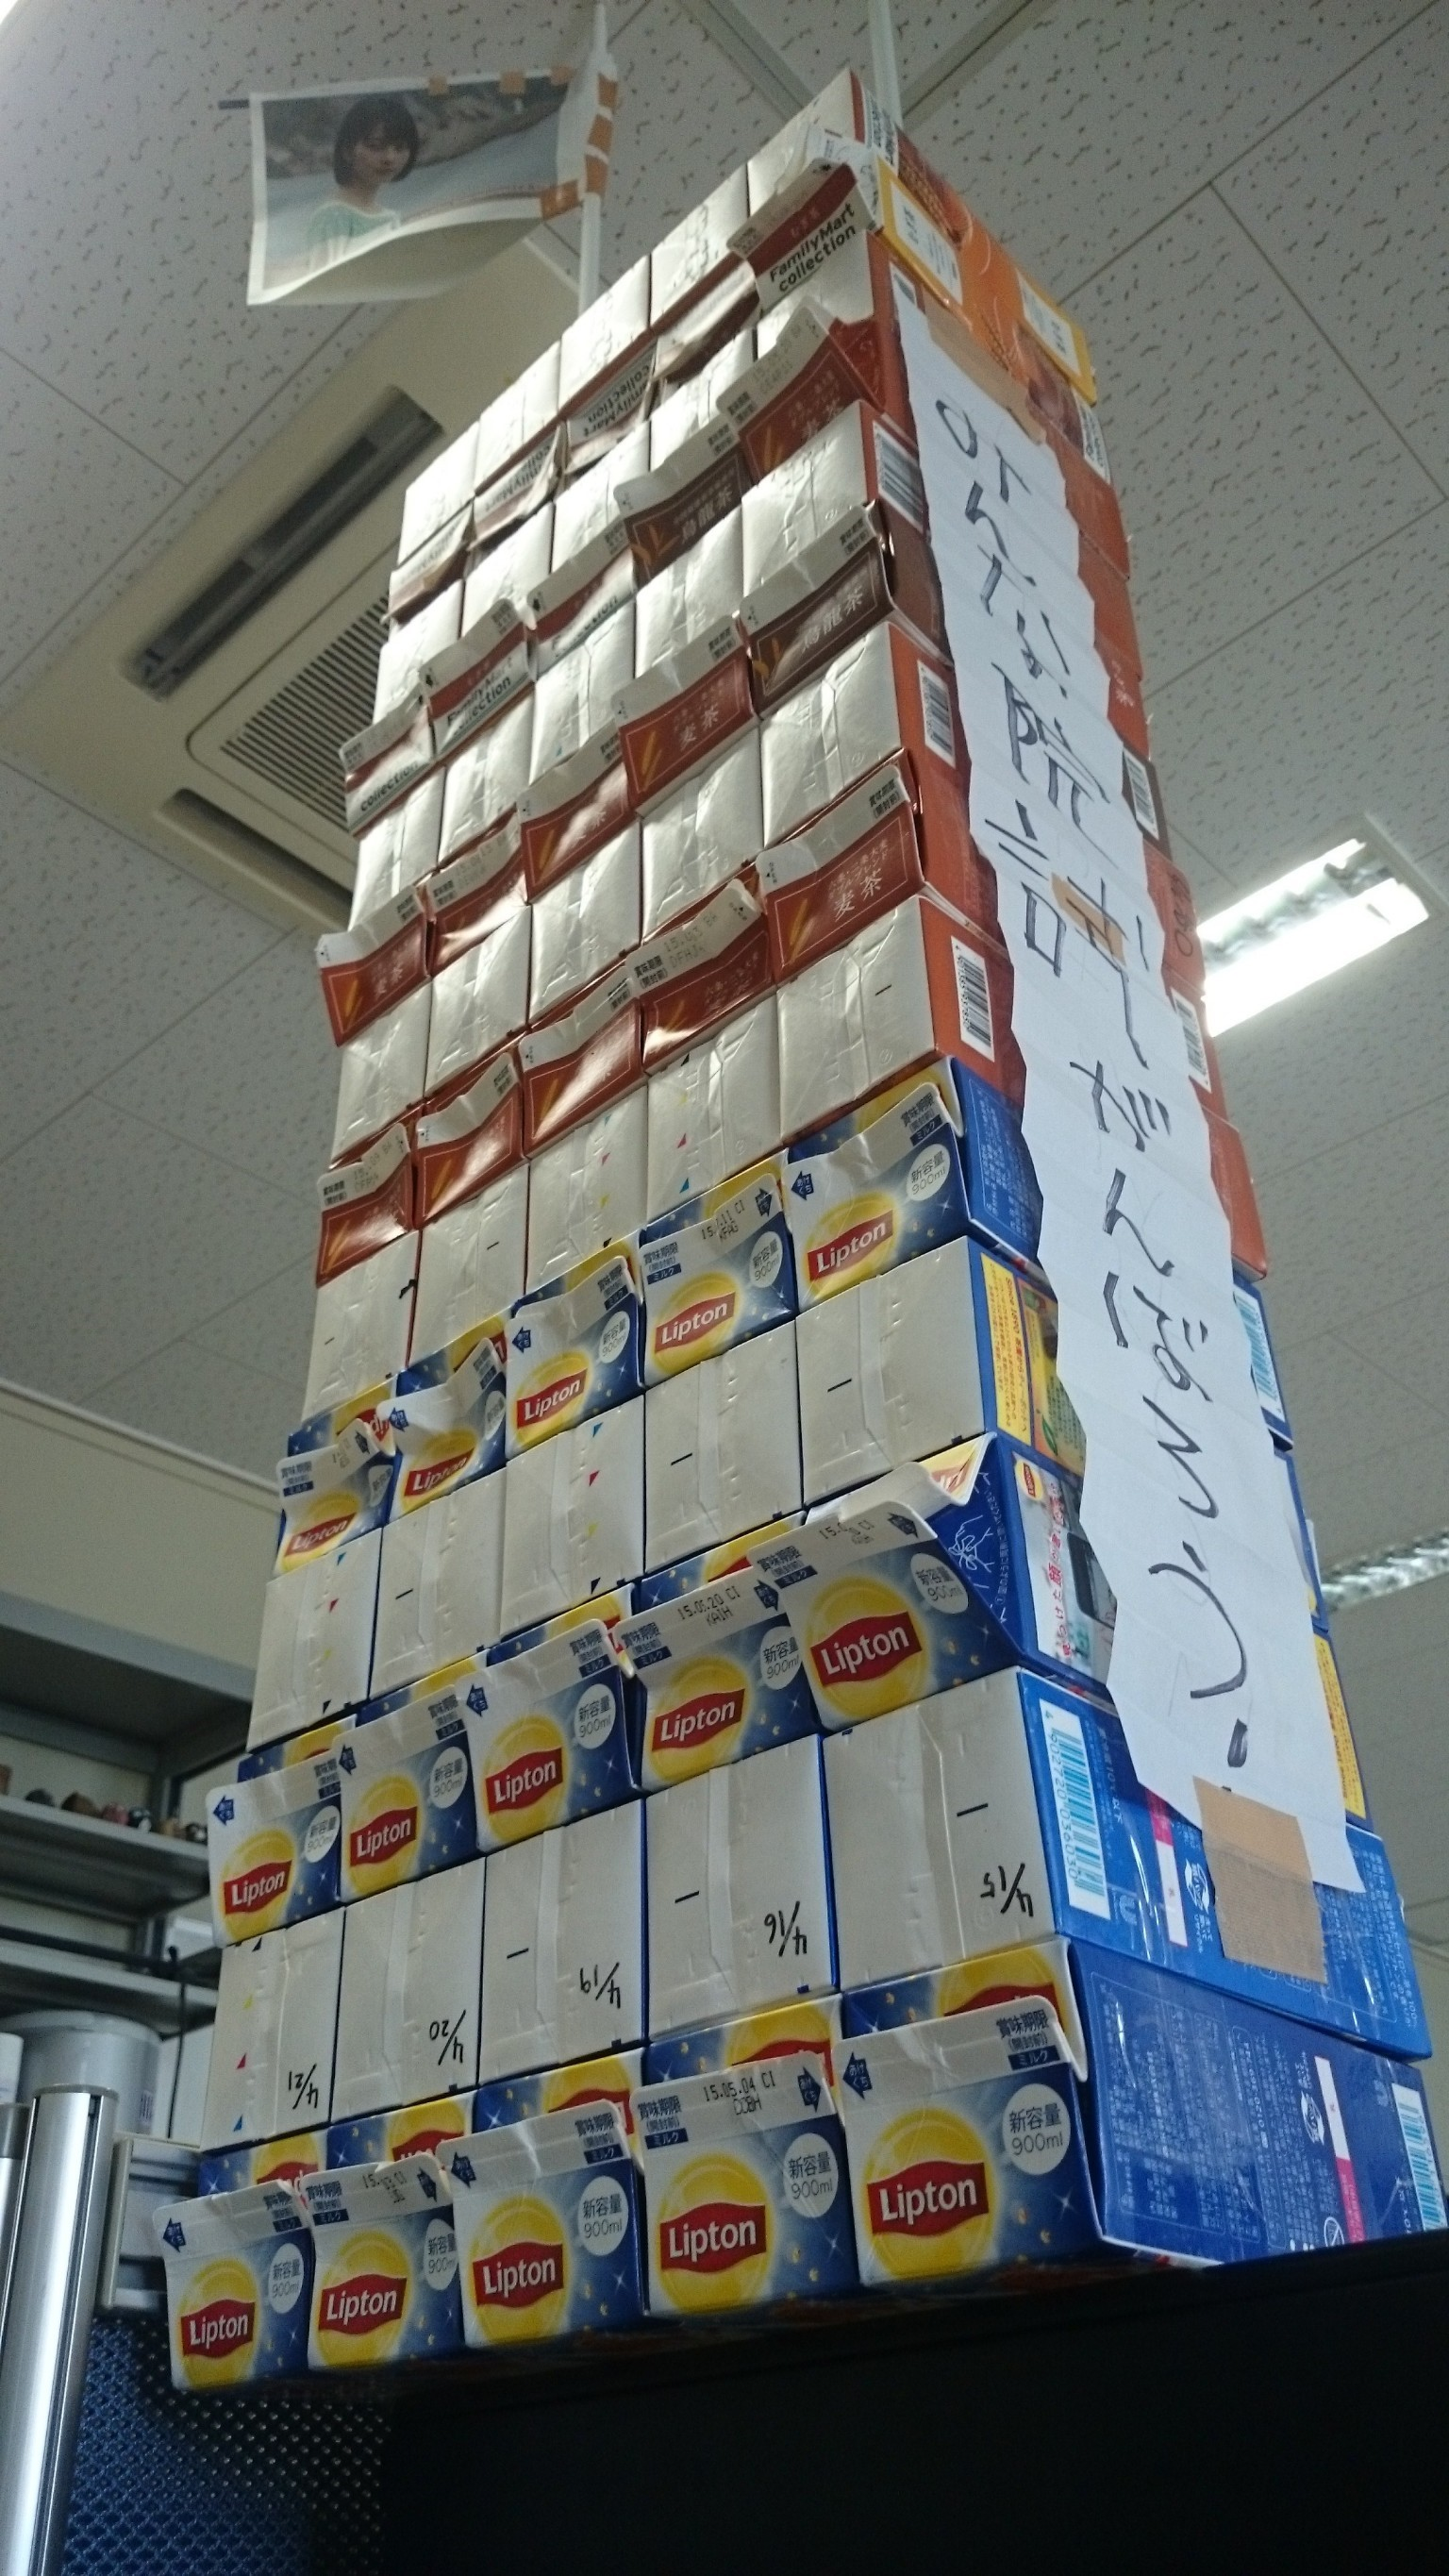
\includegraphics[width=0.4\textwidth]{./section/Shokuji/figures/LiptonTower_tochuu.jpg}
  \caption{引き出し作成のための建材を保管している様子。「みんな院試がんばろう!」と書かれた横断幕が貼られていることからも、この建材置き場は、学生の交流の場として活かされていたことも分かる。}
\label{Fig:LiptonTower_tochuu}
\end{figure}
% ----------------------------------------

%==========================%
\subsection{風邪なのに飲み続けるという概念}
%==========================%
リプトンマンをさしおいて、烏龍茶男は雨の日も風の日も、風邪の日も烏龍茶を飲み続けた。
どれだけ咳き込んでいようとも、烏龍茶を飲んで喉を冷やし続け、風邪を悪化させ続けた。
このように涙ぐましい努力も、構成に語り継いでいくべきであろう。

%==========================%
\subsection{高さ調整のために電磁力学の教科書を使うという概念}
%==========================%
ようやく努力の成果が結実するときがきた。
タワー完成である。
しかし、デスクトップPCと天井との間には数cmの隙間が出来てしまうことがわかったのだ。
そこで機転を利かせ、電磁力学の教科書を挟んでおくことにした。
後に藏重教授から「そんなことしてるから電磁気の点数がアハアハアハ」となじられるのである。

% ----------------------------------------
\begin{figure}[h]
\centering
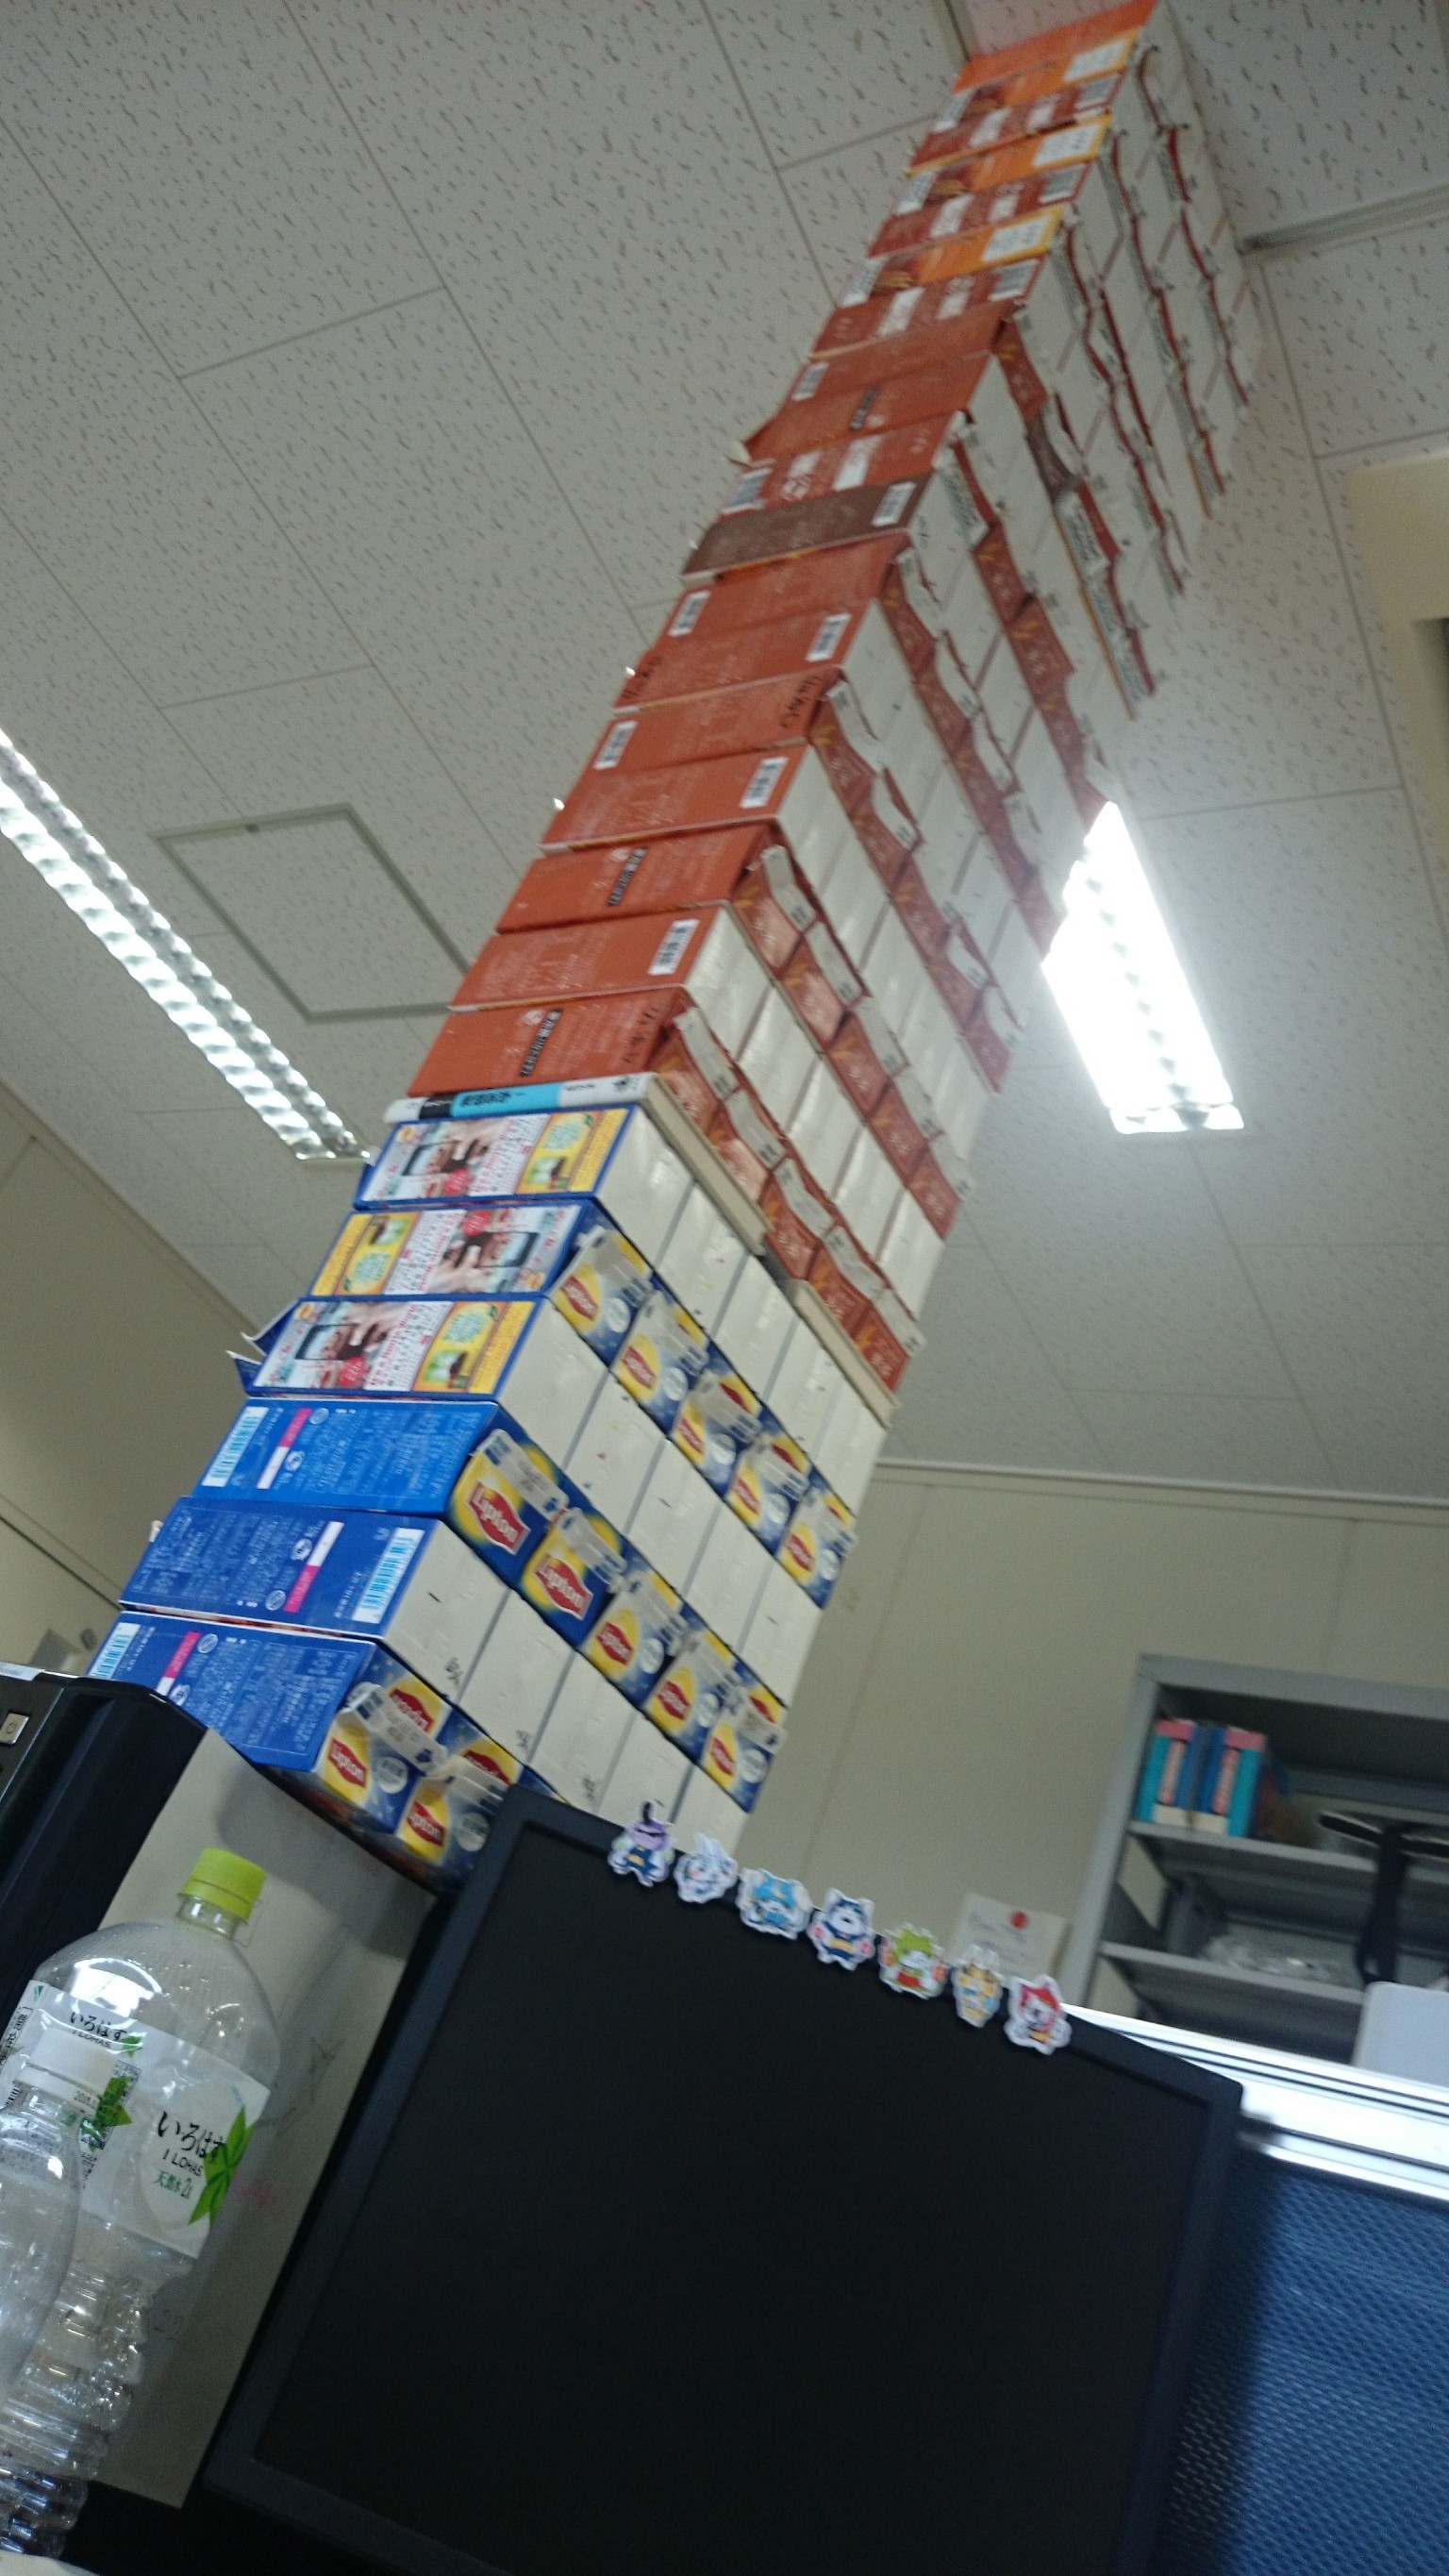
\includegraphics[width=0.4\textwidth]{./section/Shokuji/figures/LiptonTower_final.jpg}
  \caption{見事なタワーである。もはや色合いとしては、烏龍茶タワーと呼ぶべきかもしれない。建設後半タケダ氏は、烏龍茶の追い上げに度肝を抜かし、お茶飲みとしての才能に限界を感じ一線から退いたのである。ちなみに、このタワーの建設費用は概算で13500円である。}
\label{Fig:LiptonTower_final}
\end{figure}
% ----------------------------------------



%==========================%
\subsection{実は邪魔だったという概念}
%==========================%
このリプトンタワー、建設者からの視点では、特に問題なく積み上がっていたのであるが、それとは対照的に近隣住民の一声で計画が頓挫、建設企業の廃業にまで追い込まれたのである。\par
「この柱のせいで時計が見えへんから、捨ててこい」\par
なるほど、と感じた反面、別にええやろ、と感じたのは言うまでもない。


%%%%%%%%%%%%%%%%%%%%%%%%%%%%%%%
\section{日本人の精神}
%%%%%%%%%%%%%%%%%%%%%%%%%%%%%%%

% ----------------------------------------
\begin{figure}[h]
\centering
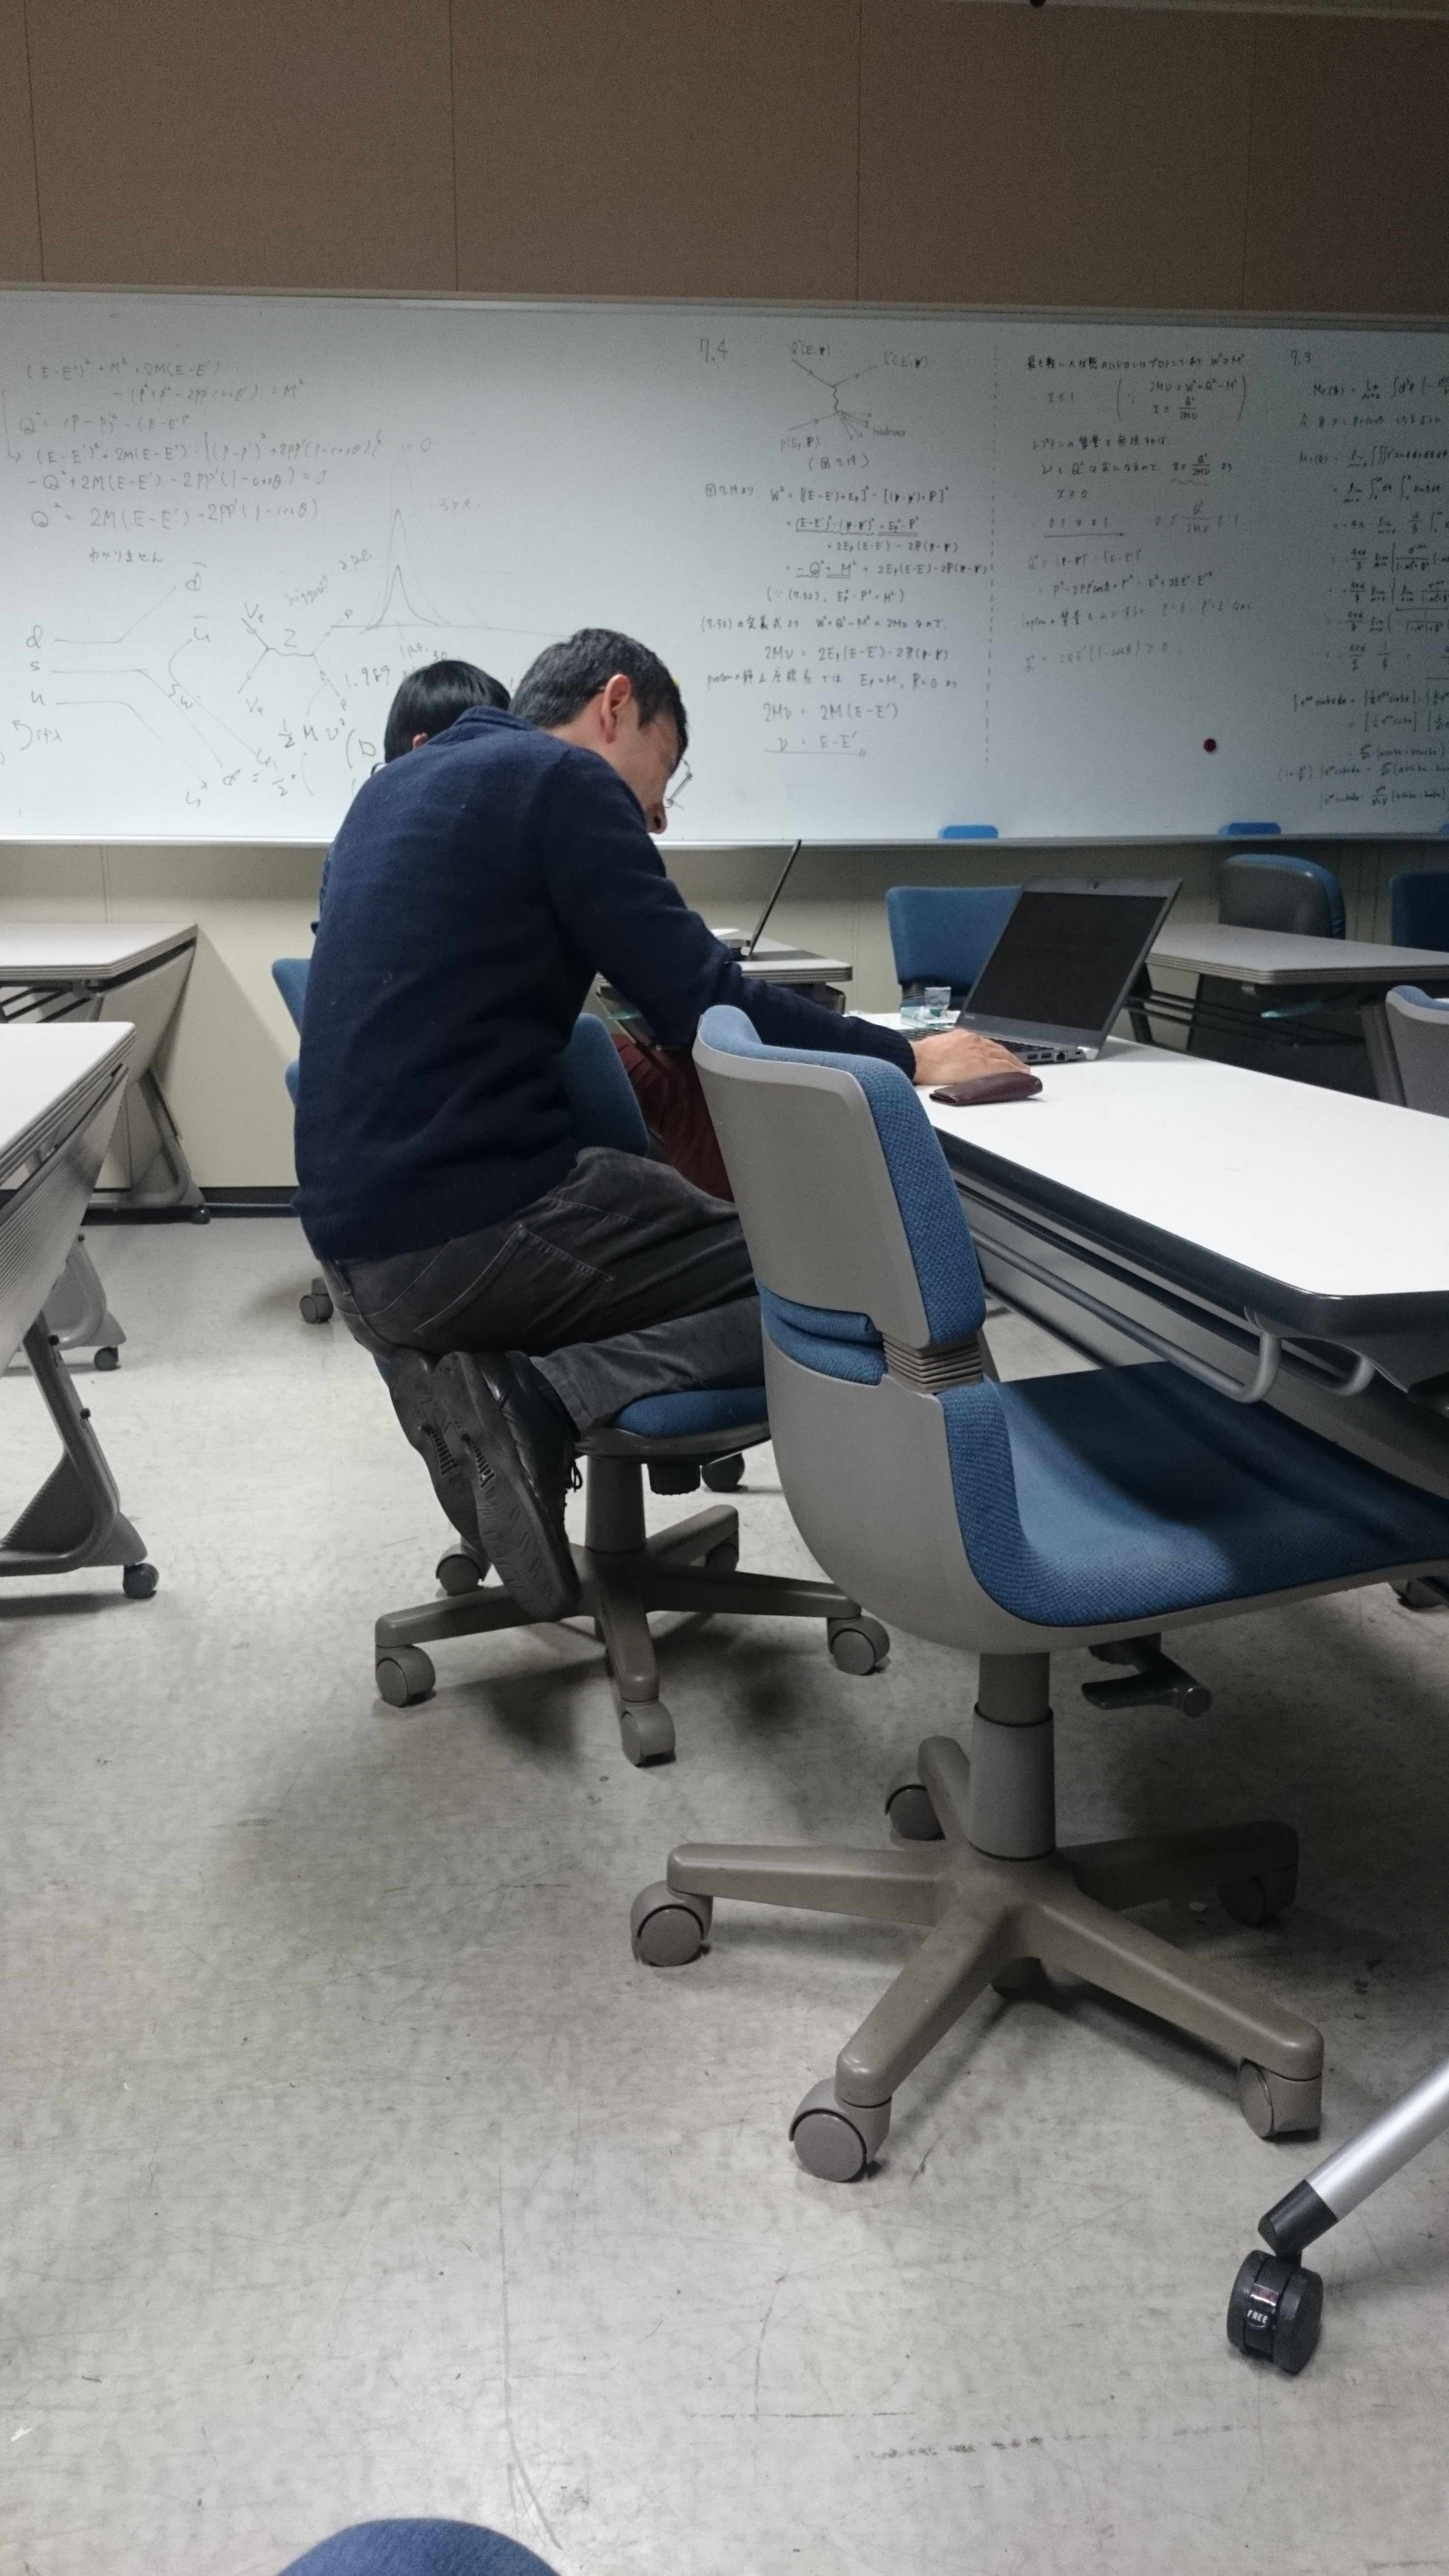
\includegraphics[width=0.4\textwidth]{./section/Shokuji/figures/Seiza.jpg}
  \caption{いかなるときも日本人の心を忘れず、椅子に座りつつ正座を行う}
\label{Fig:Seiza}
\end{figure}
% ----------------------------------------



%%%%%%%%%%%%%%%%%%%%%%%%%%%%%%%
\section{おばコーヒー}
%%%%%%%%%%%%%%%%%%%%%%%%%%%%%%%
世の中にはその人の名を冠した地名や建物などが多く見受けられる。
しかし、コーヒーにその名を残した偉人が未だかつて存在しただろうか?
現代に伝わる七不思議の一つ、それが「おばコーヒー」である。
このおばコーヒーというのは、生協オリジナルの上質なコーヒー牛乳であり、200mLしか入っていないのに100円するという、穿った見方をすればボッタクリのような商品であるが、消費者を魅了してやまないのは、その独特の飲み方のスタイルにある。
普通に一般の方が飲むと、吸い終わった後に容器に空気が入る音で「ジュボッ」という音がする。
この飲み方では、そう、授業中には迷惑になって飲めないのである。
しかし、この飲み方に一石を投じた人間がおり、それが「おば」である。
このおば氏は、吸い終わった後、容器の中に空気が戻ることが原因で音がなるので、最初から飲む時に容器を押さえつけてなるべく空気の出戻りを少なくすれば消音できると提案した。
画期的な発見であることにその当時の学者は誰一人気づかなかったが、これが後に世界的に受け入れられ、開発したおば氏の名を冠し、「おばコーヒー」と一部の学者から呼ばれるようになったのである。

% ----------------------------------------
\begin{figure}[h]
\centering
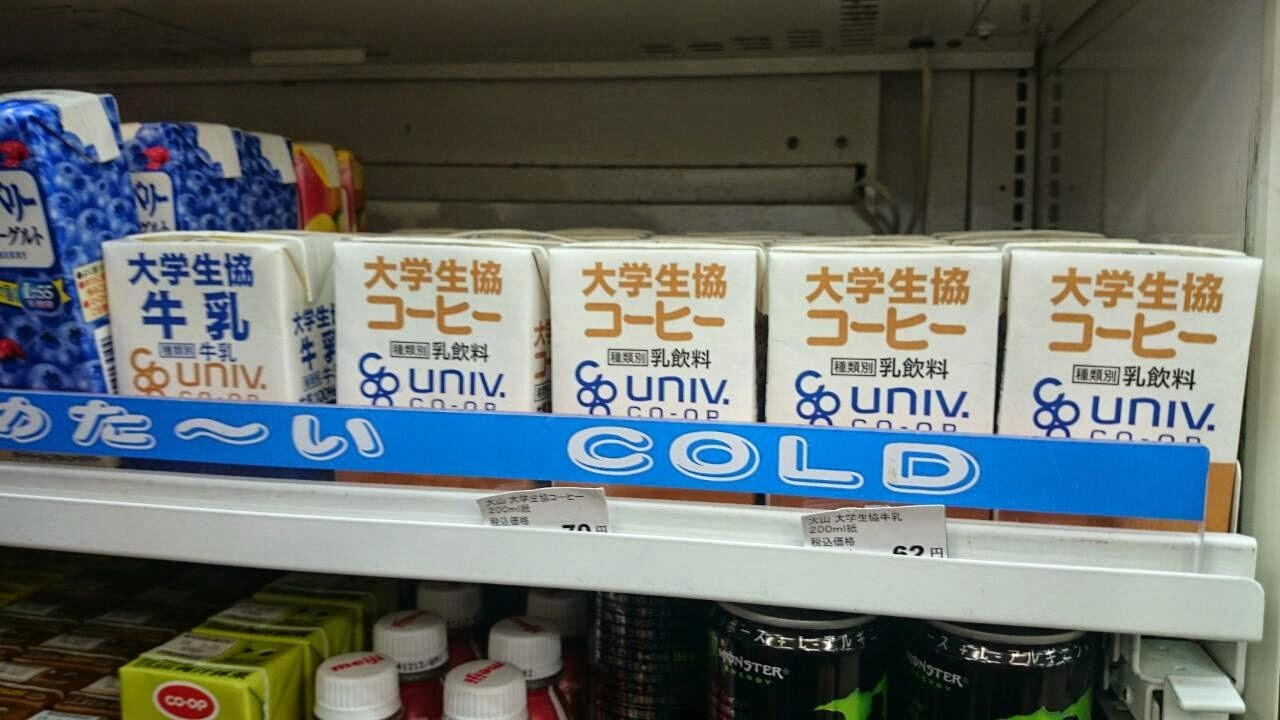
\includegraphics[width=0.4\textwidth]{./section/Shokuji/figures/ObaCoffee.jpg}
  \caption{生協で売上トップをひた走る人気商品であればうれしいが、、、。見て分かるように、牛乳よりも多く展開されている商品である。ちなみにこの牛乳に関して、オガワ氏が飲み会の前に度々飲み「牛乳で胃袋に膜を張ってアルコール吸収率をうんぬんかんぬん」と言っていたが、その効果のほどは本人以外分からない。個人的には、牛乳飲んでも、ウコン飲んでも、死ぬときは死ぬ。}
\label{Fig:Seiza}
\end{figure}
% ----------------------------------------

%%%%%%%%%%%%%%%%%%%%%%%%%%%%%%%
\section{夕食の範疇を超越する}
%%%%%%%%%%%%%%%%%%%%%%%%%%%%%%%
原動機付自転車で神戸の街を颯爽と駆け巡る若者にとって、徒歩で数十分かかる場所へもラクラクとアクセスできるので、非常に行動範囲が広がる。
しかし、良い事ばかりではない。「お腹すいた」と思ったらすぐにどこかへ行けてしまう怖さも秘めているのである。
原動機付自転車に乗れば日頃の運動量が減るばかりではなく、ガソリンを使い脂肪を蓄えるため、様々な場所へ移動することになるのだ。


%==========================%
\subsection{すき家}
%==========================%
夜食とは、夕食を食べた後に小腹がすいてしまい、スナック菓子などに手が伸びてしまうことを言う。
では、夕食を食べずバイトが22時過ぎに終わり、お腹が空いてしまった場合はどうすればいいのだろうか?
その答えは近所のすき家に駆け込む、である。
何ご飯なのだろうか?と聞かれても、晩御飯の概念を超越しており、ただただ健康を害するだけである。
しかし彼らは20代も前半であり、まだまだ新陳代謝の衰えは感じていなかったのであろう。
「若い頃にむちゃするんじゃなかった」と思ってももう遅い、とキートン山田に突っ込まれそうである。

\begin{figure}[htbp]
% \begin{minipage}{0.5\hsize}
\centering
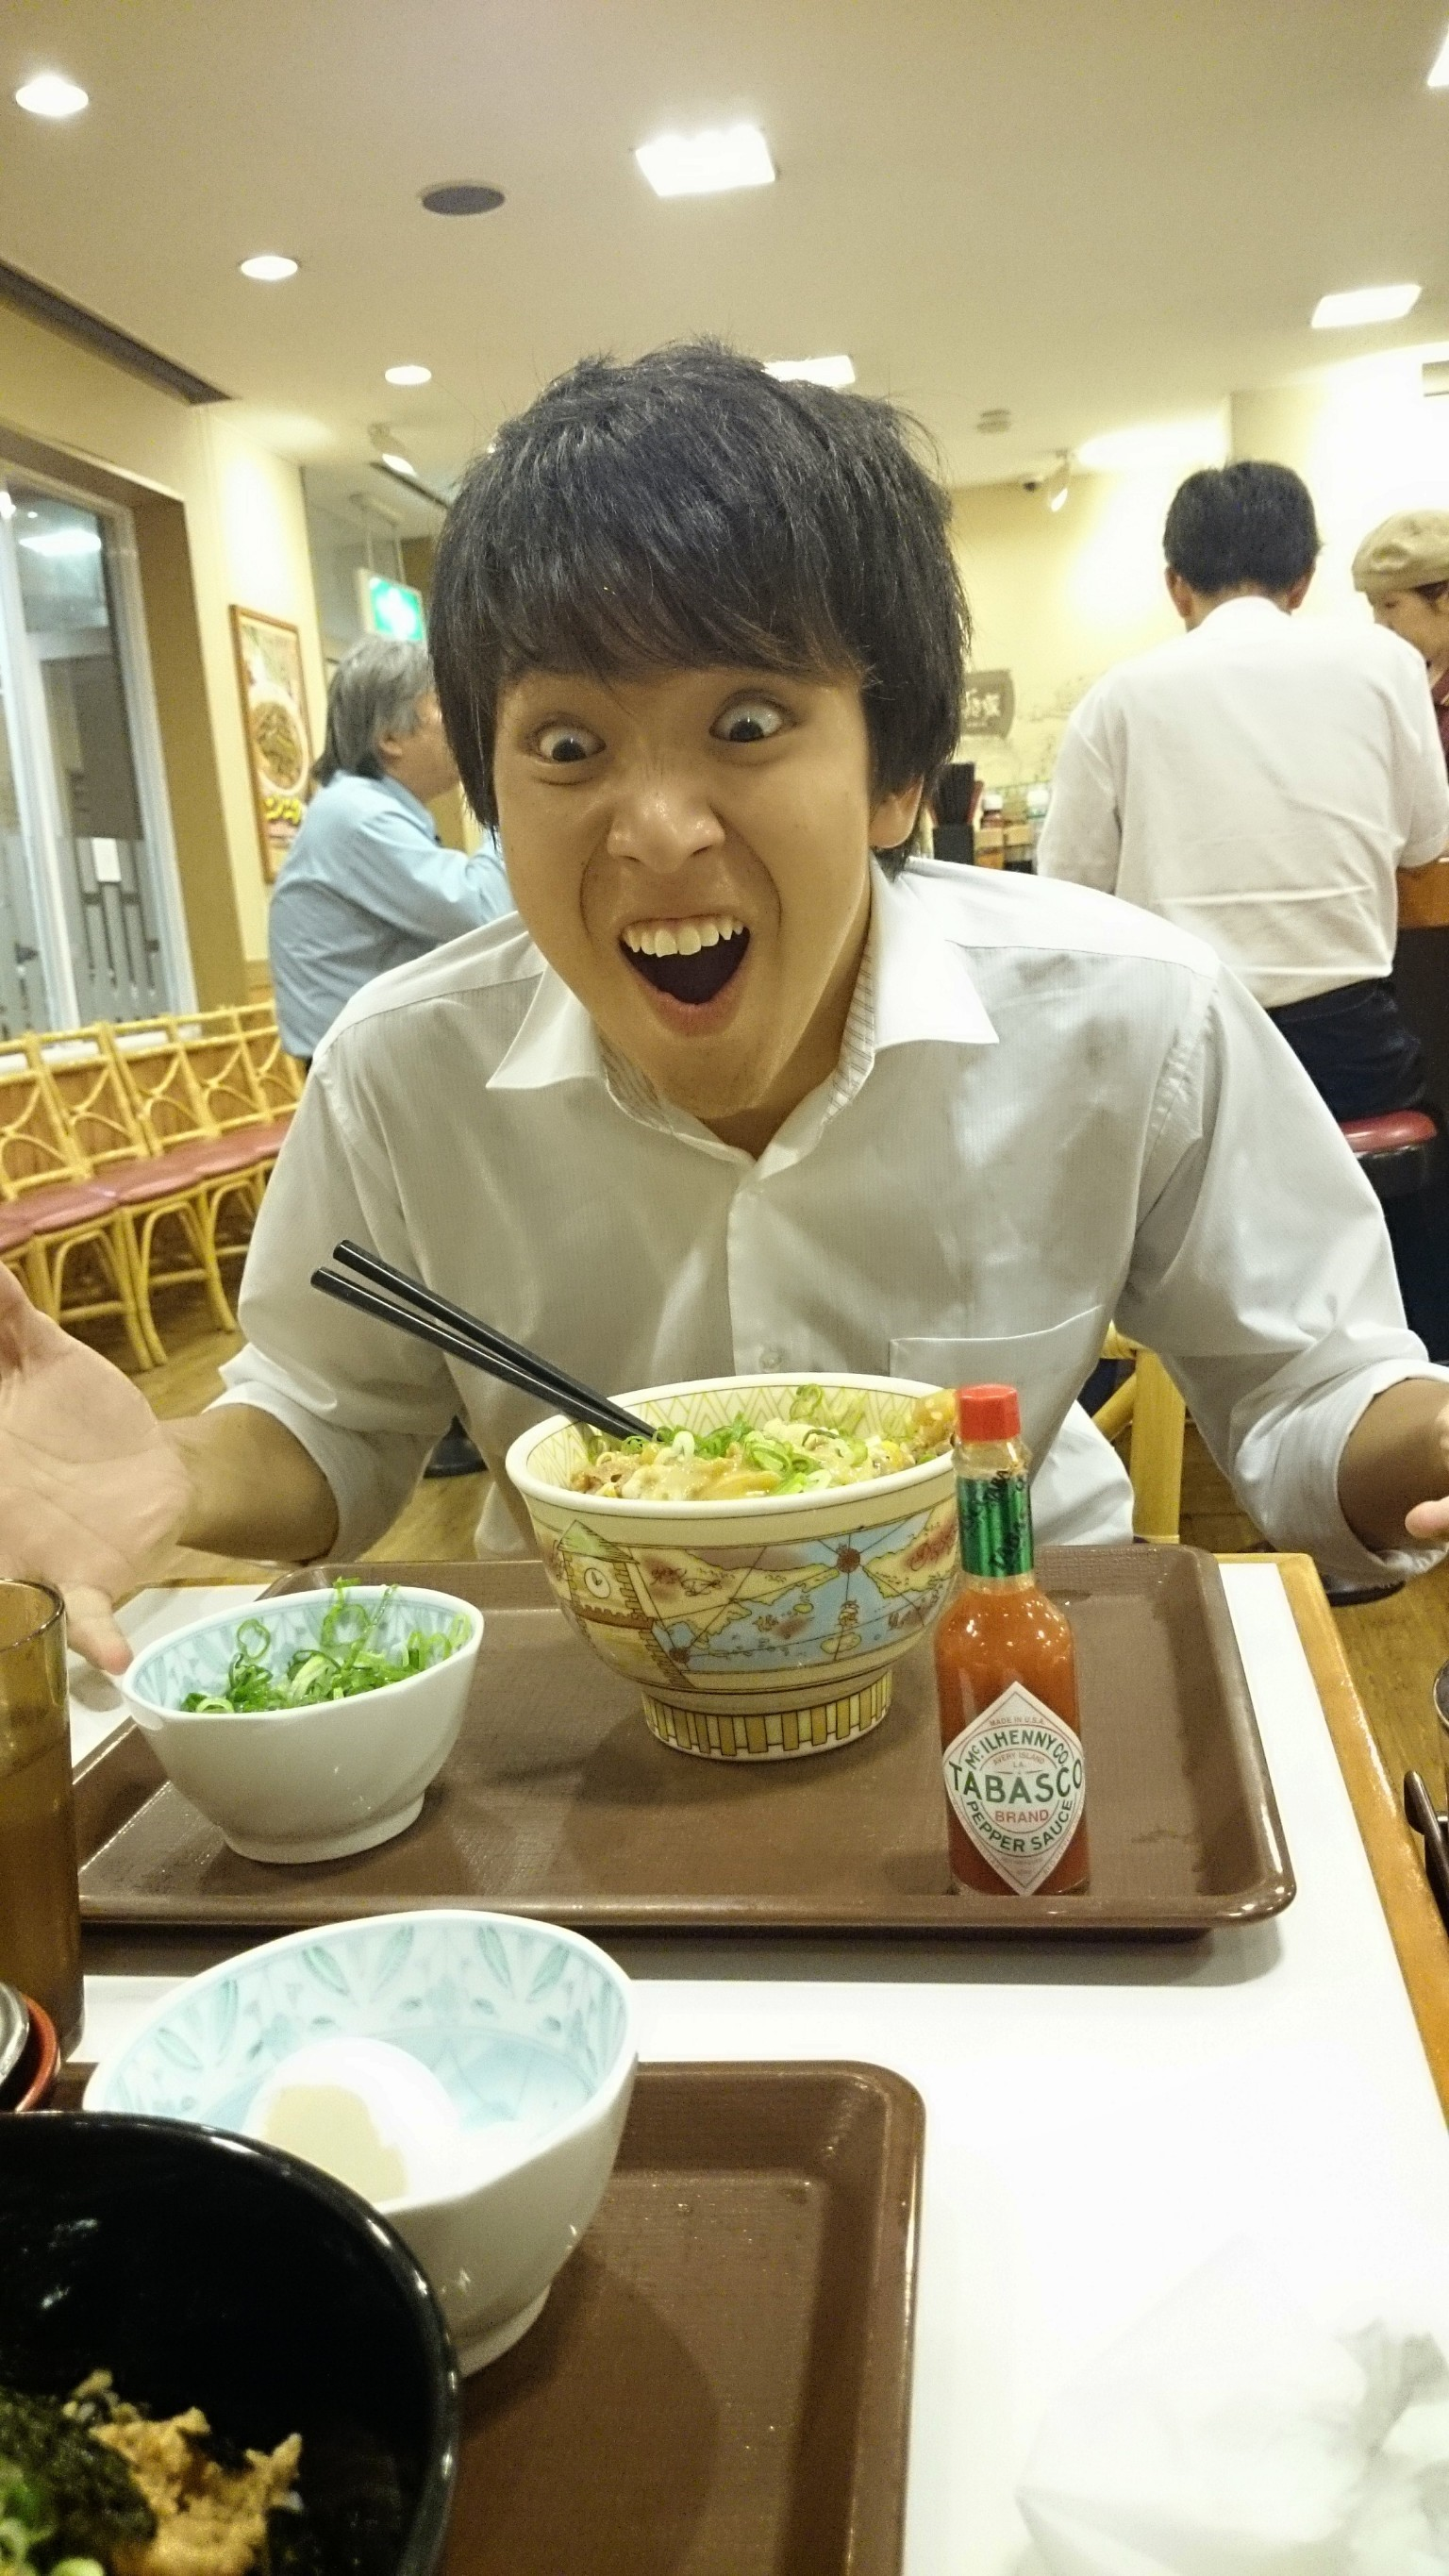
\includegraphics[width=0.3\textwidth]{./section/Shokuji/figures/LifeSukiya.jpg}
%  \end{center}
 \caption{とりあえず辛いもの食っとけの精神でタバスコを用意し、またネギ大盛り別皿はテッパンである。これをもりもり食べた後は、原動機付自転車を法定時速で運転し、家に帰って寝るだけである。}
  \label{fig:one}
\end{figure}
% \end{minipage}
% \begin{minipage}{0.5\hsize}
%  \begin{center}
\begin{figure}[htbp]
\centering
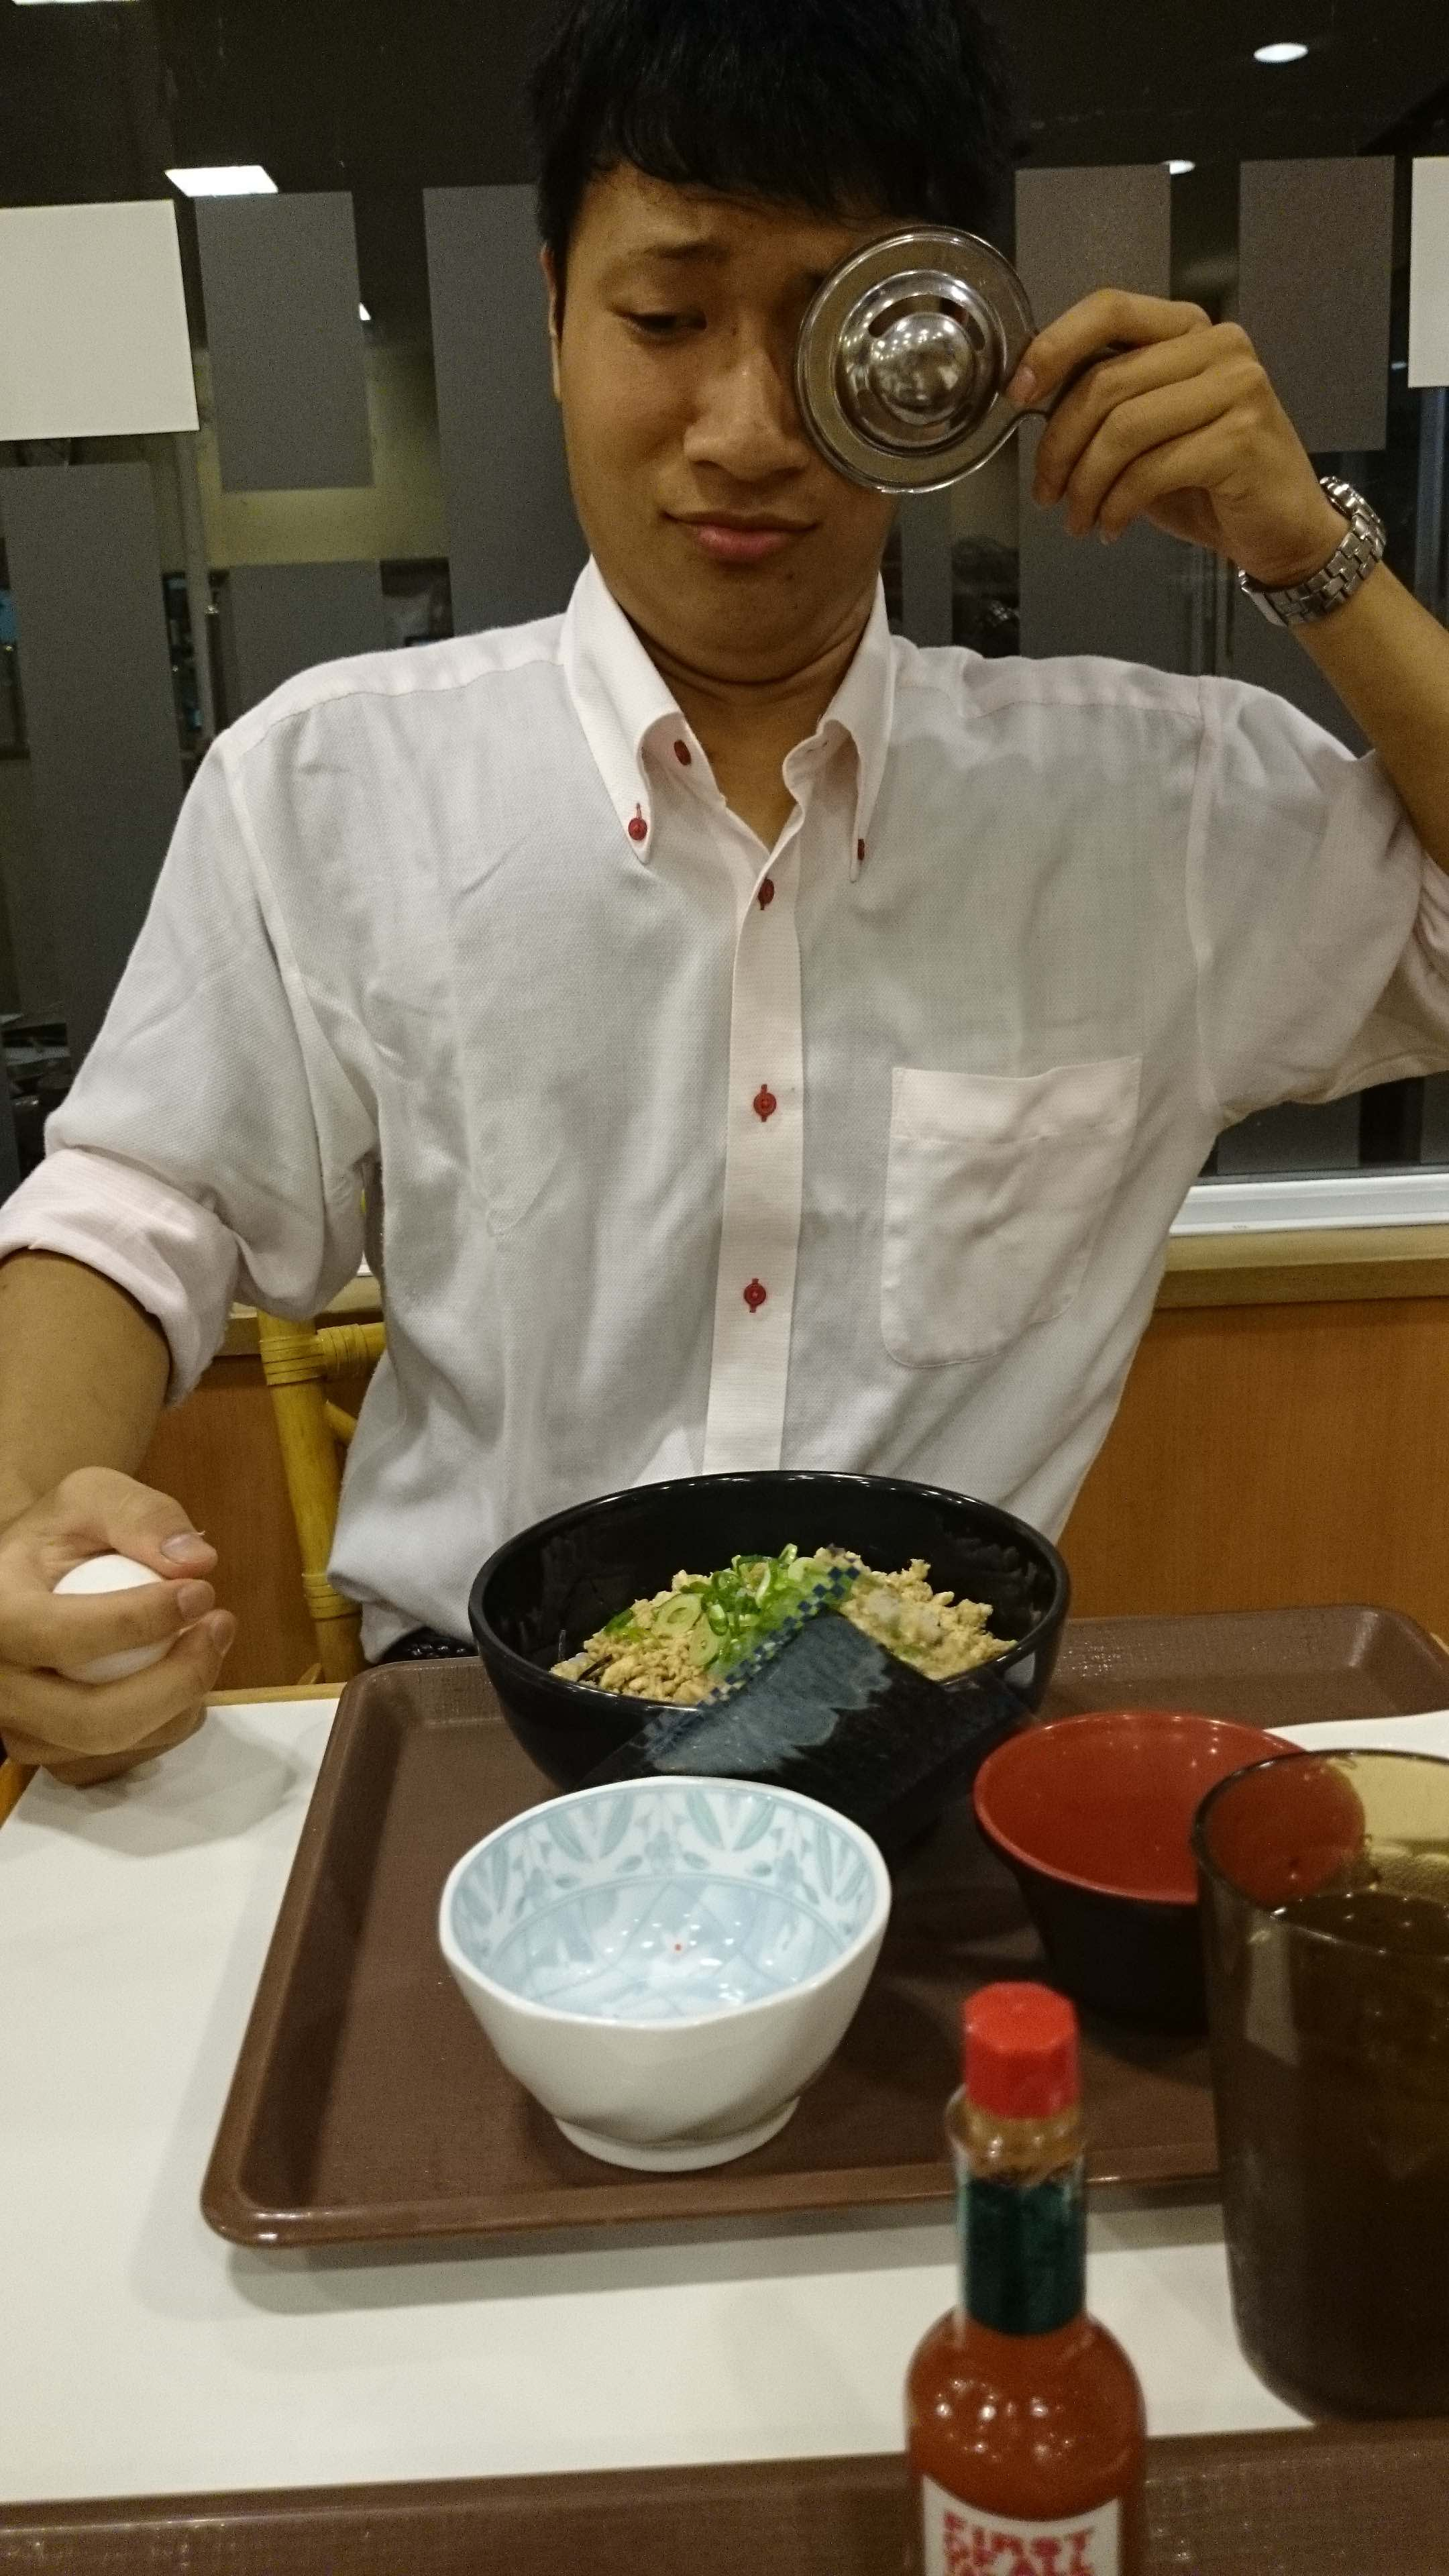
\includegraphics[width=0.3\textwidth]{./section/Shokuji/figures/LifeSukiya_2.jpg}
 \caption{この男はこの夜食を食った後、原動機付自転車を時速60km/hでぶっ飛ばし門限までに寮に帰らなければならないのである。さもなければ反省文を書かなければならない。法定時速を守るか、寮の規則を守るか。この男はあまりにも寮に忠実な(ちゃんと掃除会にも参加するし、なんか色々やるし)模範的な寮生なのであった。}
  \label{Fig:Ogawa}
\end{figure}

さらに、食べすぎたのか何なのか分からないが、別人とも言えるオガワの写真(図\ref{Fig:OgawaBetsujin})も現存している。
タケダ側のお盆を見ると、健康を気にしてサラダを頼んでいるが、焼け石に水、無駄な抵抗である。
それに引き換え、オガワは宙を見つめ、すべてを悟ったかのように己の運命を受け入れている。

% ----------------------------------------
\begin{figure}[h]
\centering
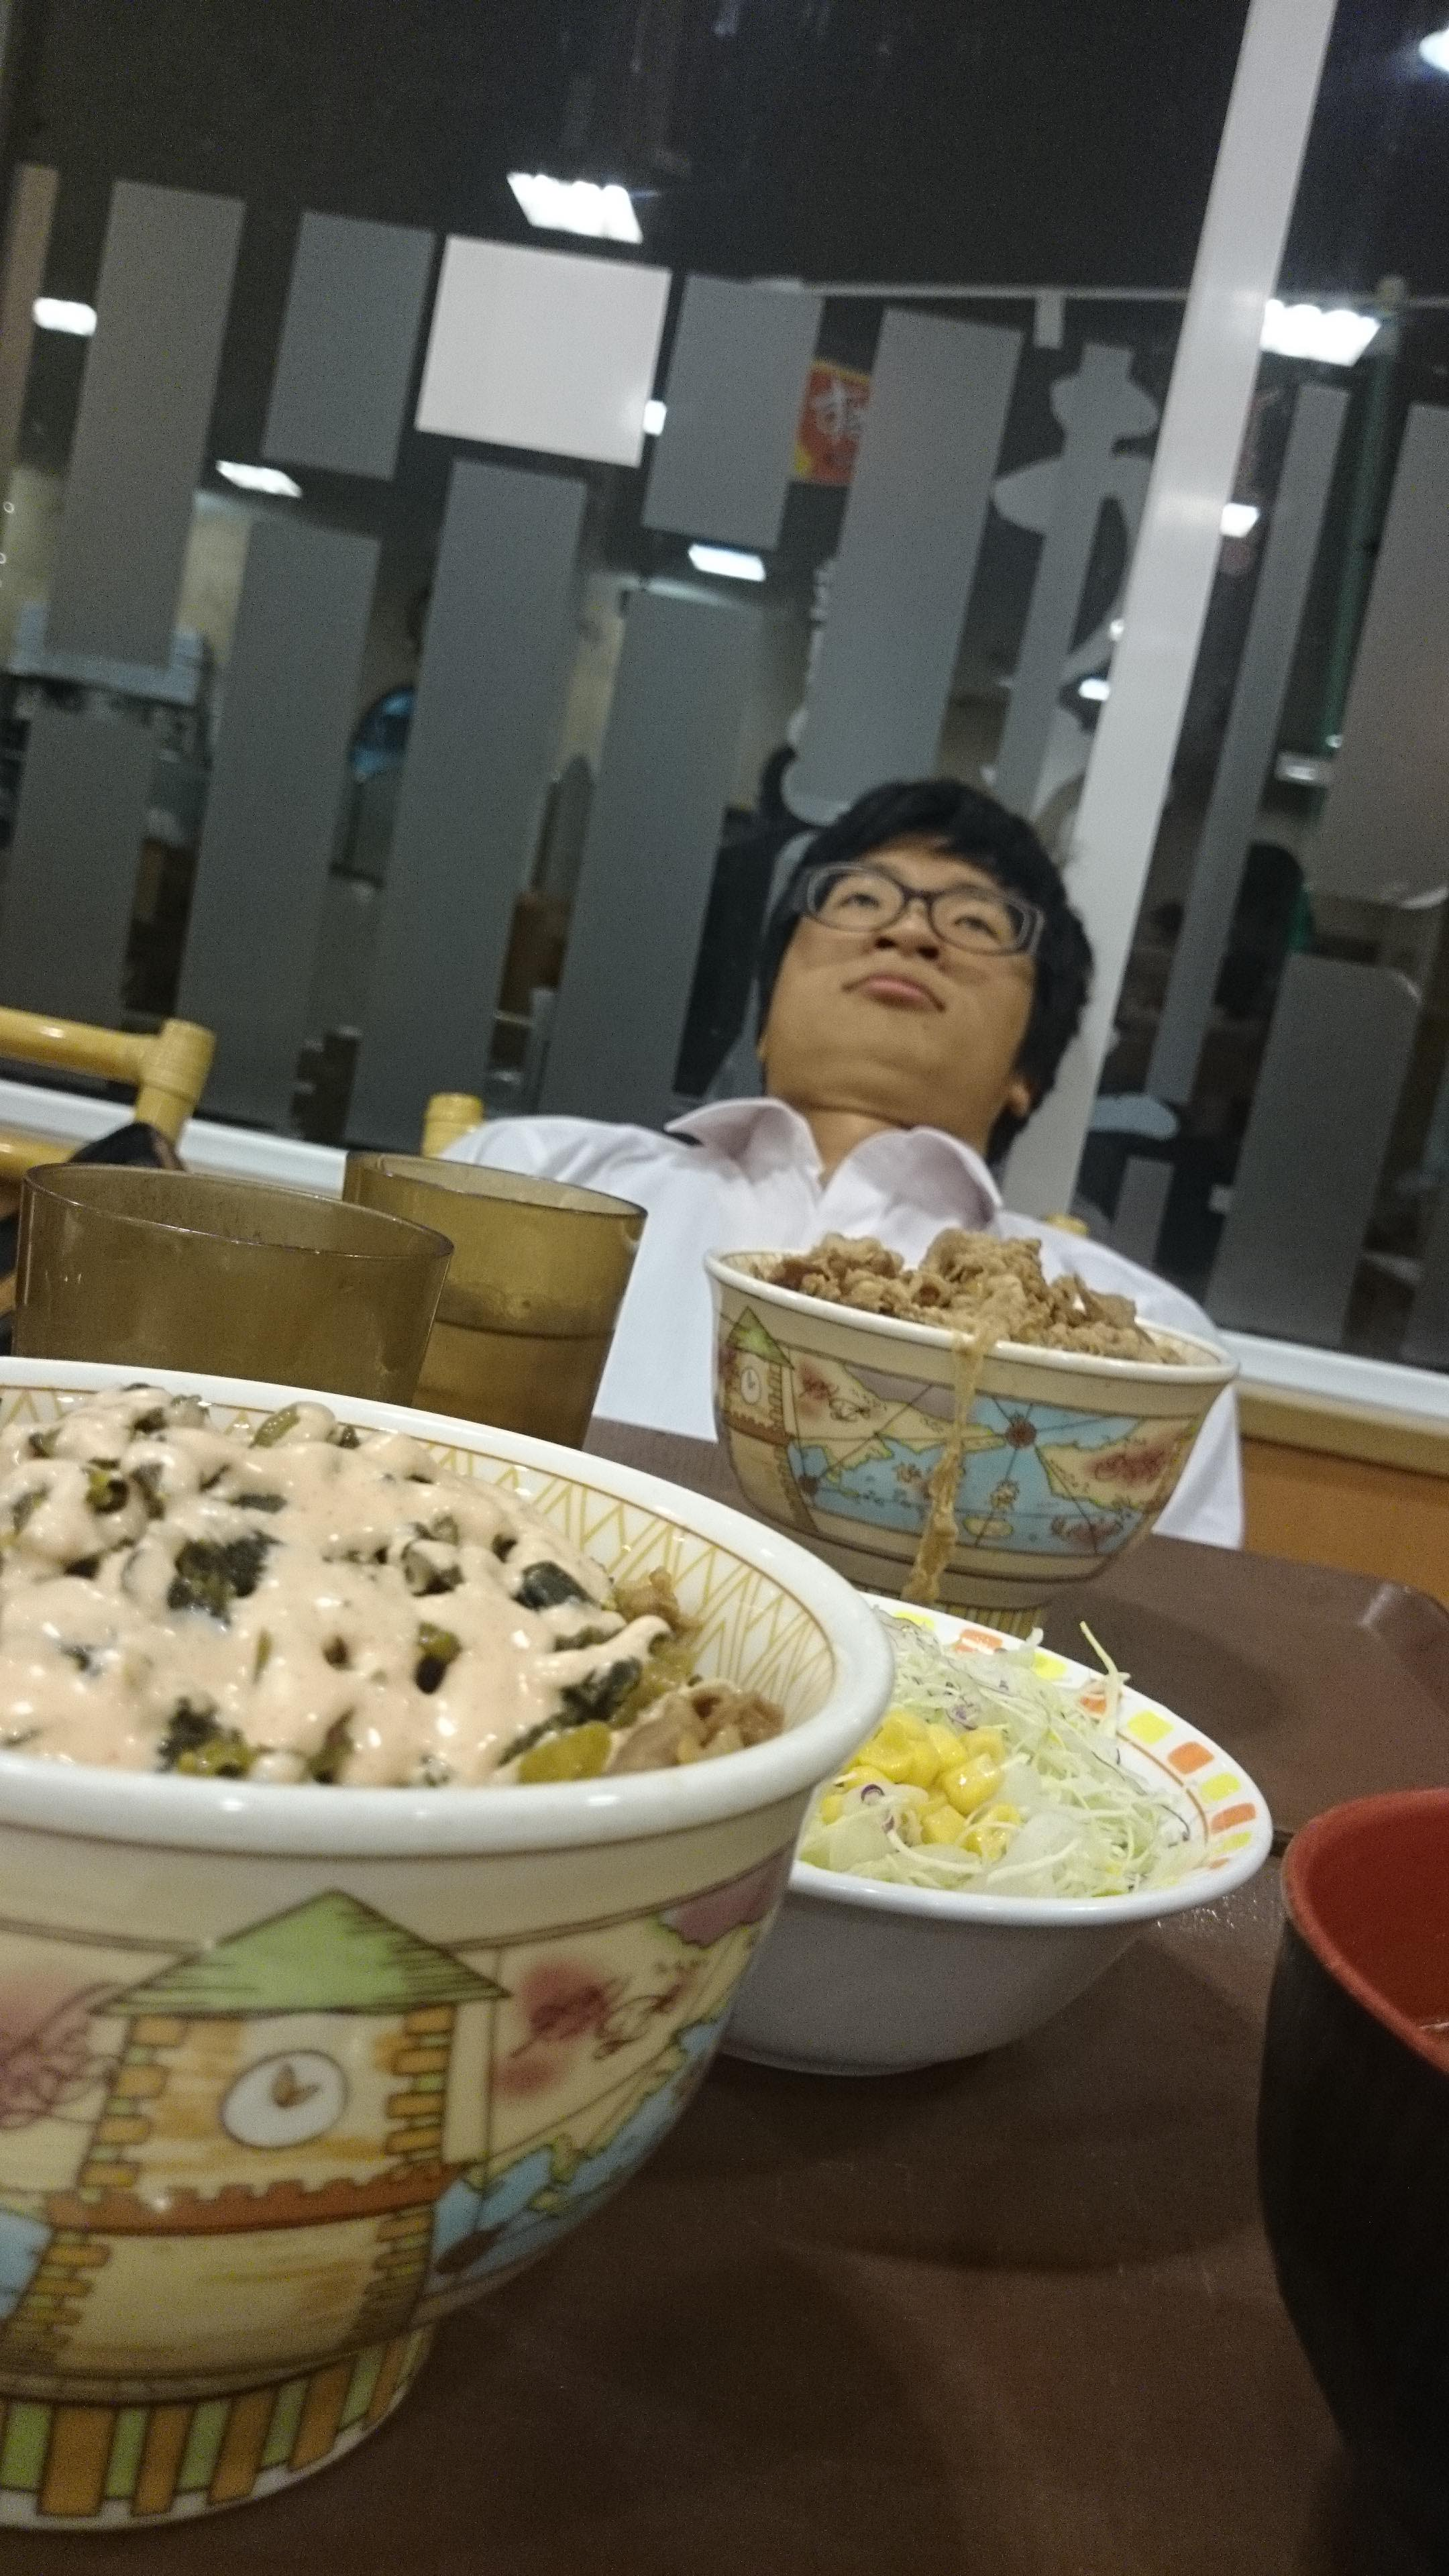
\includegraphics[width=0.3\textwidth]{./section/Shokuji/figures/LifeSukiya_3.jpg}
  \caption{図\ref{Fig:Ogawa}とはあまりにも別人の様に見える写真である。彼は今にも「バァァ」と言いたげな、物憂げな顔をしている。彼の頭の中は、時速60km/hのことで頭が一杯である(60km/hで走らないと、車線変更できず家に帰れないのである)。}
\label{Fig:OgawaBetsujin}
\end{figure}
% ----------------------------------------

%==========================%
\subsection{虎と龍}
%==========================%
また、彼らは(今は無き)虎と龍の替え玉祭りにも、バイト終わりに挑戦するという偉業を成し遂げている。
替え玉祭りとは、年に数回行われる、虎と龍の替え玉無料食べ放題キャンペーンであり、非常にお得なイベントである。
祭り素人は、バリカタであったりハリガネを頼むかもしれない。
しかし、そのような硬さを攻めていればスープは麺に持っていかれ、3玉目にはもはやスープがほぼない状態に陥ることもある。
かといって、ふつう、やわめを頼めば、1玉の体積は増えるので、これはこれで食べるのが非常に辛いのである。
そのような男の決断、英断を重ねて、ようやく5玉食いに到達できるのである。

% ----------------------------------------
\begin{figure}[h]
\centering
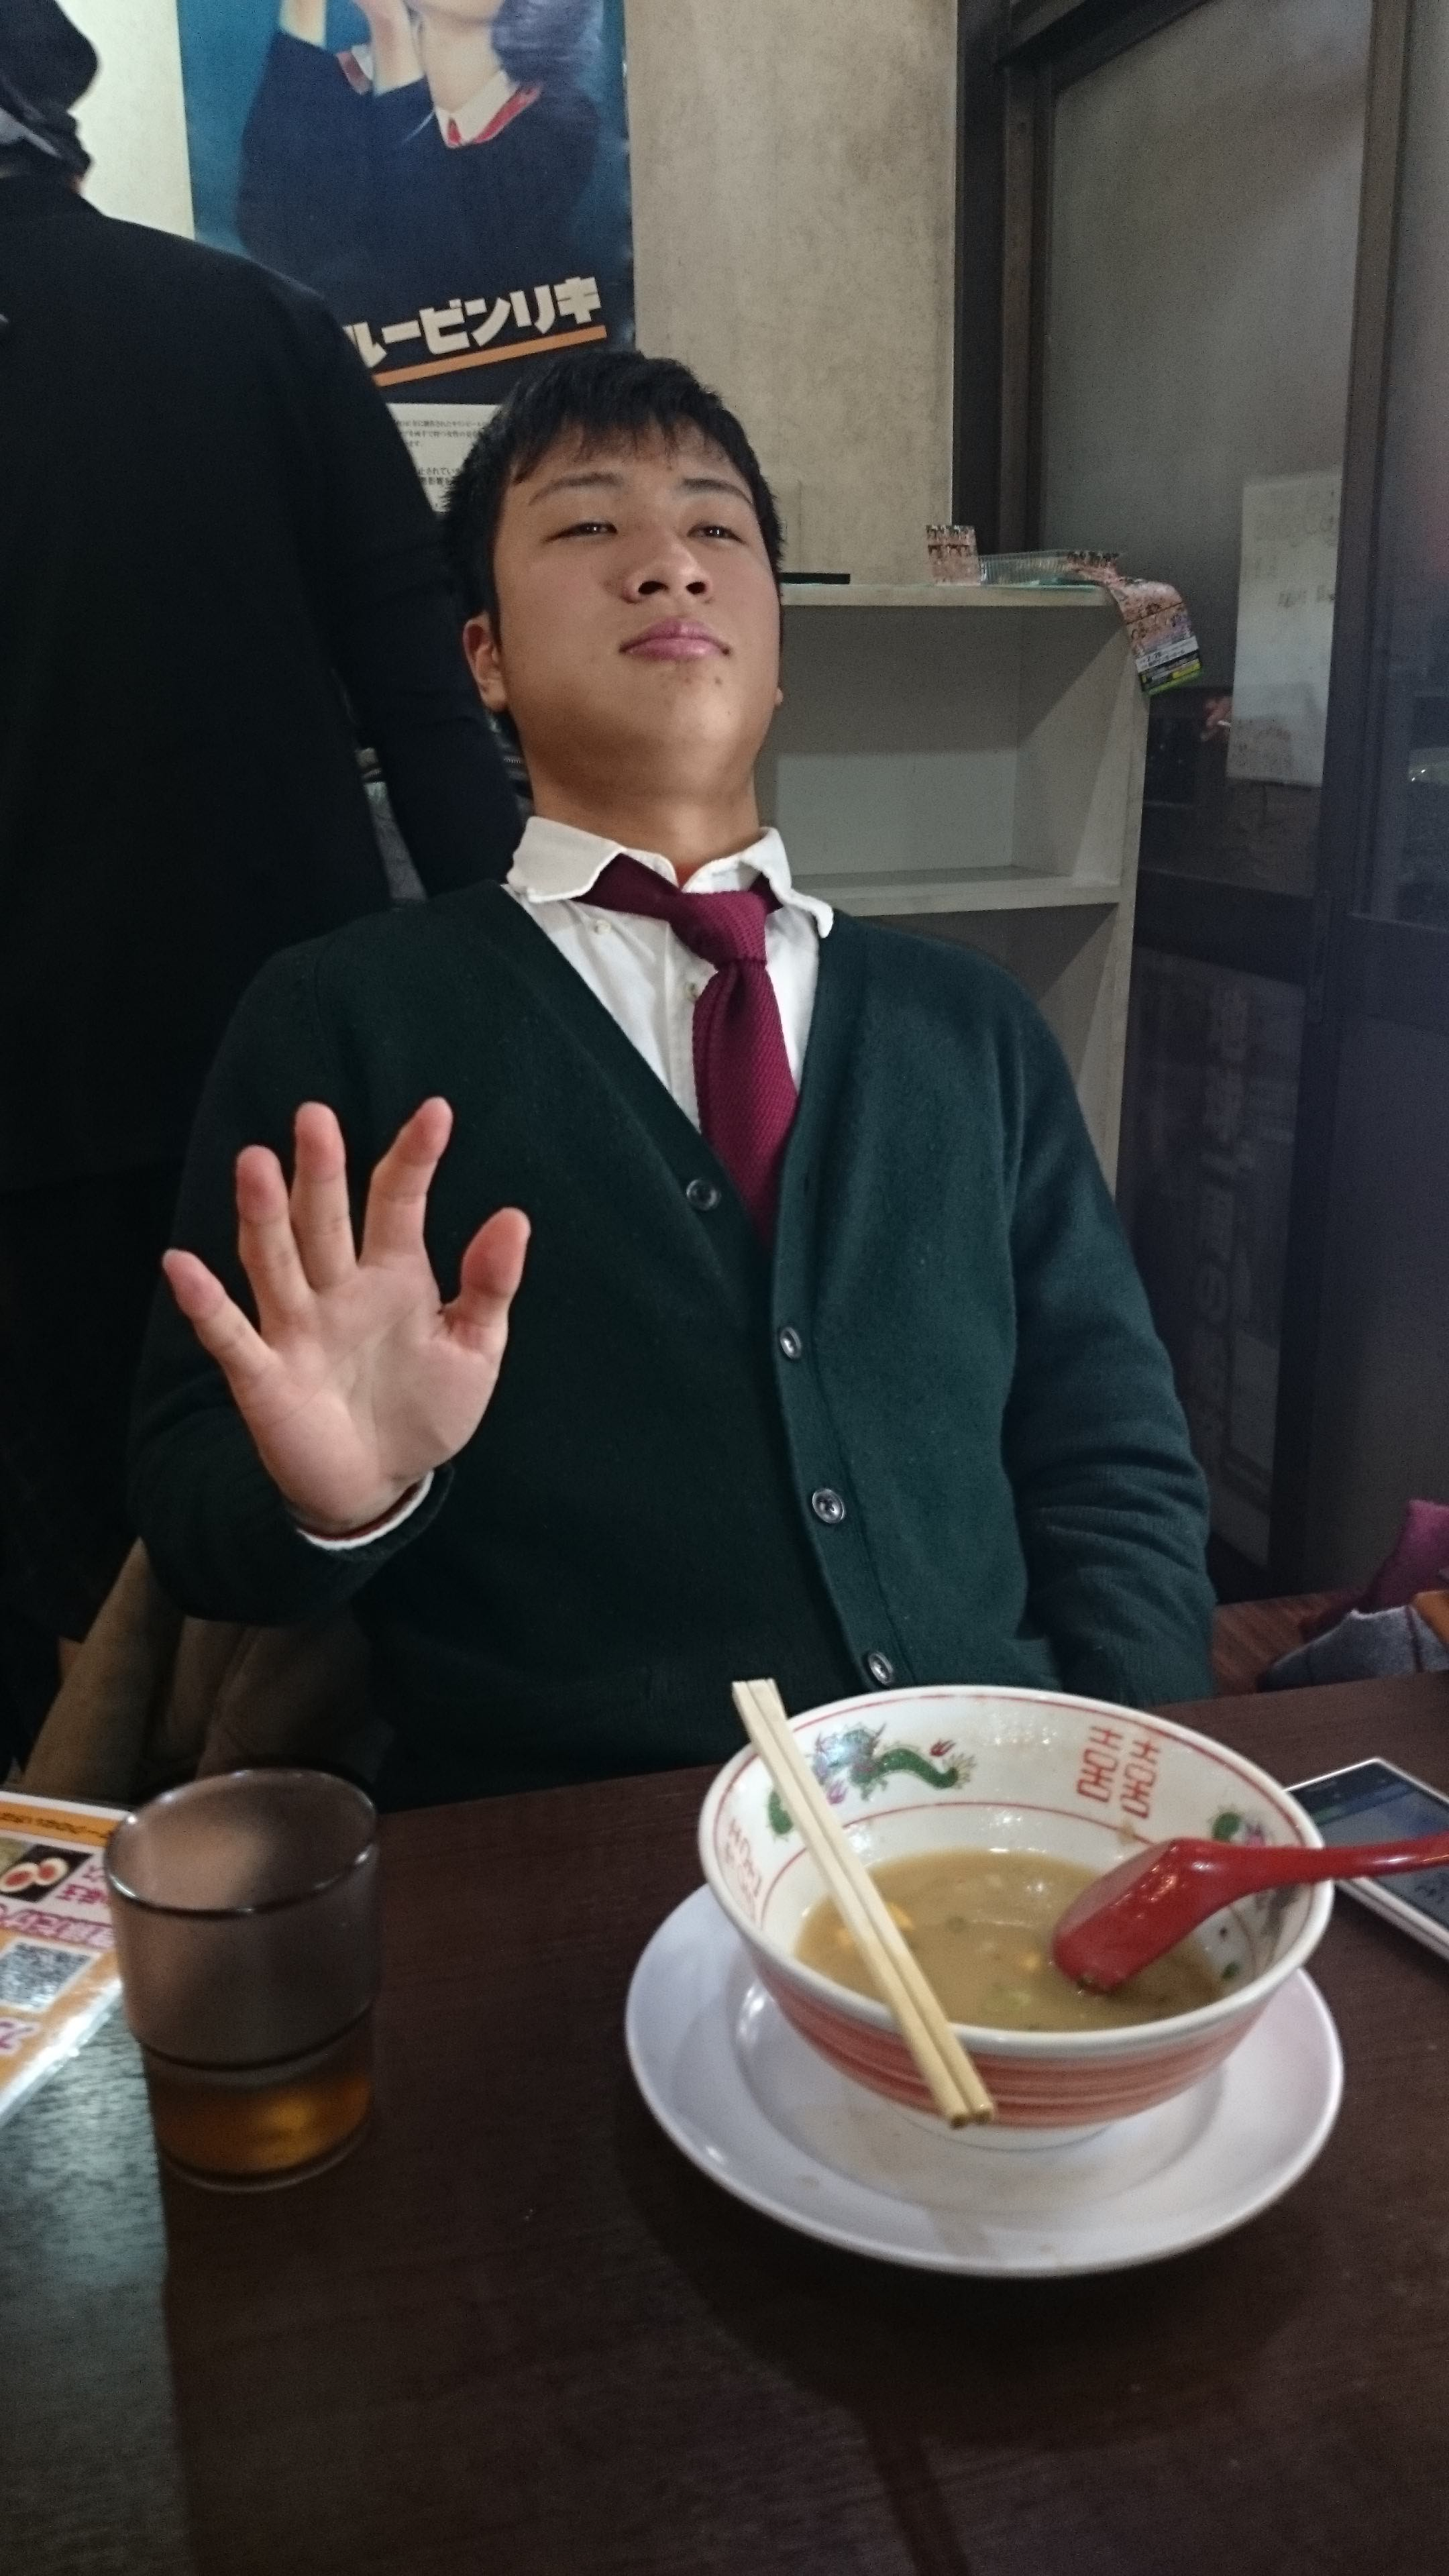
\includegraphics[width=0.3\textwidth]{./section/Shokuji/figures/Toraryuu_1.jpg}
  \caption{5玉をたいらげ、もはやギブアップ寸前のオガワ。ここから原動機付自転車を時速60km/hでぶっ飛ばし門限までに寮に帰らなければならないのである。このようにぶっ飛ばしまくり、またロクにオイル交換をしていなかったためか、晩年のオガワバイクは最高時速が40km/hに落ちることとなる。原付、晩年はエンジンかかりにくかったんやけど、晩年にマタヨととびえもん太郎とくら寿司にいく約束してて、俺だけ原付で満を持して出発しようとしたら急死して徒歩遅刻したという。そして後に、なんとか動かしつつ近所のバイク屋に持ってって、重症患者の認定を受け、廃車宣言をし、交渉の末、無料でその日に廃車が決定した。}
\label{Fig:Seiza}
\end{figure}
% ----------------------------------------

%==========================%
\subsection{ちなみに}
%==========================%
ライフオガワ店は、晩年まで「実習中」であることが知られており、
いかにライフにおける作業を体得するのに時間がかかるかが分かるであろう。

% ----------------------------------------
\begin{figure}[h]
\centering
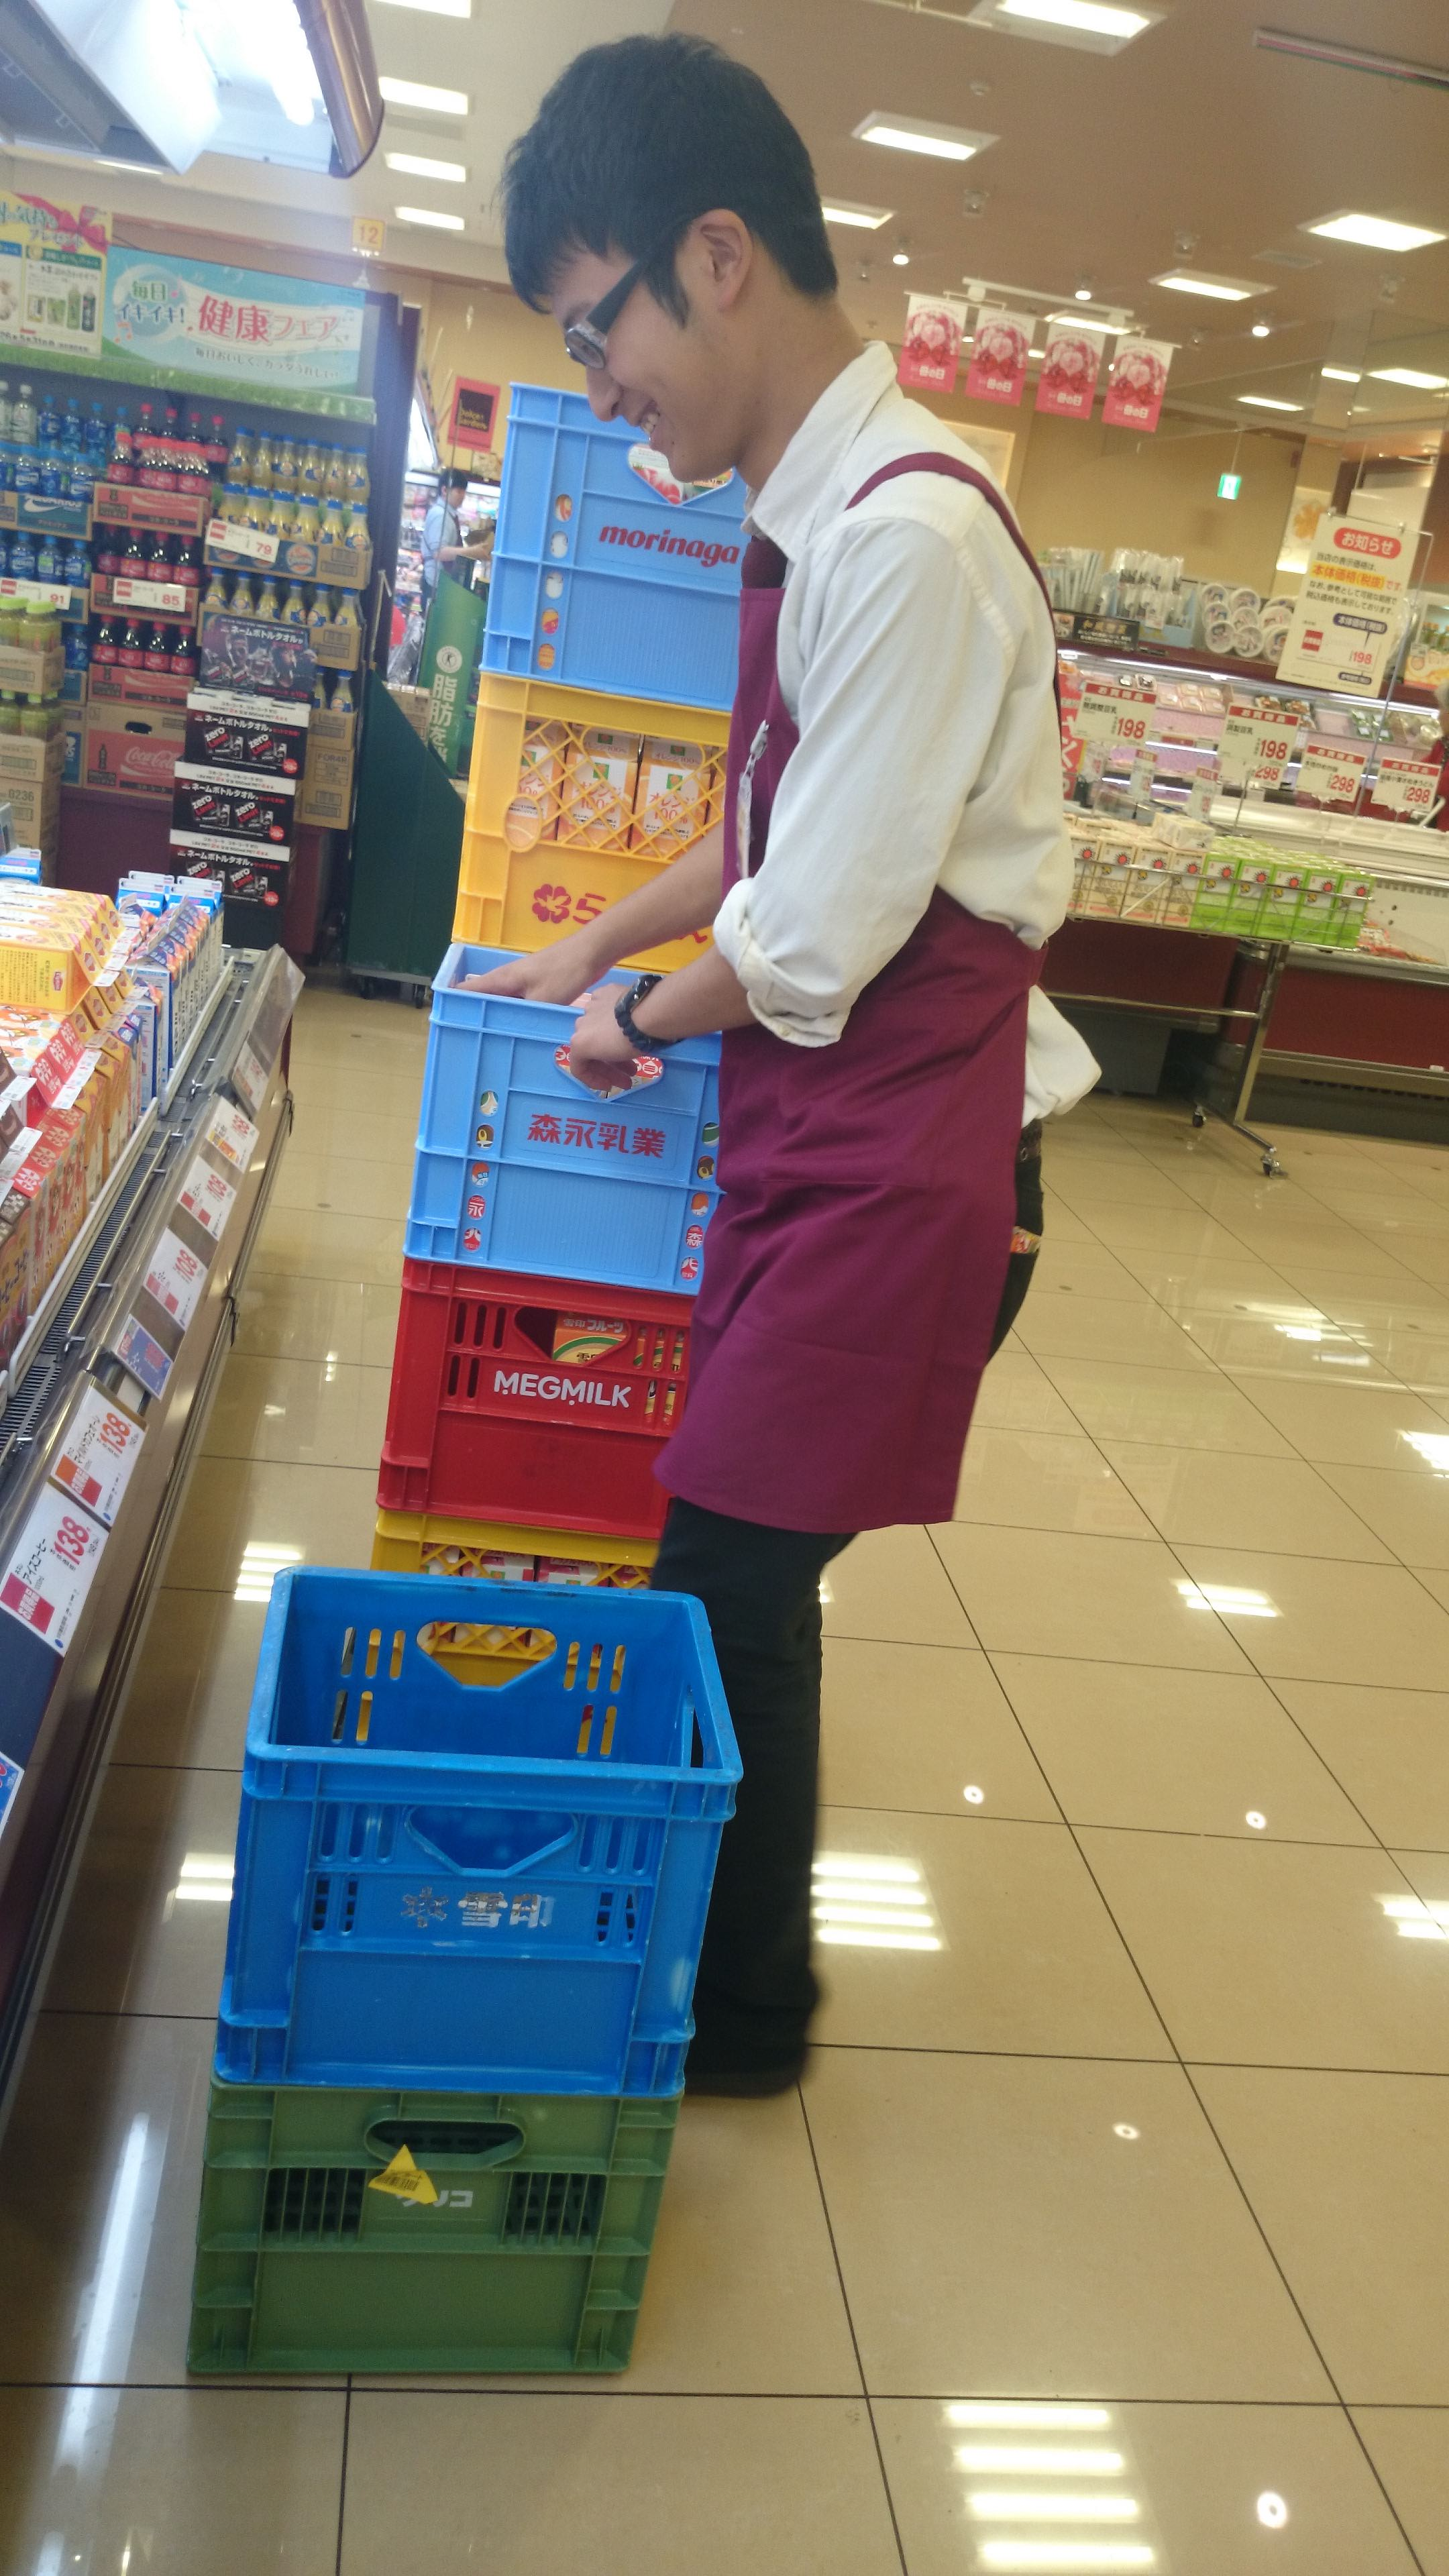
\includegraphics[width=0.3\textwidth]{./section/Shokuji/figures/Life_byte.jpg}
  \caption{バイト中の奇跡の一枚。彼は常に仕事をしつつ、パクれるものがないか品定めをしているのである。自らが欲する商品を見つけた場合、図の様に不敵な笑みを浮かべ、}
\label{Fig:Seiza}
\end{figure}
% ----------------------------------------

%%%%%%%%%%%%%%%%%%%%%%%%%%%%%%%%%%
\section{初めての阪神甲子園球場}
%%%%%%%%%%%%%%%%%%%%%%%%%%%%%%%%%%
ライフでの勤務により、超越した晩御飯を経験する回数が非常に増えたわけであるが、
食事だけでなく睡眠時間さえも通常の睡眠を超越した日があった。
それが、甲子園球場殴り込みの日である。
彼らはライフでの勤務が終わると(ごくたまにレジを悪用し、半額祭りを行っていたのだが)、双眼鏡を購入するためにドン・キホーテへと駆け込んだ。
そして一旦家へ帰り、仮眠を取る。
翌朝3時に起床し、始発で甲子園駅に行くためである。

\subsection{阪神甲子園球場}
甲子園駅に付いたものの、降車する人の先頭をきって動くことになってしまったため、全くどちらへ行ってよいか分からない彼らにとって、特に方向に感度を持たない特定の人物にとって、非常に困惑した事態となった。
標識もロクにでていないため、なんとなくで向かっていき正しいことが分かると、やがて、早足になり最後には駆け足で、入場の列へと殴り込むことになる。

% ----------------------------------------
\begin{figure}[h]
\centering
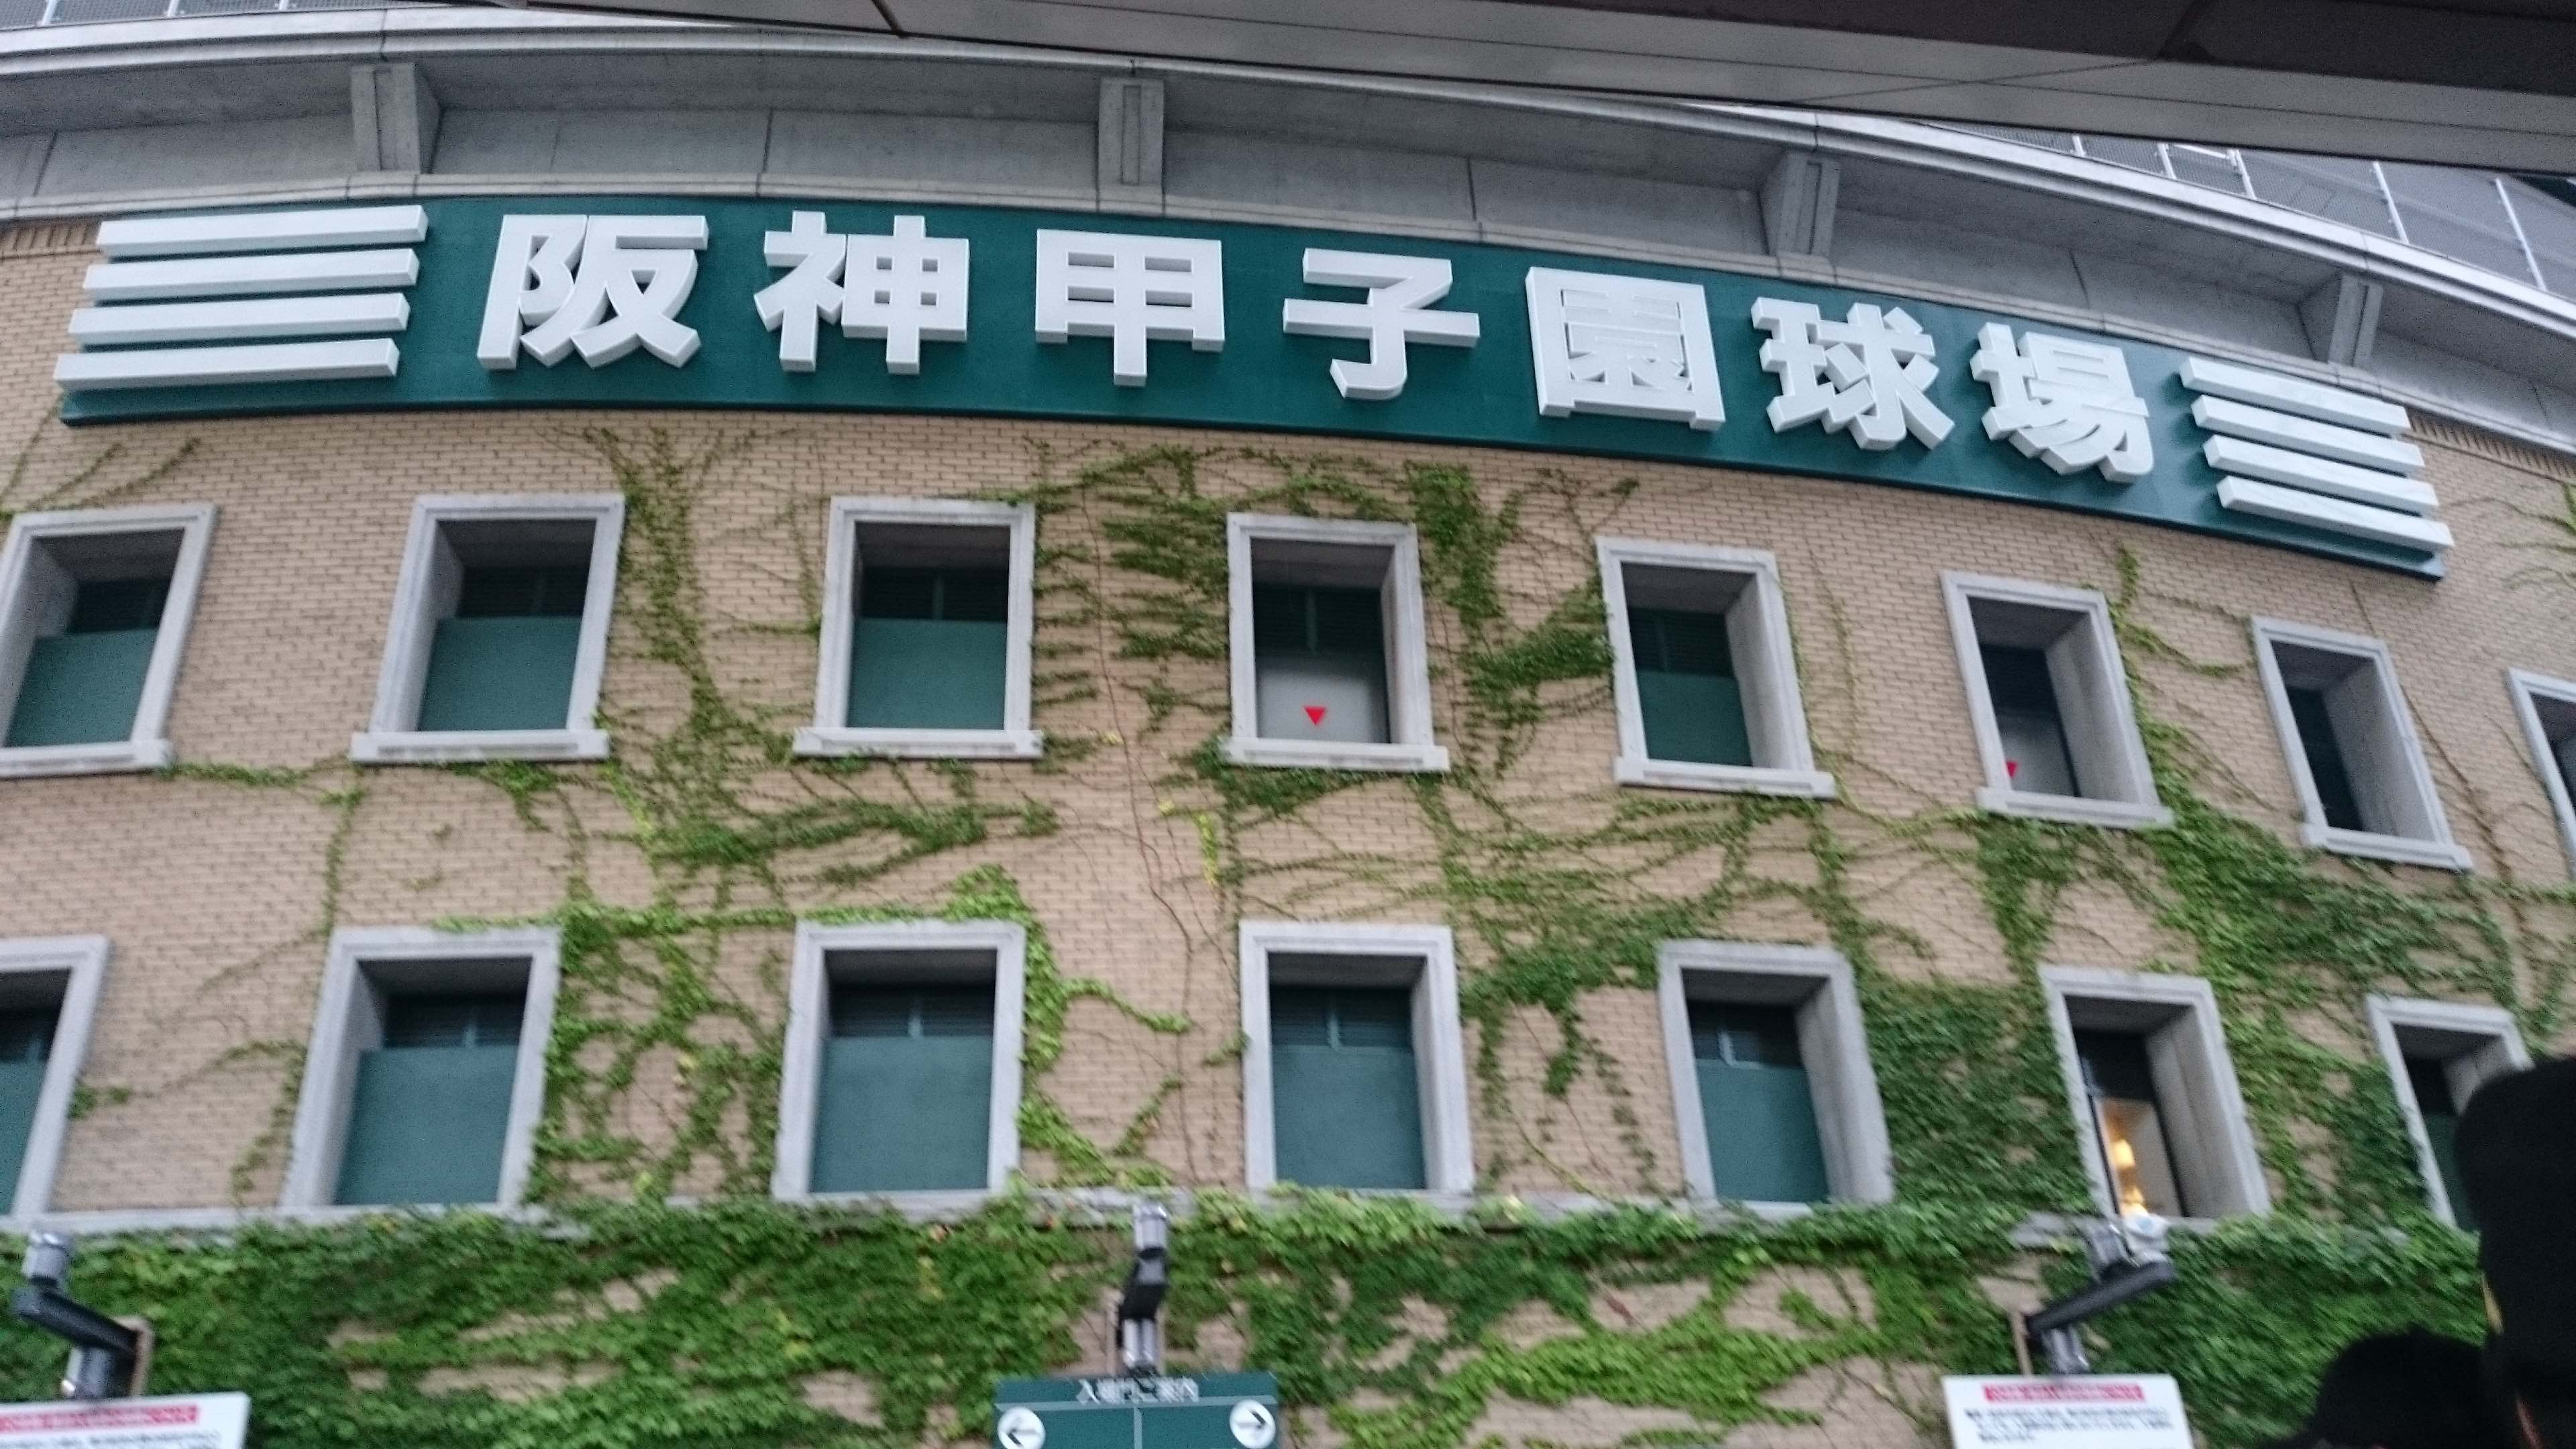
\includegraphics[width=0.7\textwidth]{./section/Shokuji/figures/Koushien_1.jpg}
  \caption{ついに見えた阪神甲子園球場。これから殴り込みに行くのである。}
\label{Fig:Seiza}
\end{figure}
% ----------------------------------------



\subsection{朝食という概念}
早朝3時に起きたため、もちろん到着した段階でお腹が空いており、近くのマクドナルドで朝マック持ち帰りを行うこととした。


% ----------------------------------------
\begin{figure}[h]
\centering
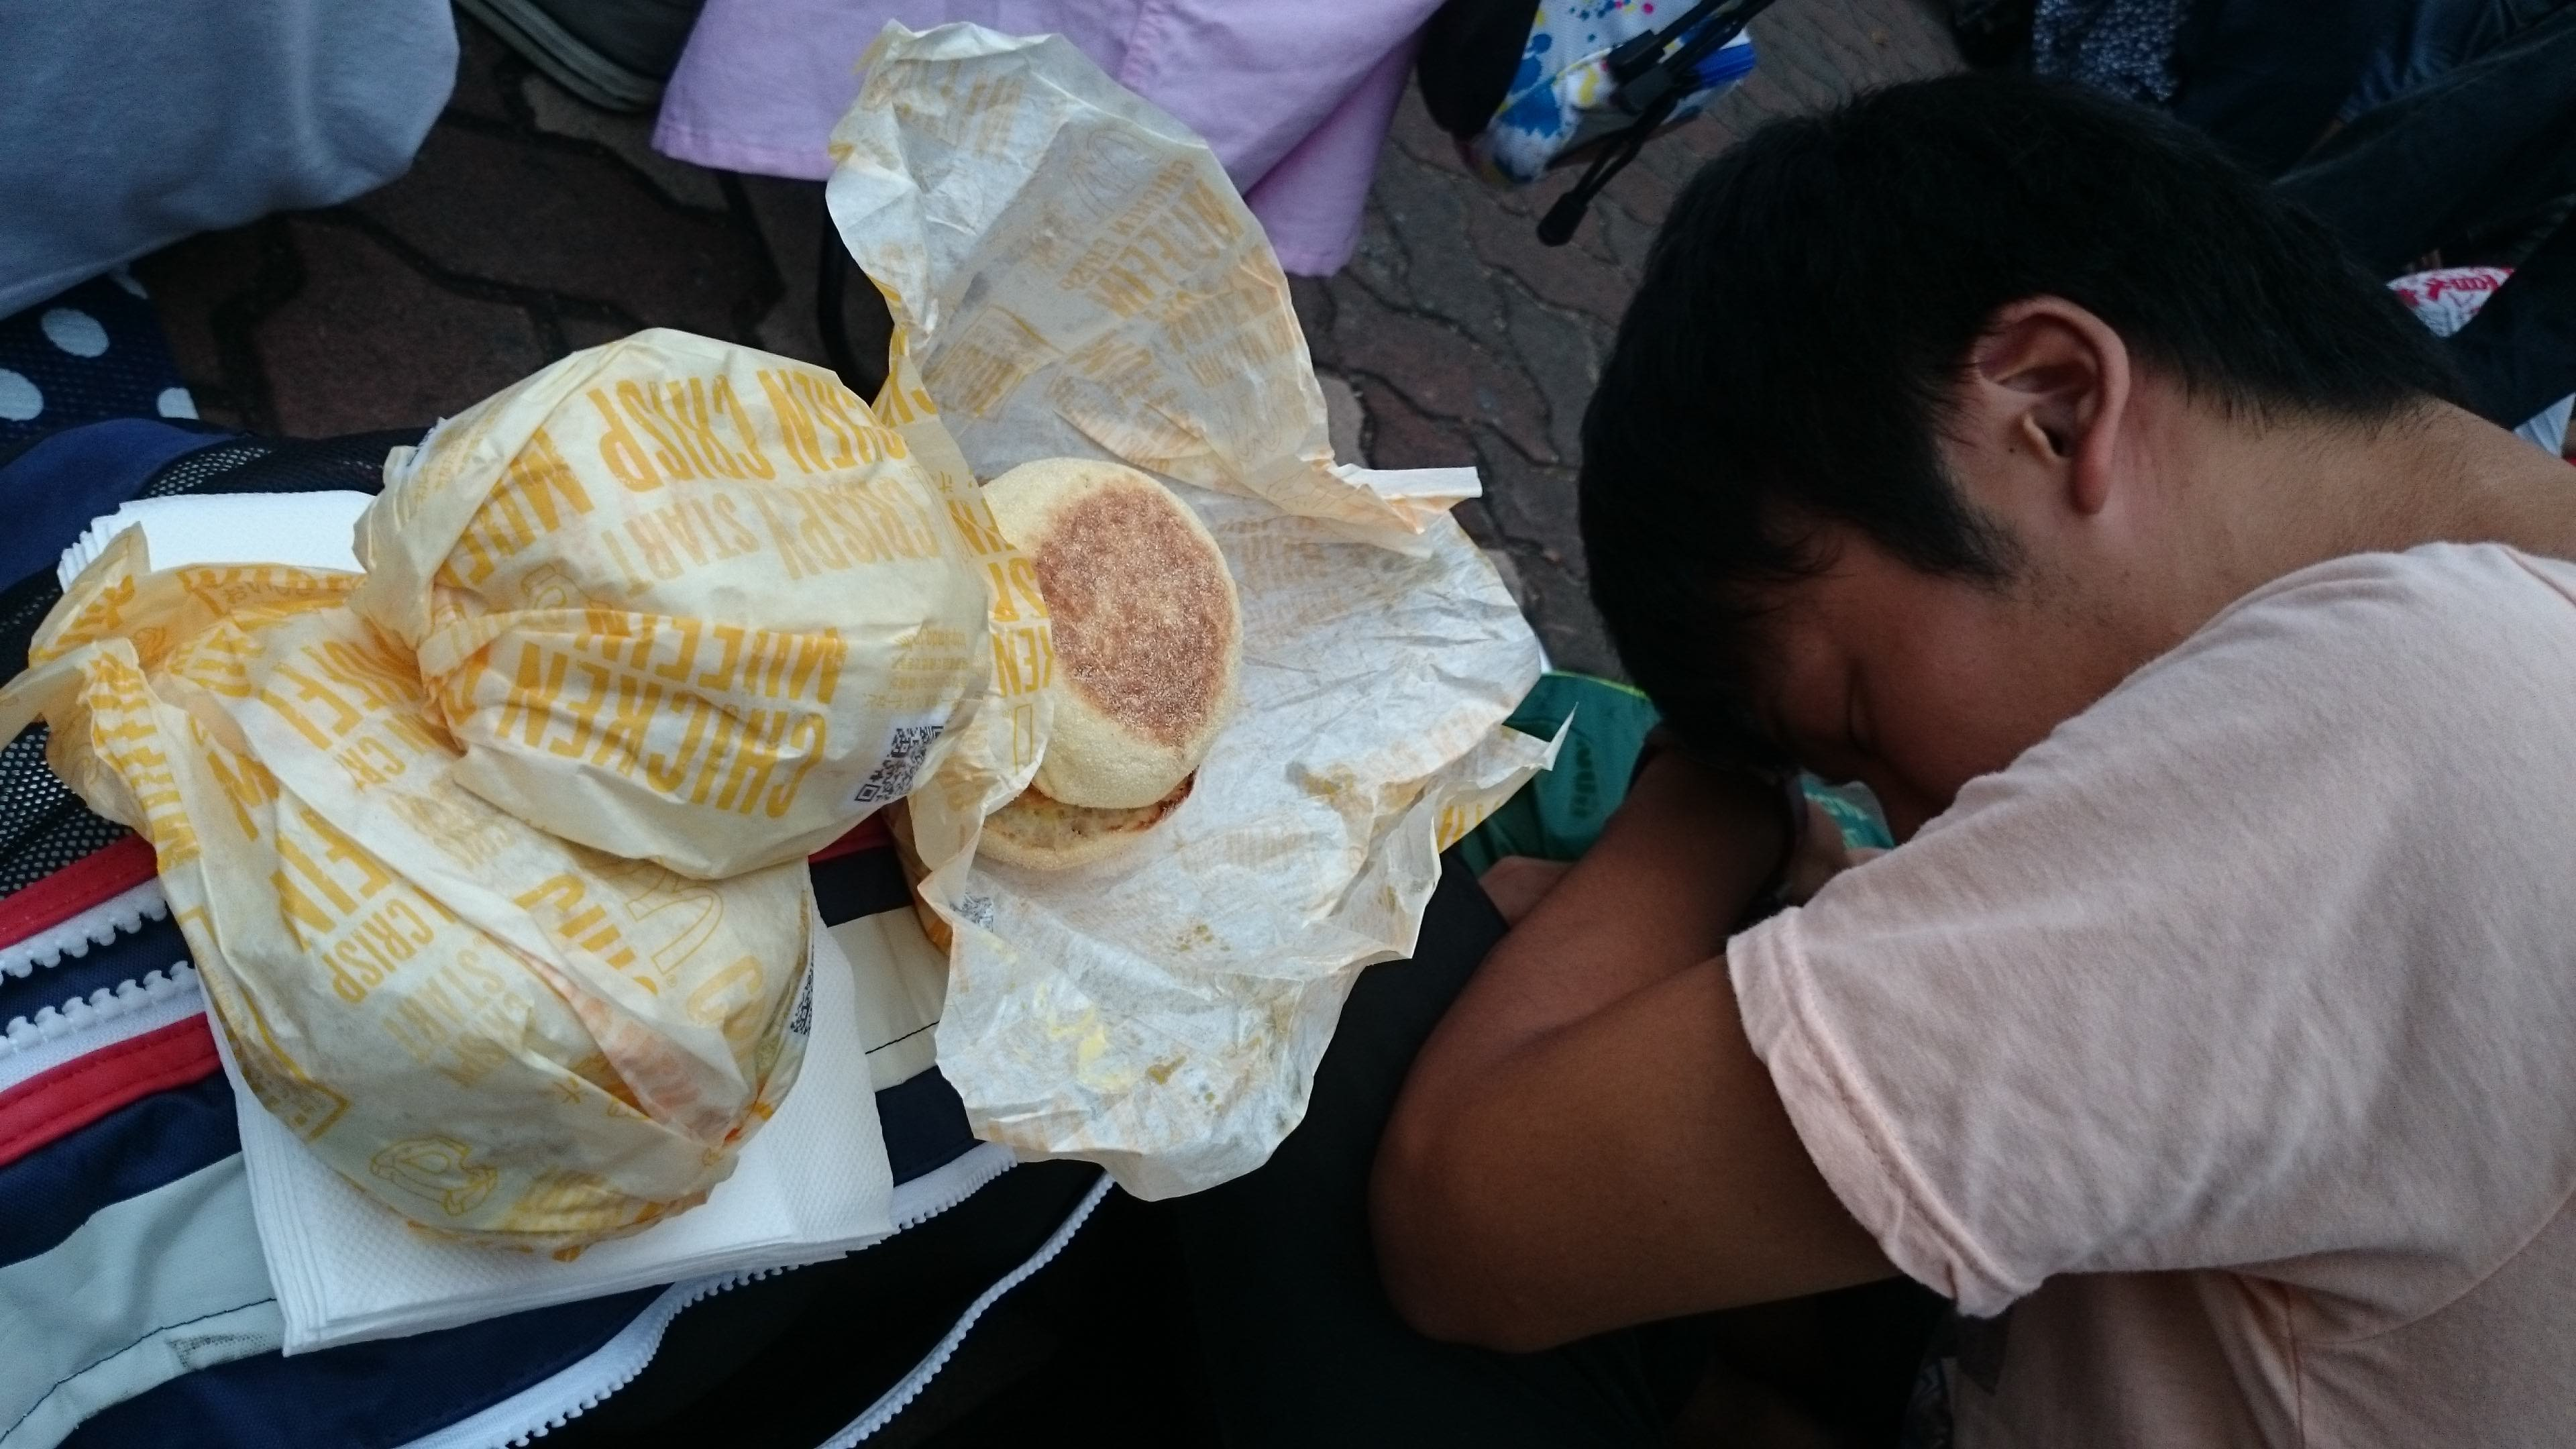
\includegraphics[width=0.7\textwidth]{./section/Shokuji/figures/Koushien_breakfast.jpg}
  \caption{持ち帰ってきた朝マックたち。彼は既に死んでいる。}
\label{Fig:Seiza}
\end{figure}
% ----------------------------------------


\subsection{殴り込みに当日の対戦カード}
野球をよく分からない人間でも知っている高校が出場しているので、たぶん良い日なのだろう。
たしか、この日の夕方にも何故かバイトを入れていたので、途中で早退したのであるが。

% ----------------------------------------
\begin{figure}[h]
\centering
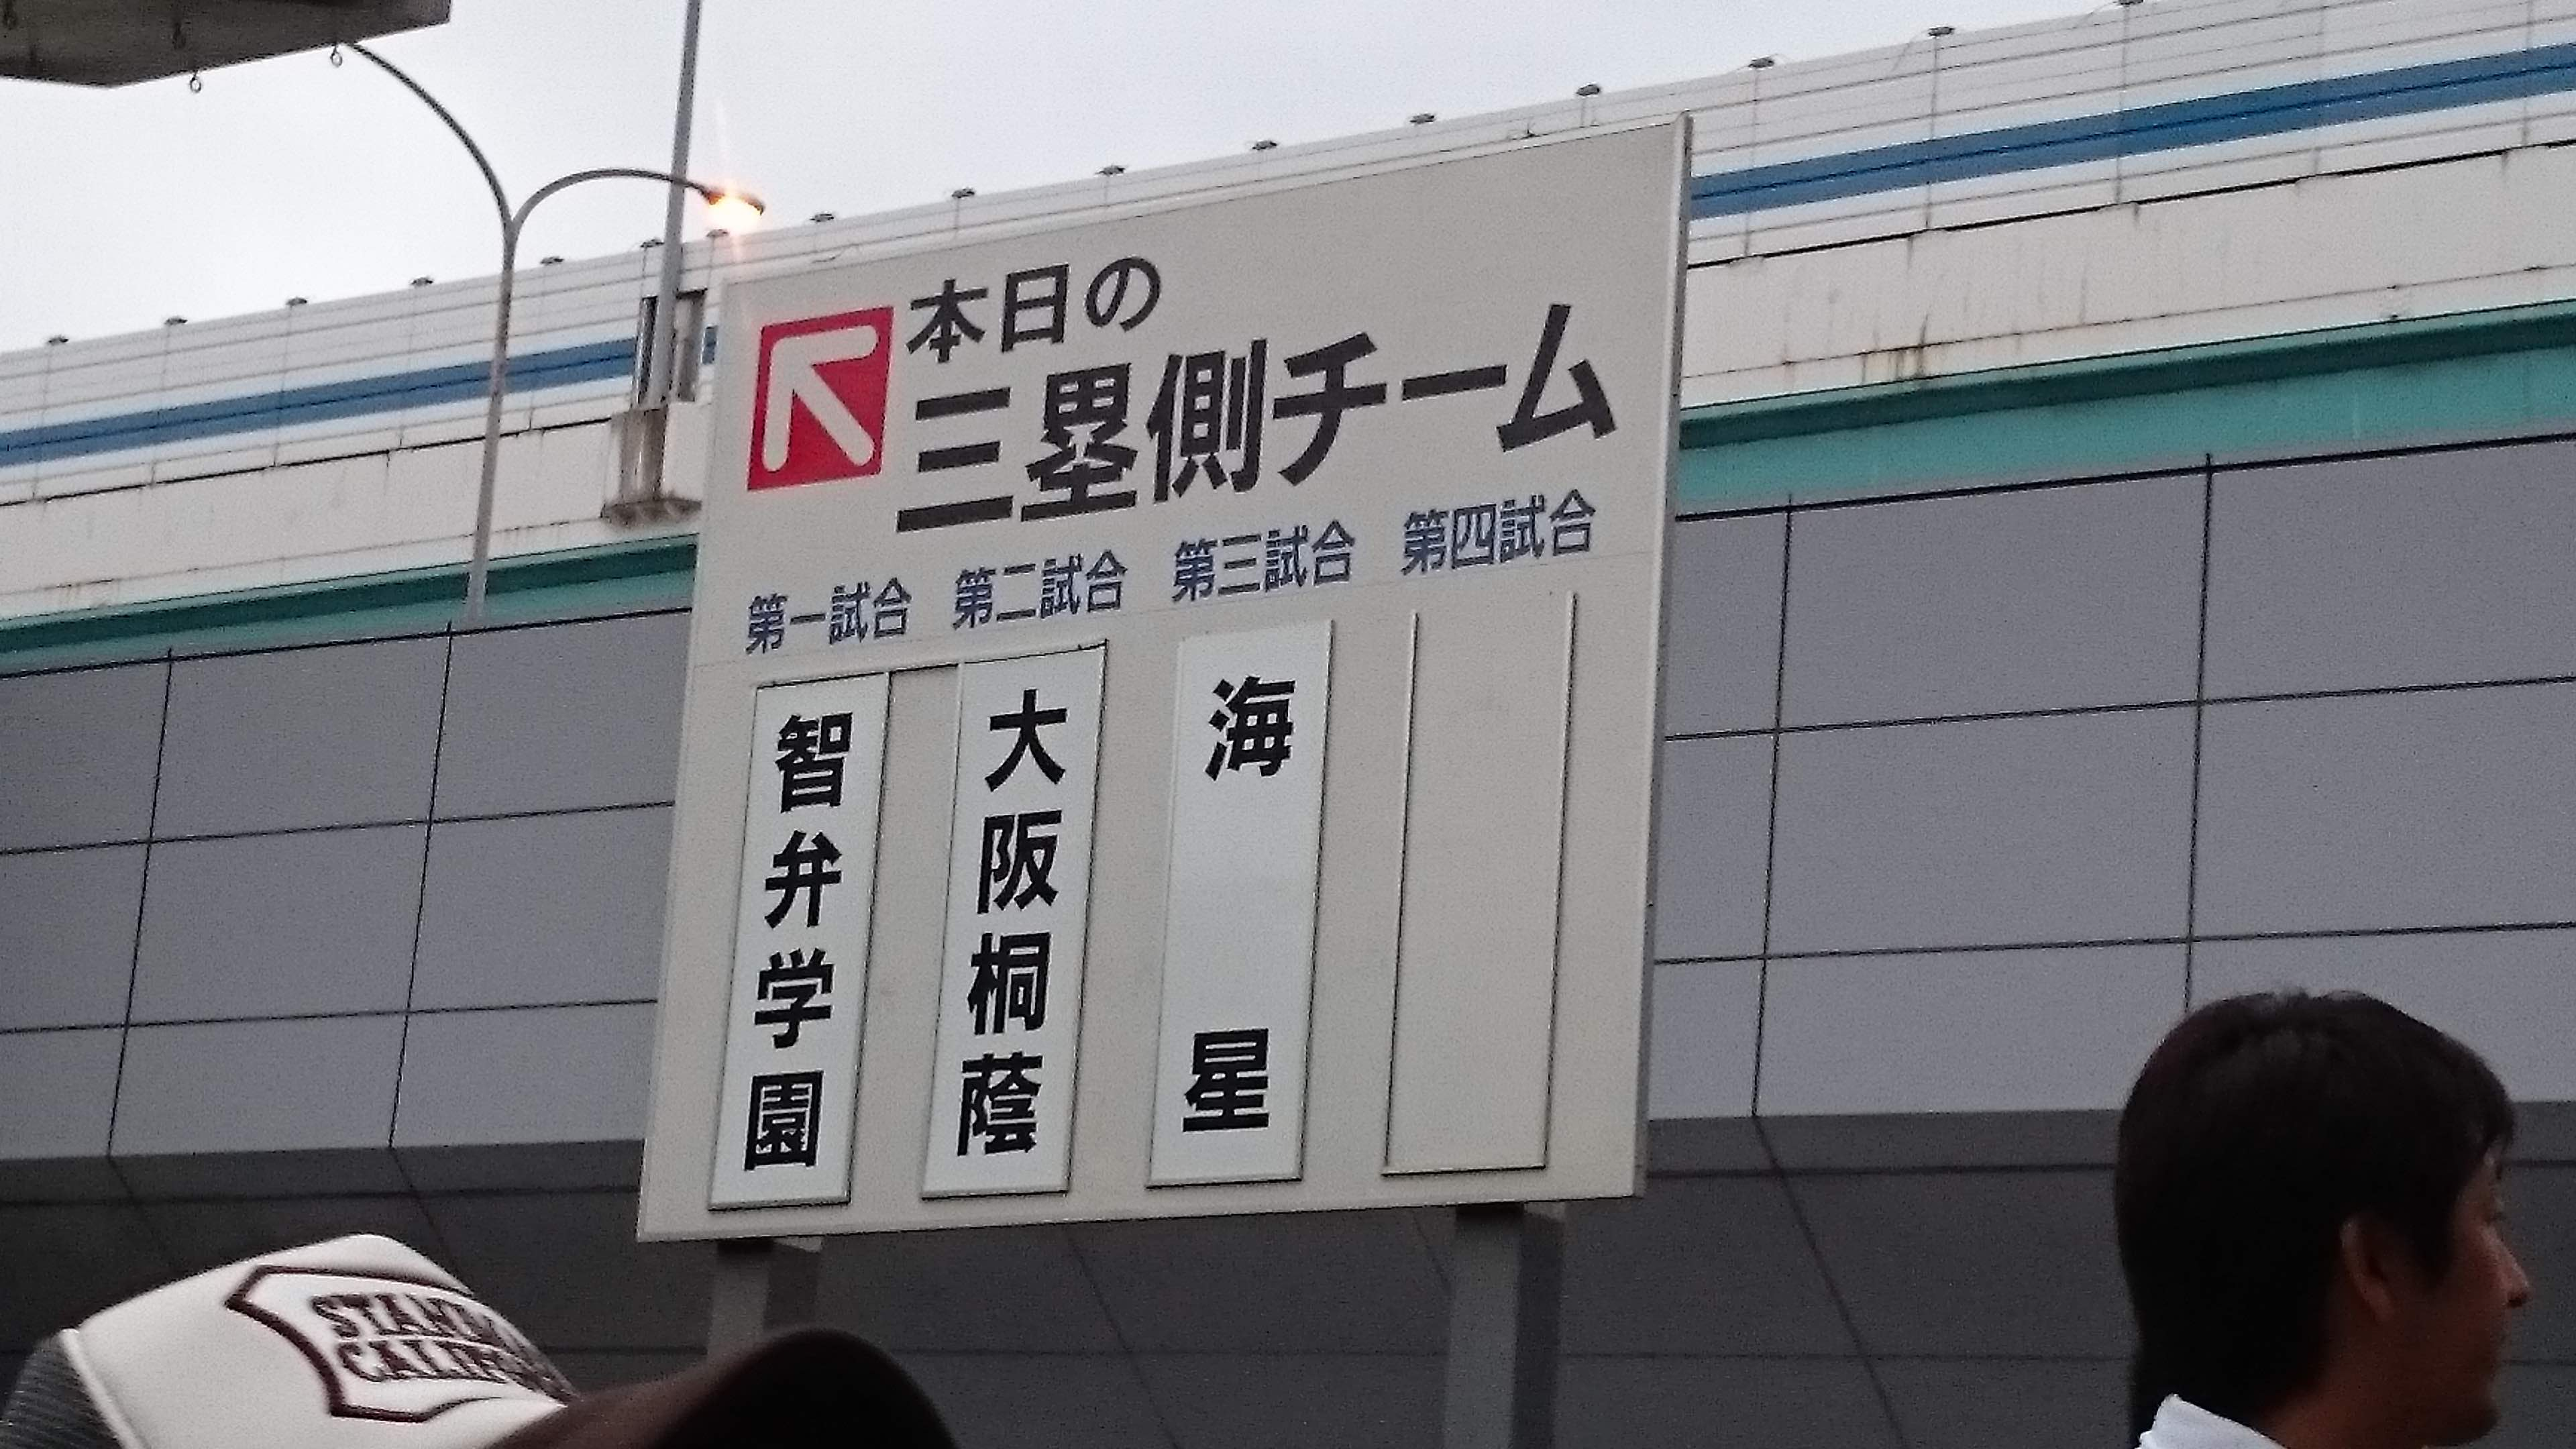
\includegraphics[width=0.7\textwidth]{./section/Shokuji/figures/Koushien_2.jpg}
  \caption{本日の三塁側のチーム}
\label{Fig:Seiza}
\end{figure}
% ----------------------------------------

% ----------------------------------------
\begin{figure}[h]
\centering
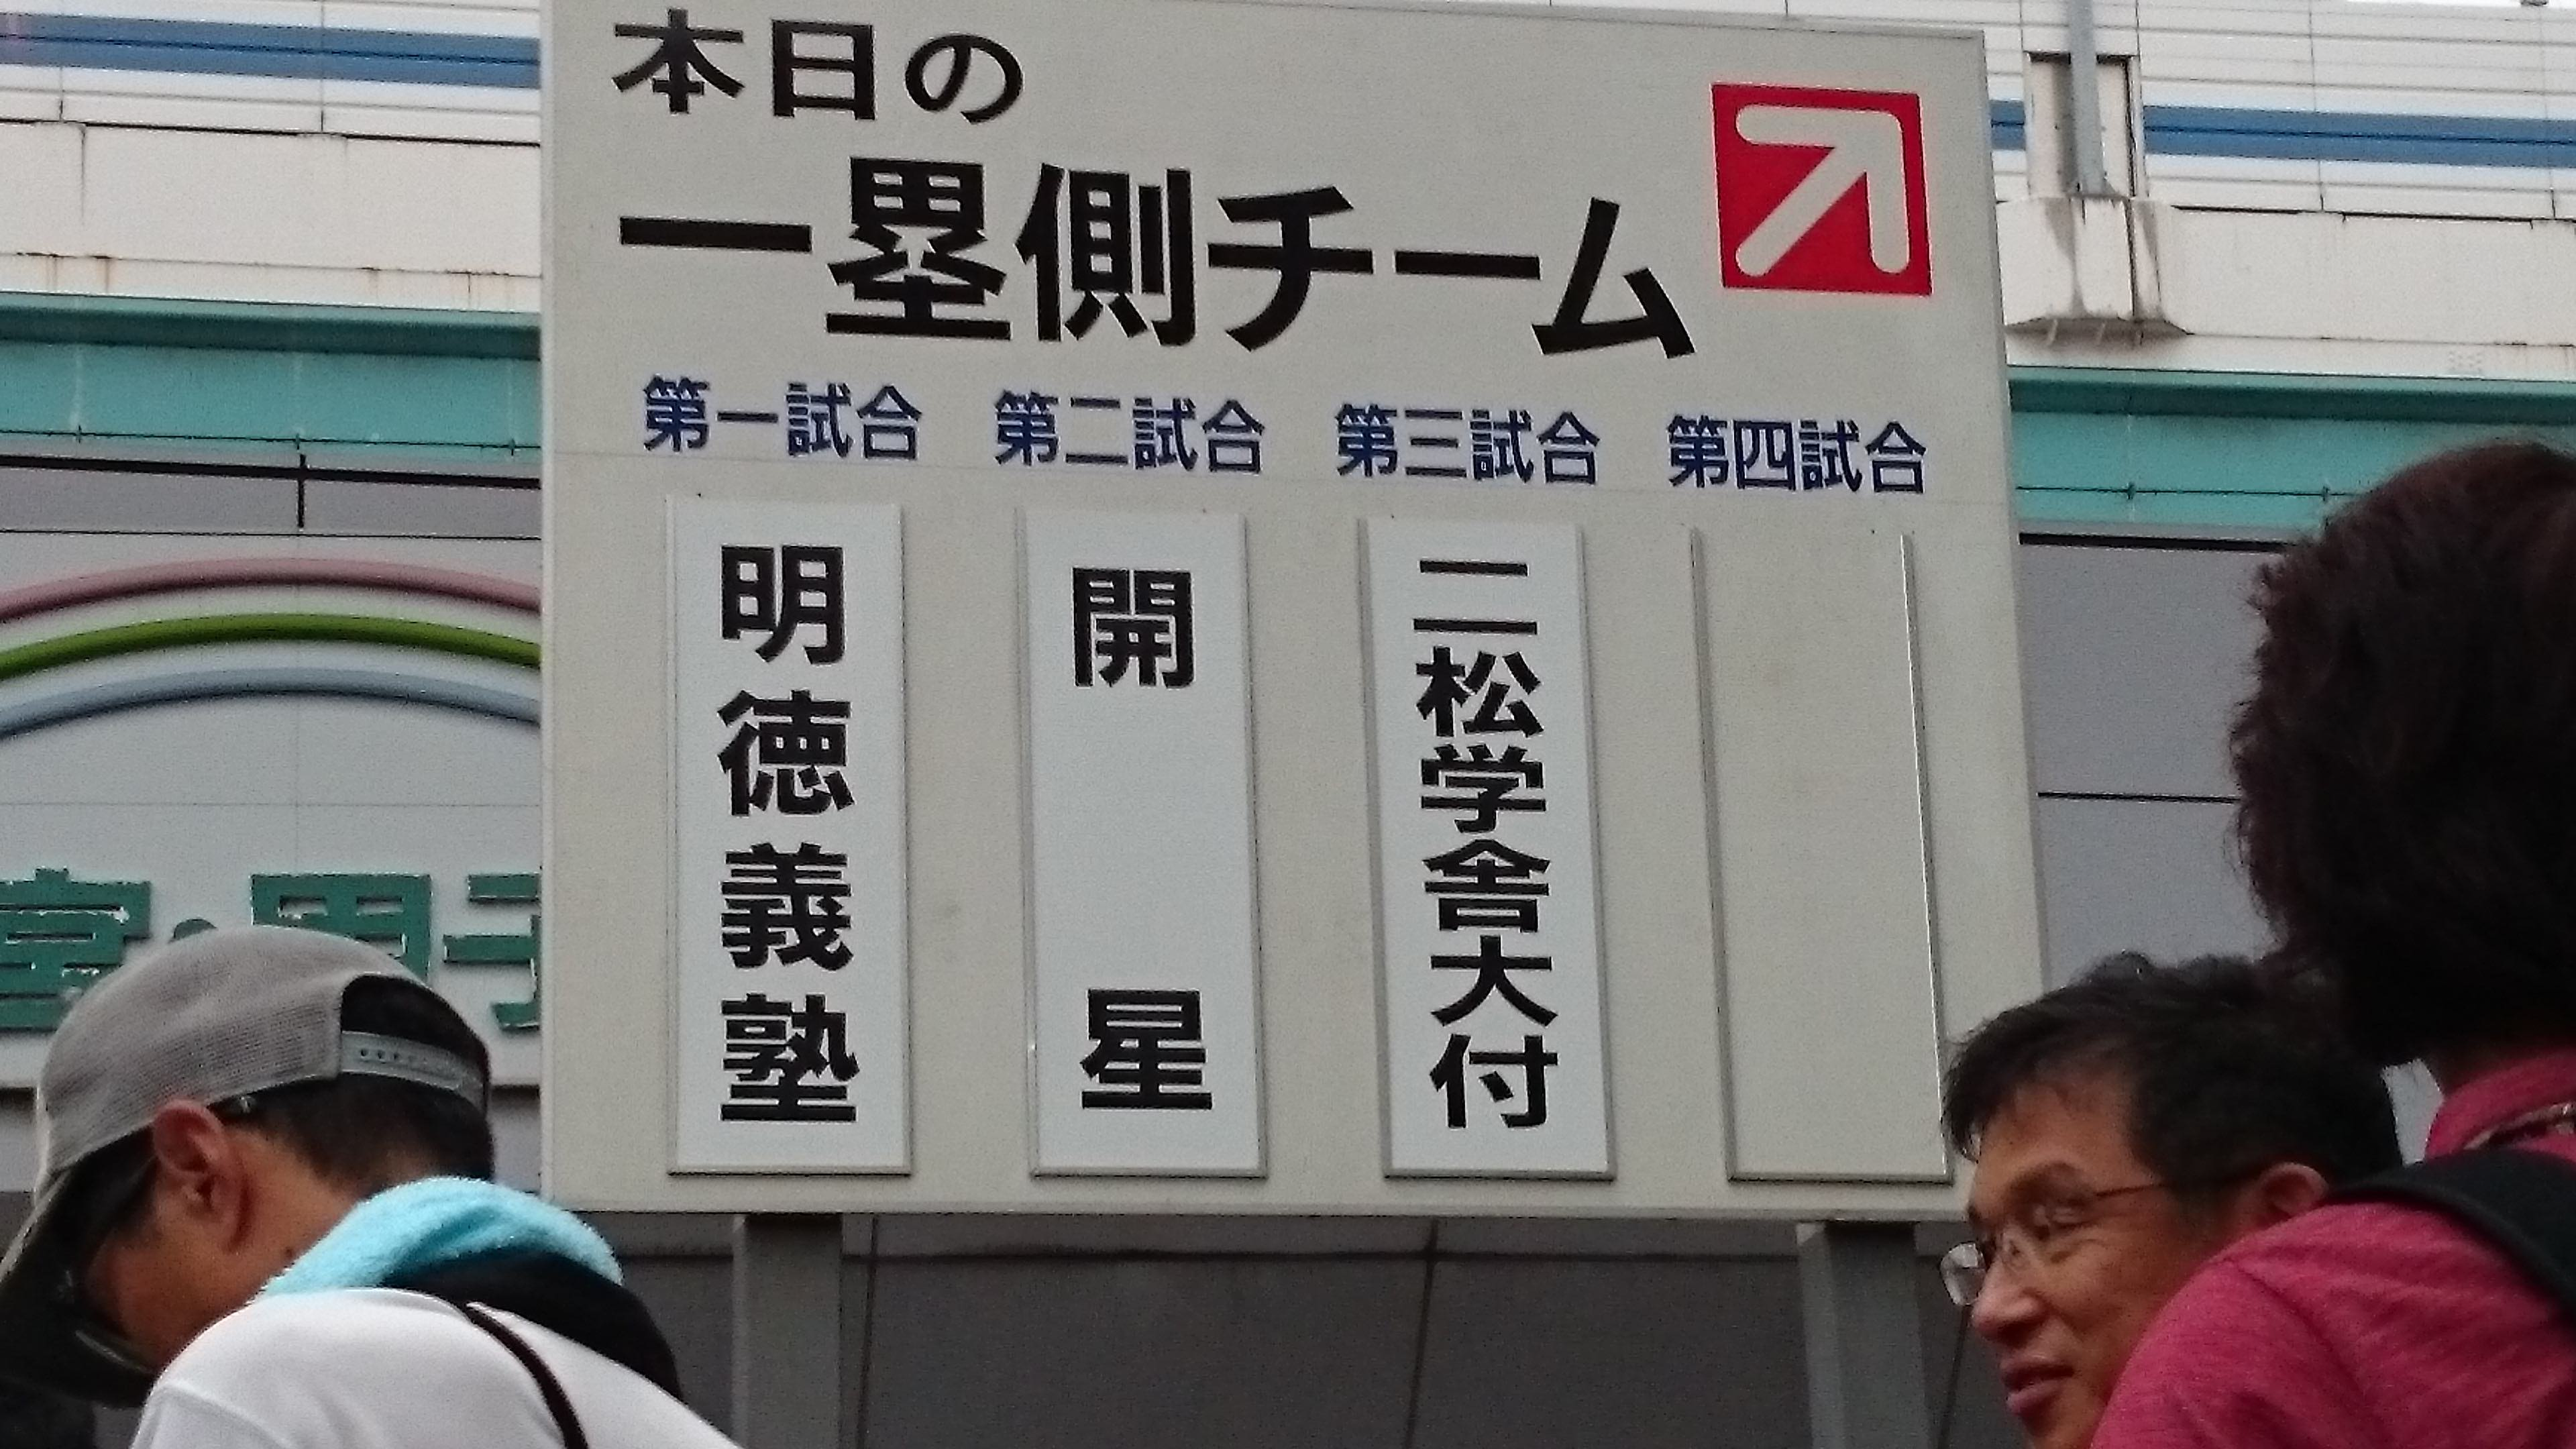
\includegraphics[width=0.7\textwidth]{./section/Shokuji/figures/Koushien_3.jpg}
  \caption{本日の一塁側のチーム}
\label{Fig:Seiza}
\end{figure}
% ----------------------------------------

\subsection{殴り込み}
いざ球場に入ると、感動もひとしお。しかし彼らの目的は、野球を楽しむことではなく、殴り込みに行くことであったので、オガワ氏は殴り込もうと思った。
その矢先、市民は恐れをなしてオガワ氏から逃げていくではないか!

% ----------------------------------------
\begin{figure}[h]
\centering
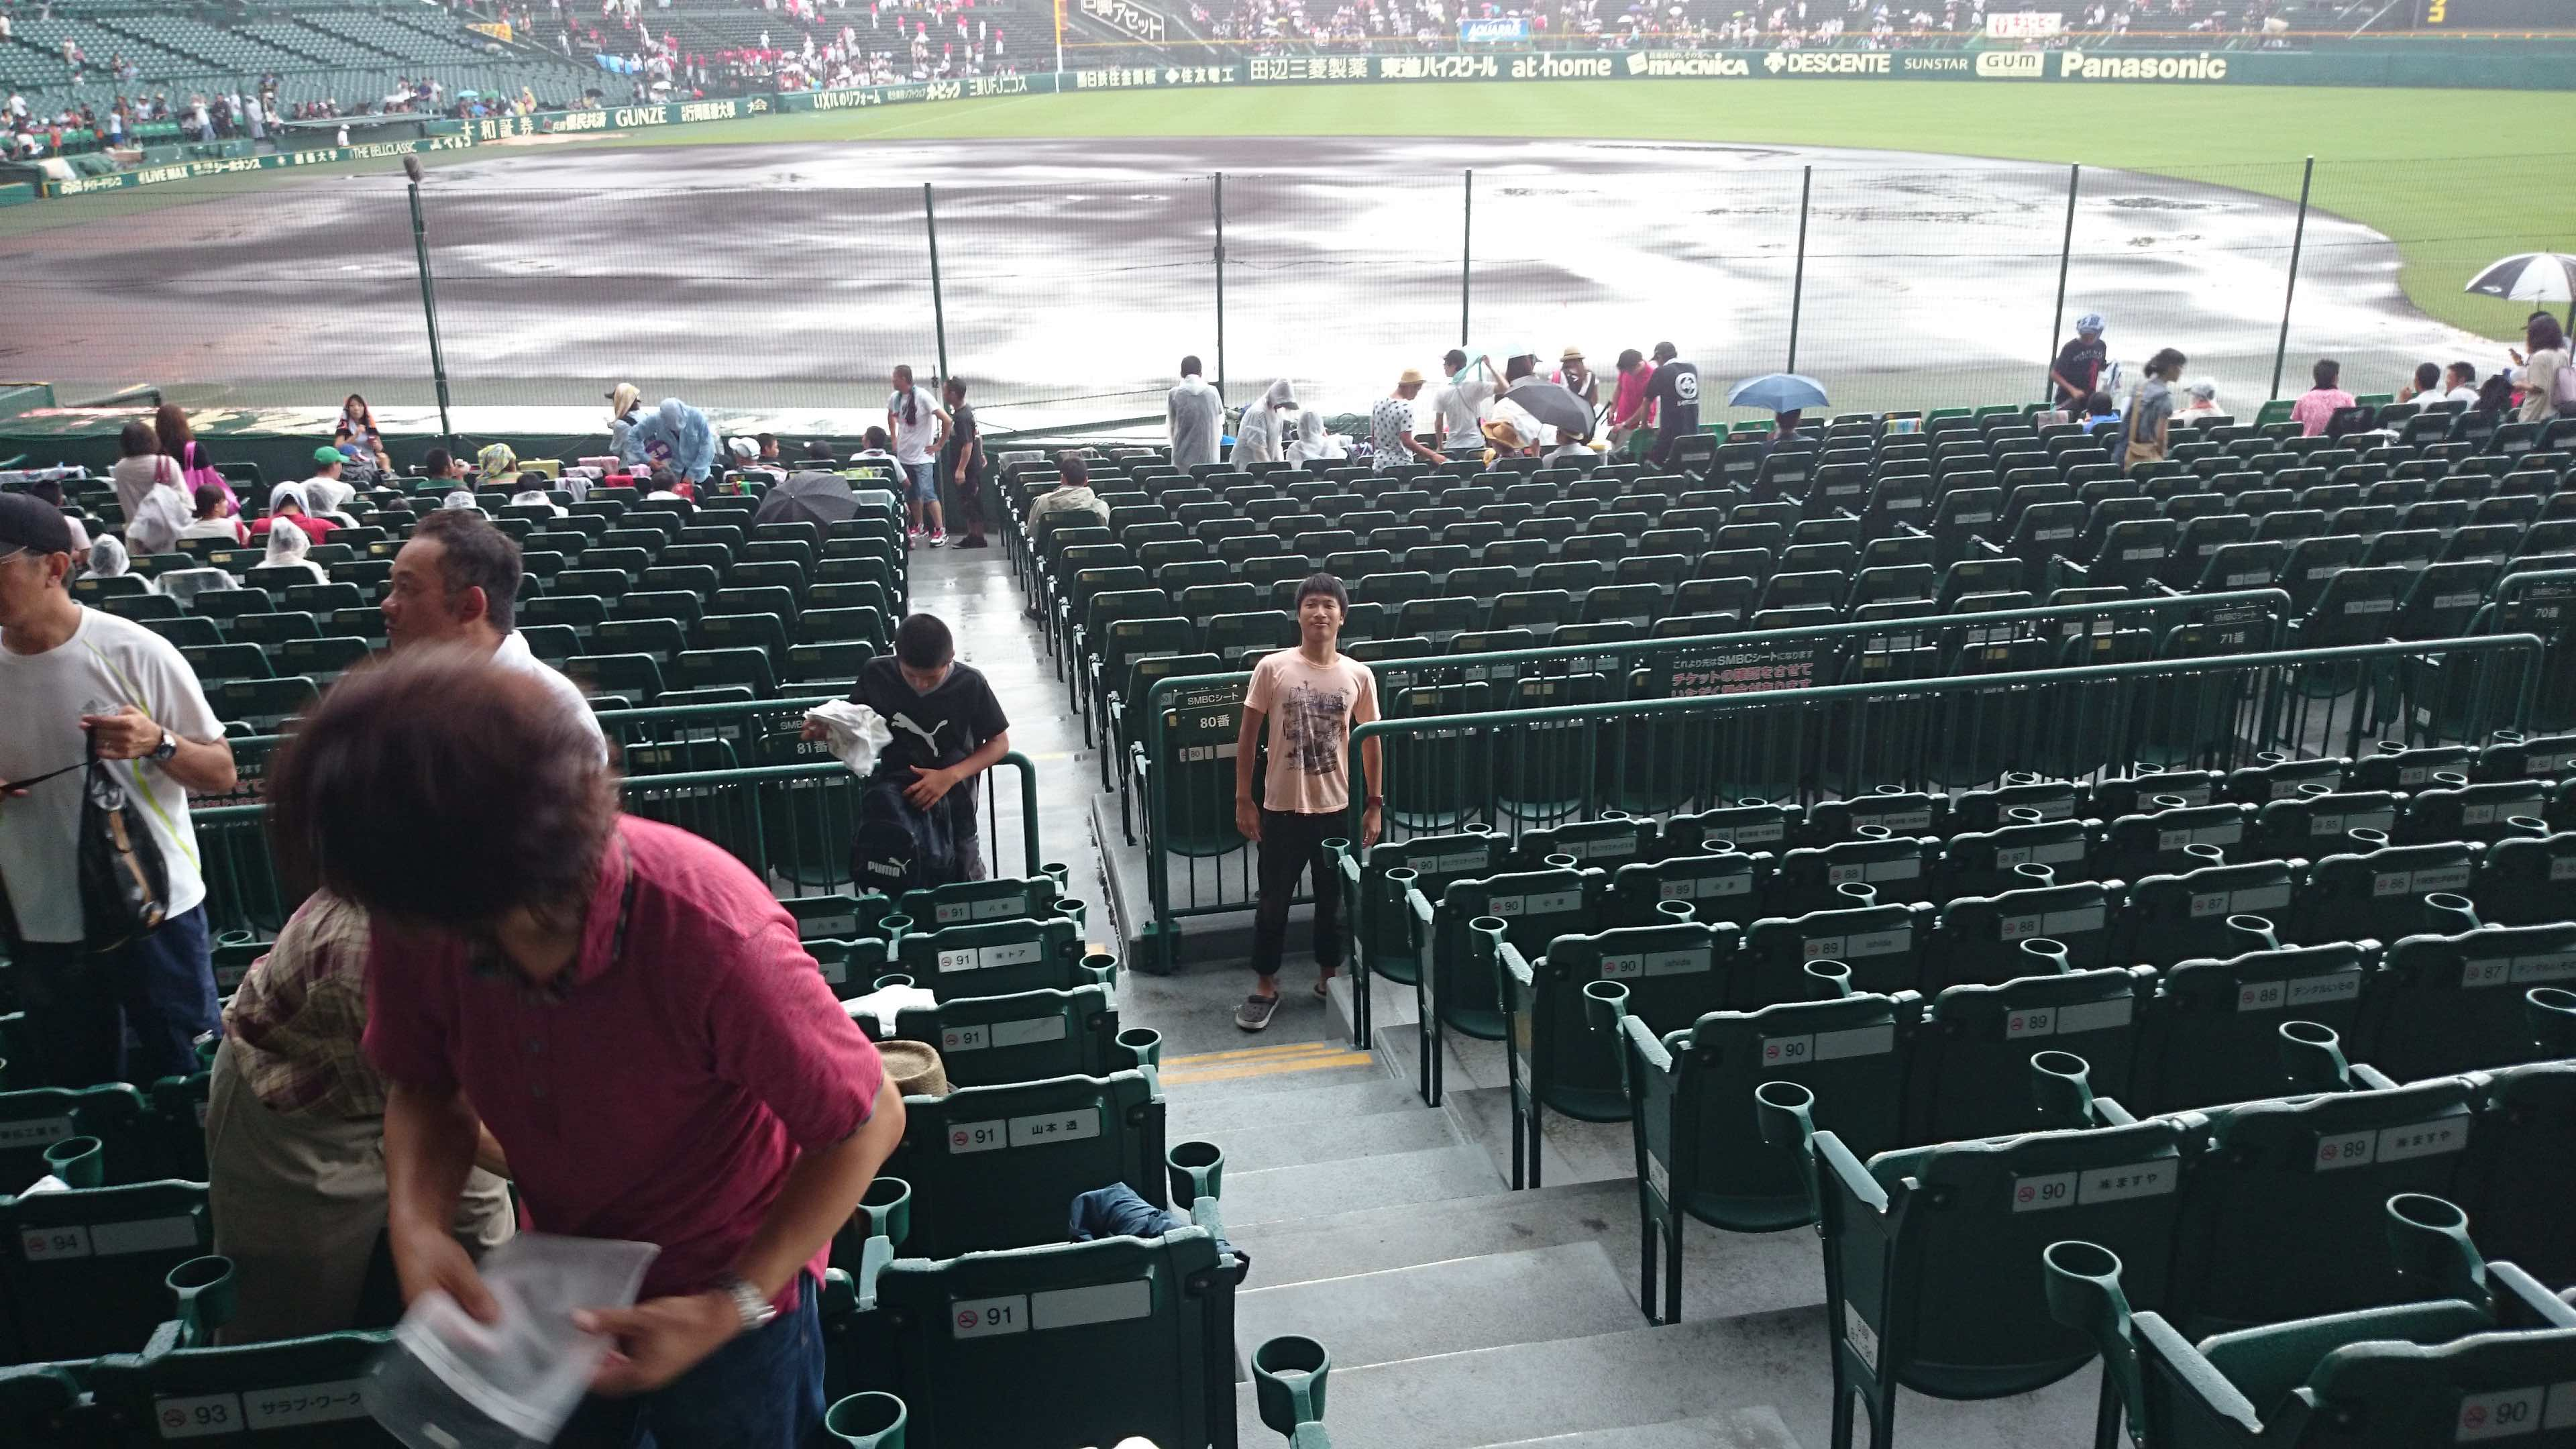
\includegraphics[width=0.7\textwidth]{./section/Shokuji/figures/Koushien_4.jpg}
  \caption{こちらを向き、たたずむ小川青年。}
\label{Fig:Seiza}
\end{figure}
% ----------------------------------------




%%%%%%%%%%%%%%%%%%%%%%%%%%%%%%%
\section{なんやこれ}
%%%%%%%%%%%%%%%%%%%%%%%%%%%%%%%
人生勝ち組の男が、こちらを睨んでいる。
武田学長の権力を持ってさえも、クビにすることはできない。
民主党政権時の、スーパーコンピューターの予算を削る時に、この男も削られればよかったのである。

% ----------------------------------------
\begin{figure}[h]
\centering
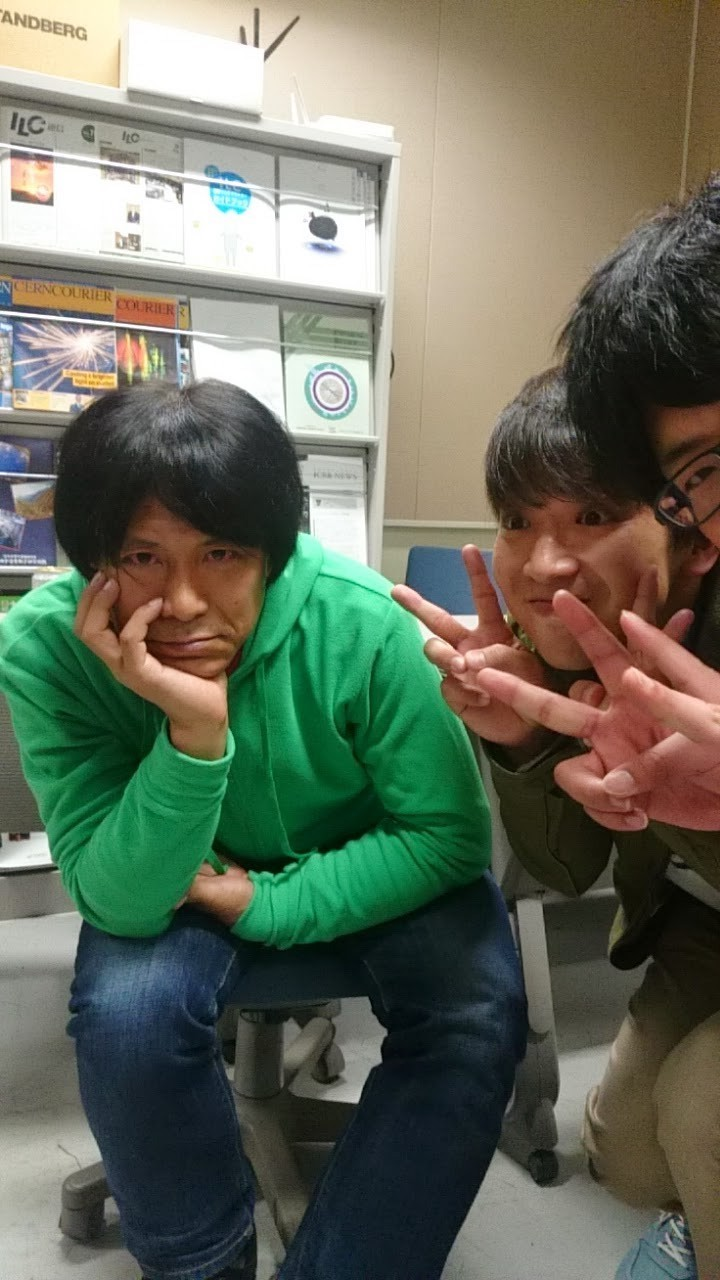
\includegraphics[width=0.4\textwidth]{./section/Shokuji/figures/Nanyakore.jpg}
  \caption{見方を変えれば人生勝ち組の助教授。床で寝てるだけで年収数百万円なのだから。}
\label{Fig:Seiza}
\end{figure}
% ----------------------------------------


\subsection{オガワ・バイク・オガワ(OBO)}
オガワは、学長に就任して以来、経営危機にあった非言語大学をV字回復させた。
さらに、ルノーや三菱自動車の会長も兼務した、世界的なカリスマ経営者として伝説に残っている。
このような経営改革を行ってきた、オガワ学長がどのような人生を送ってきたか、機構長の観点から簡単に紹介する。

\begin{figure}[h]
\centering
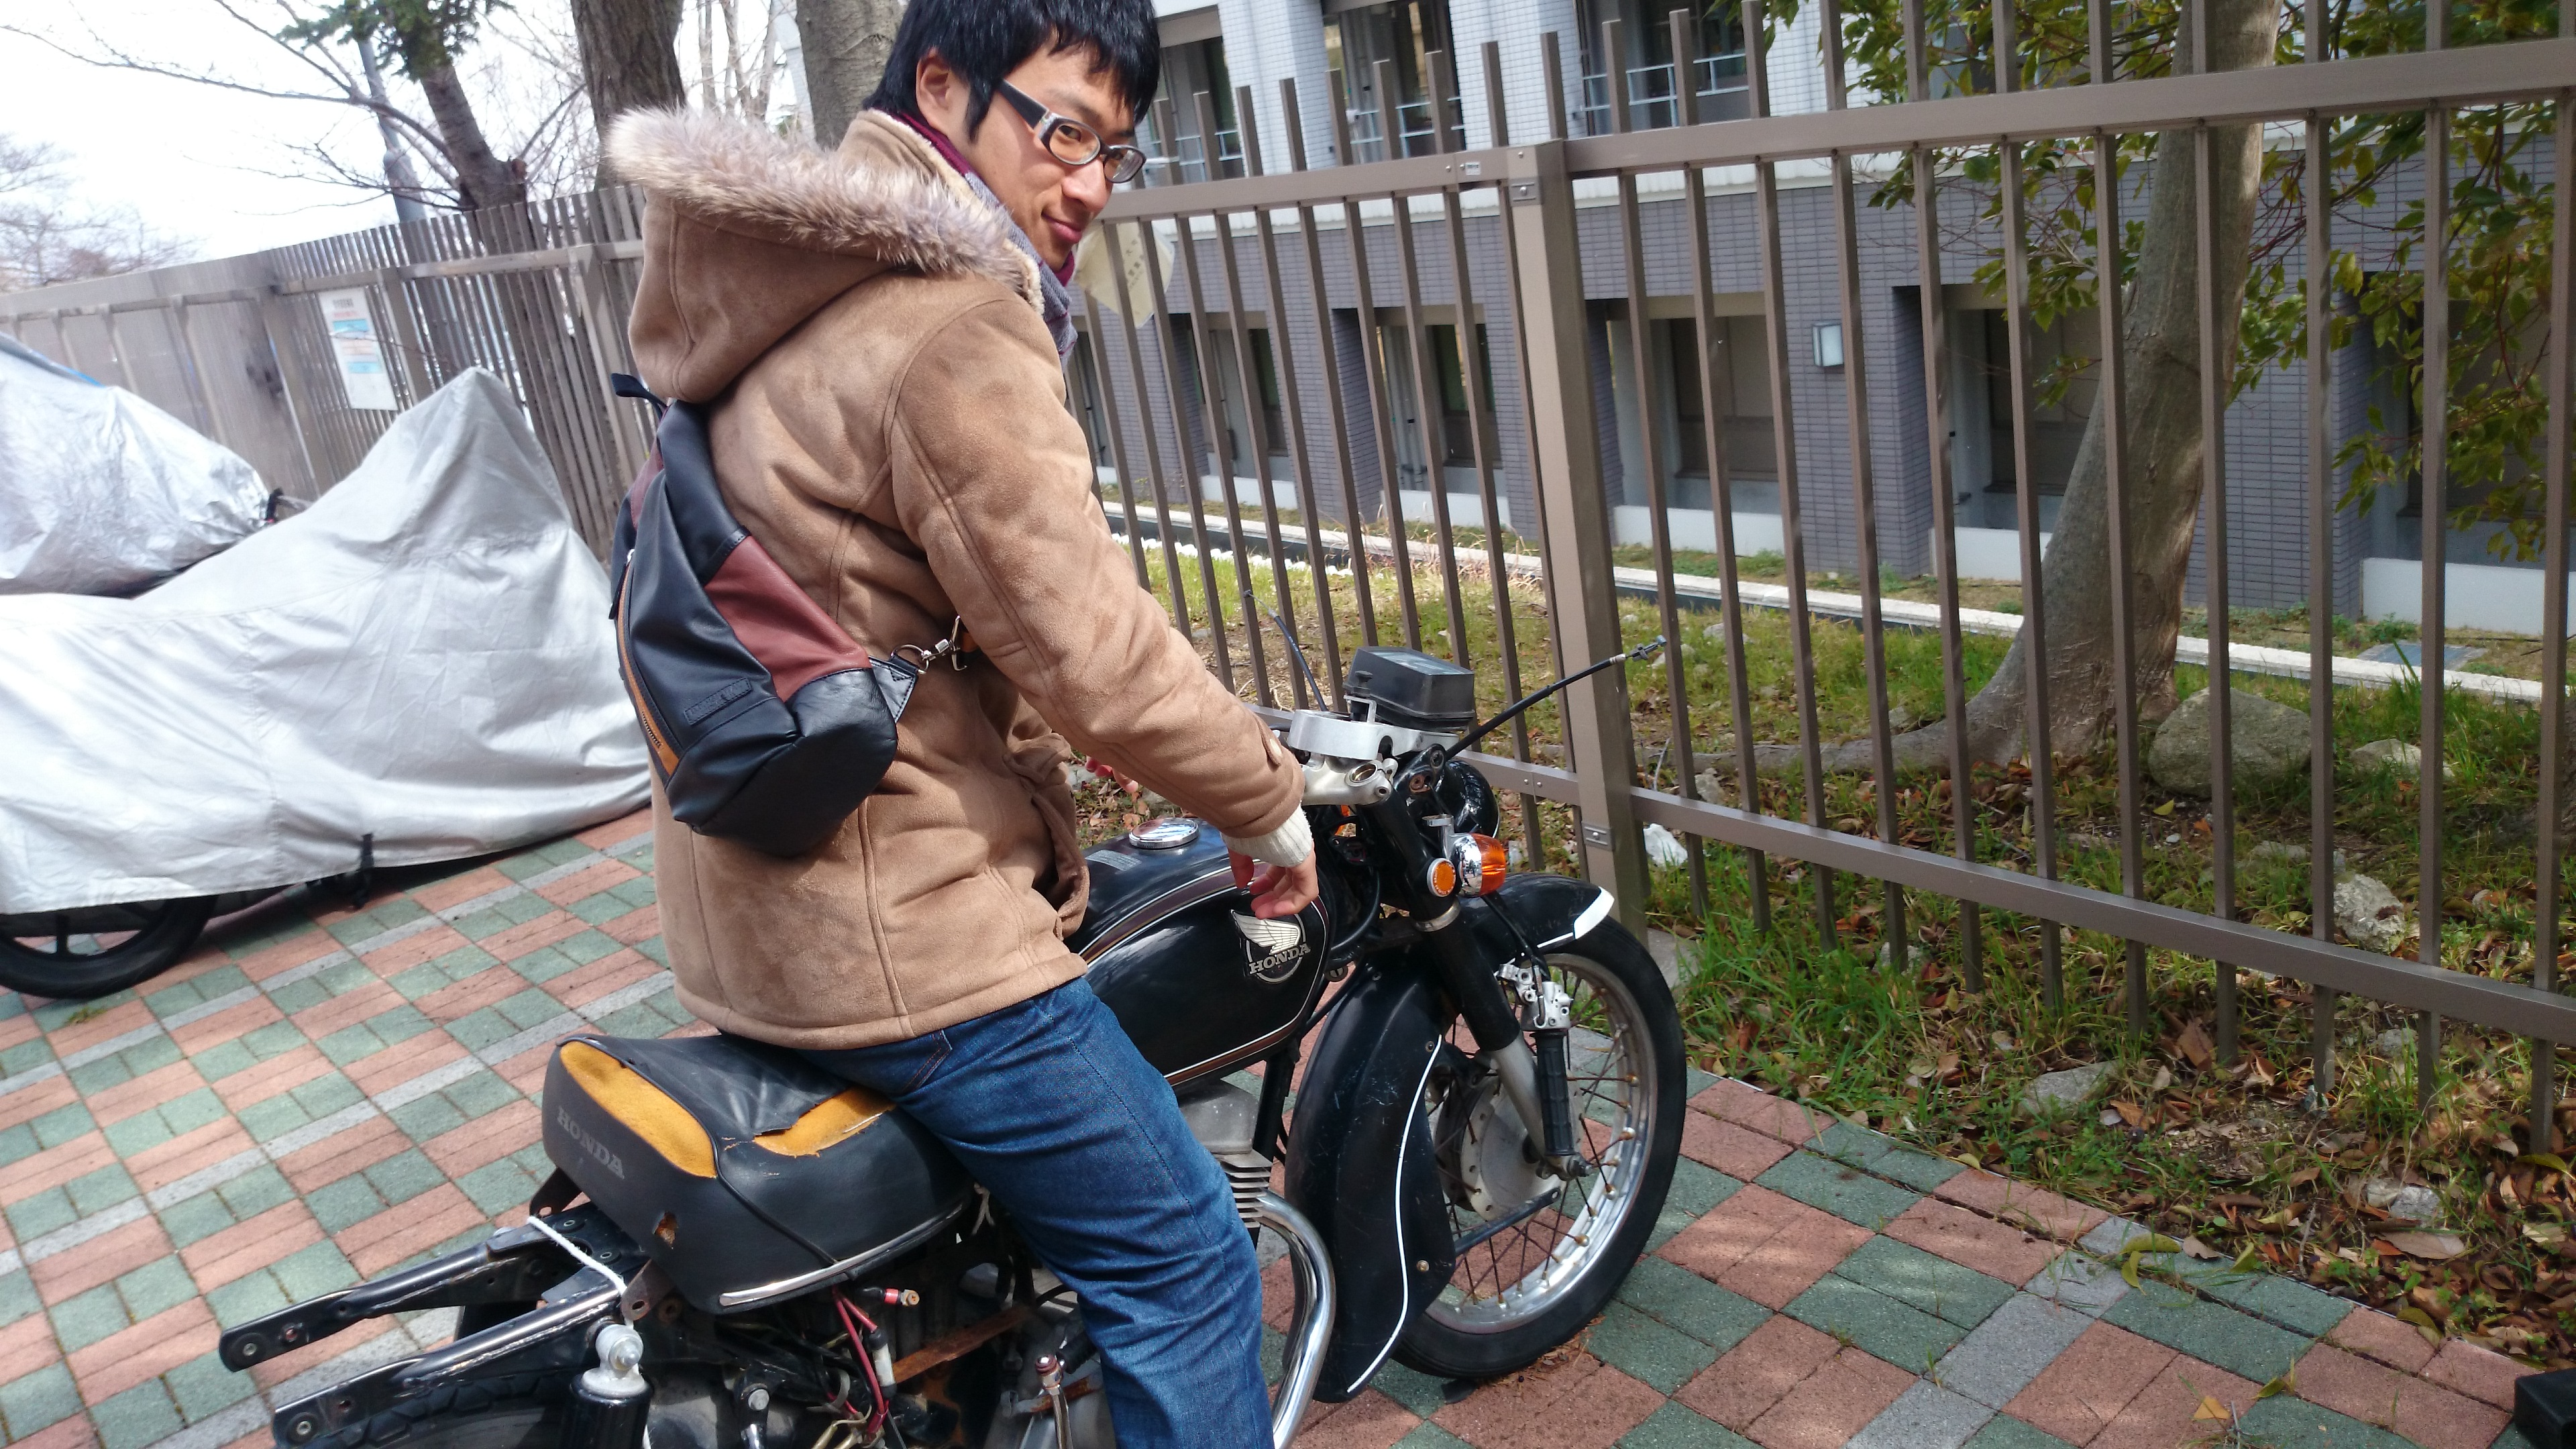
\includegraphics[width=0.8\textwidth]{./section/HigengoUniv/figures/DSC_0113_2.jpg}
\caption{盗んだバイクで走り出す。学長と言えど、犯罪はおかすし、バイクで転ぶ。}
\end{figure}


%記憶の最初は、ヨネヨネCLUB創設である。
%阪急電車十三駅で特急に乗り換えているときに「Wikipediaでリンクを辿っていけば絶対に自分の行きたいページにいける」というネタをひっさげてお互い喋っていた。
%そのときに初代機構長が「こういうネタあるよ、小川くんの好きなものはなに?」という答えに対し「EXILE」であると答えたことが未だに記憶に残っている。
%案の定、任意のページからEXILEに辿り着き、まぁまぁ初対面ながら間がもったのは覚えている。



%%========================%
%\subsection{LIFE的観点}
%%========================%
%\begin{figure}
%\centering
%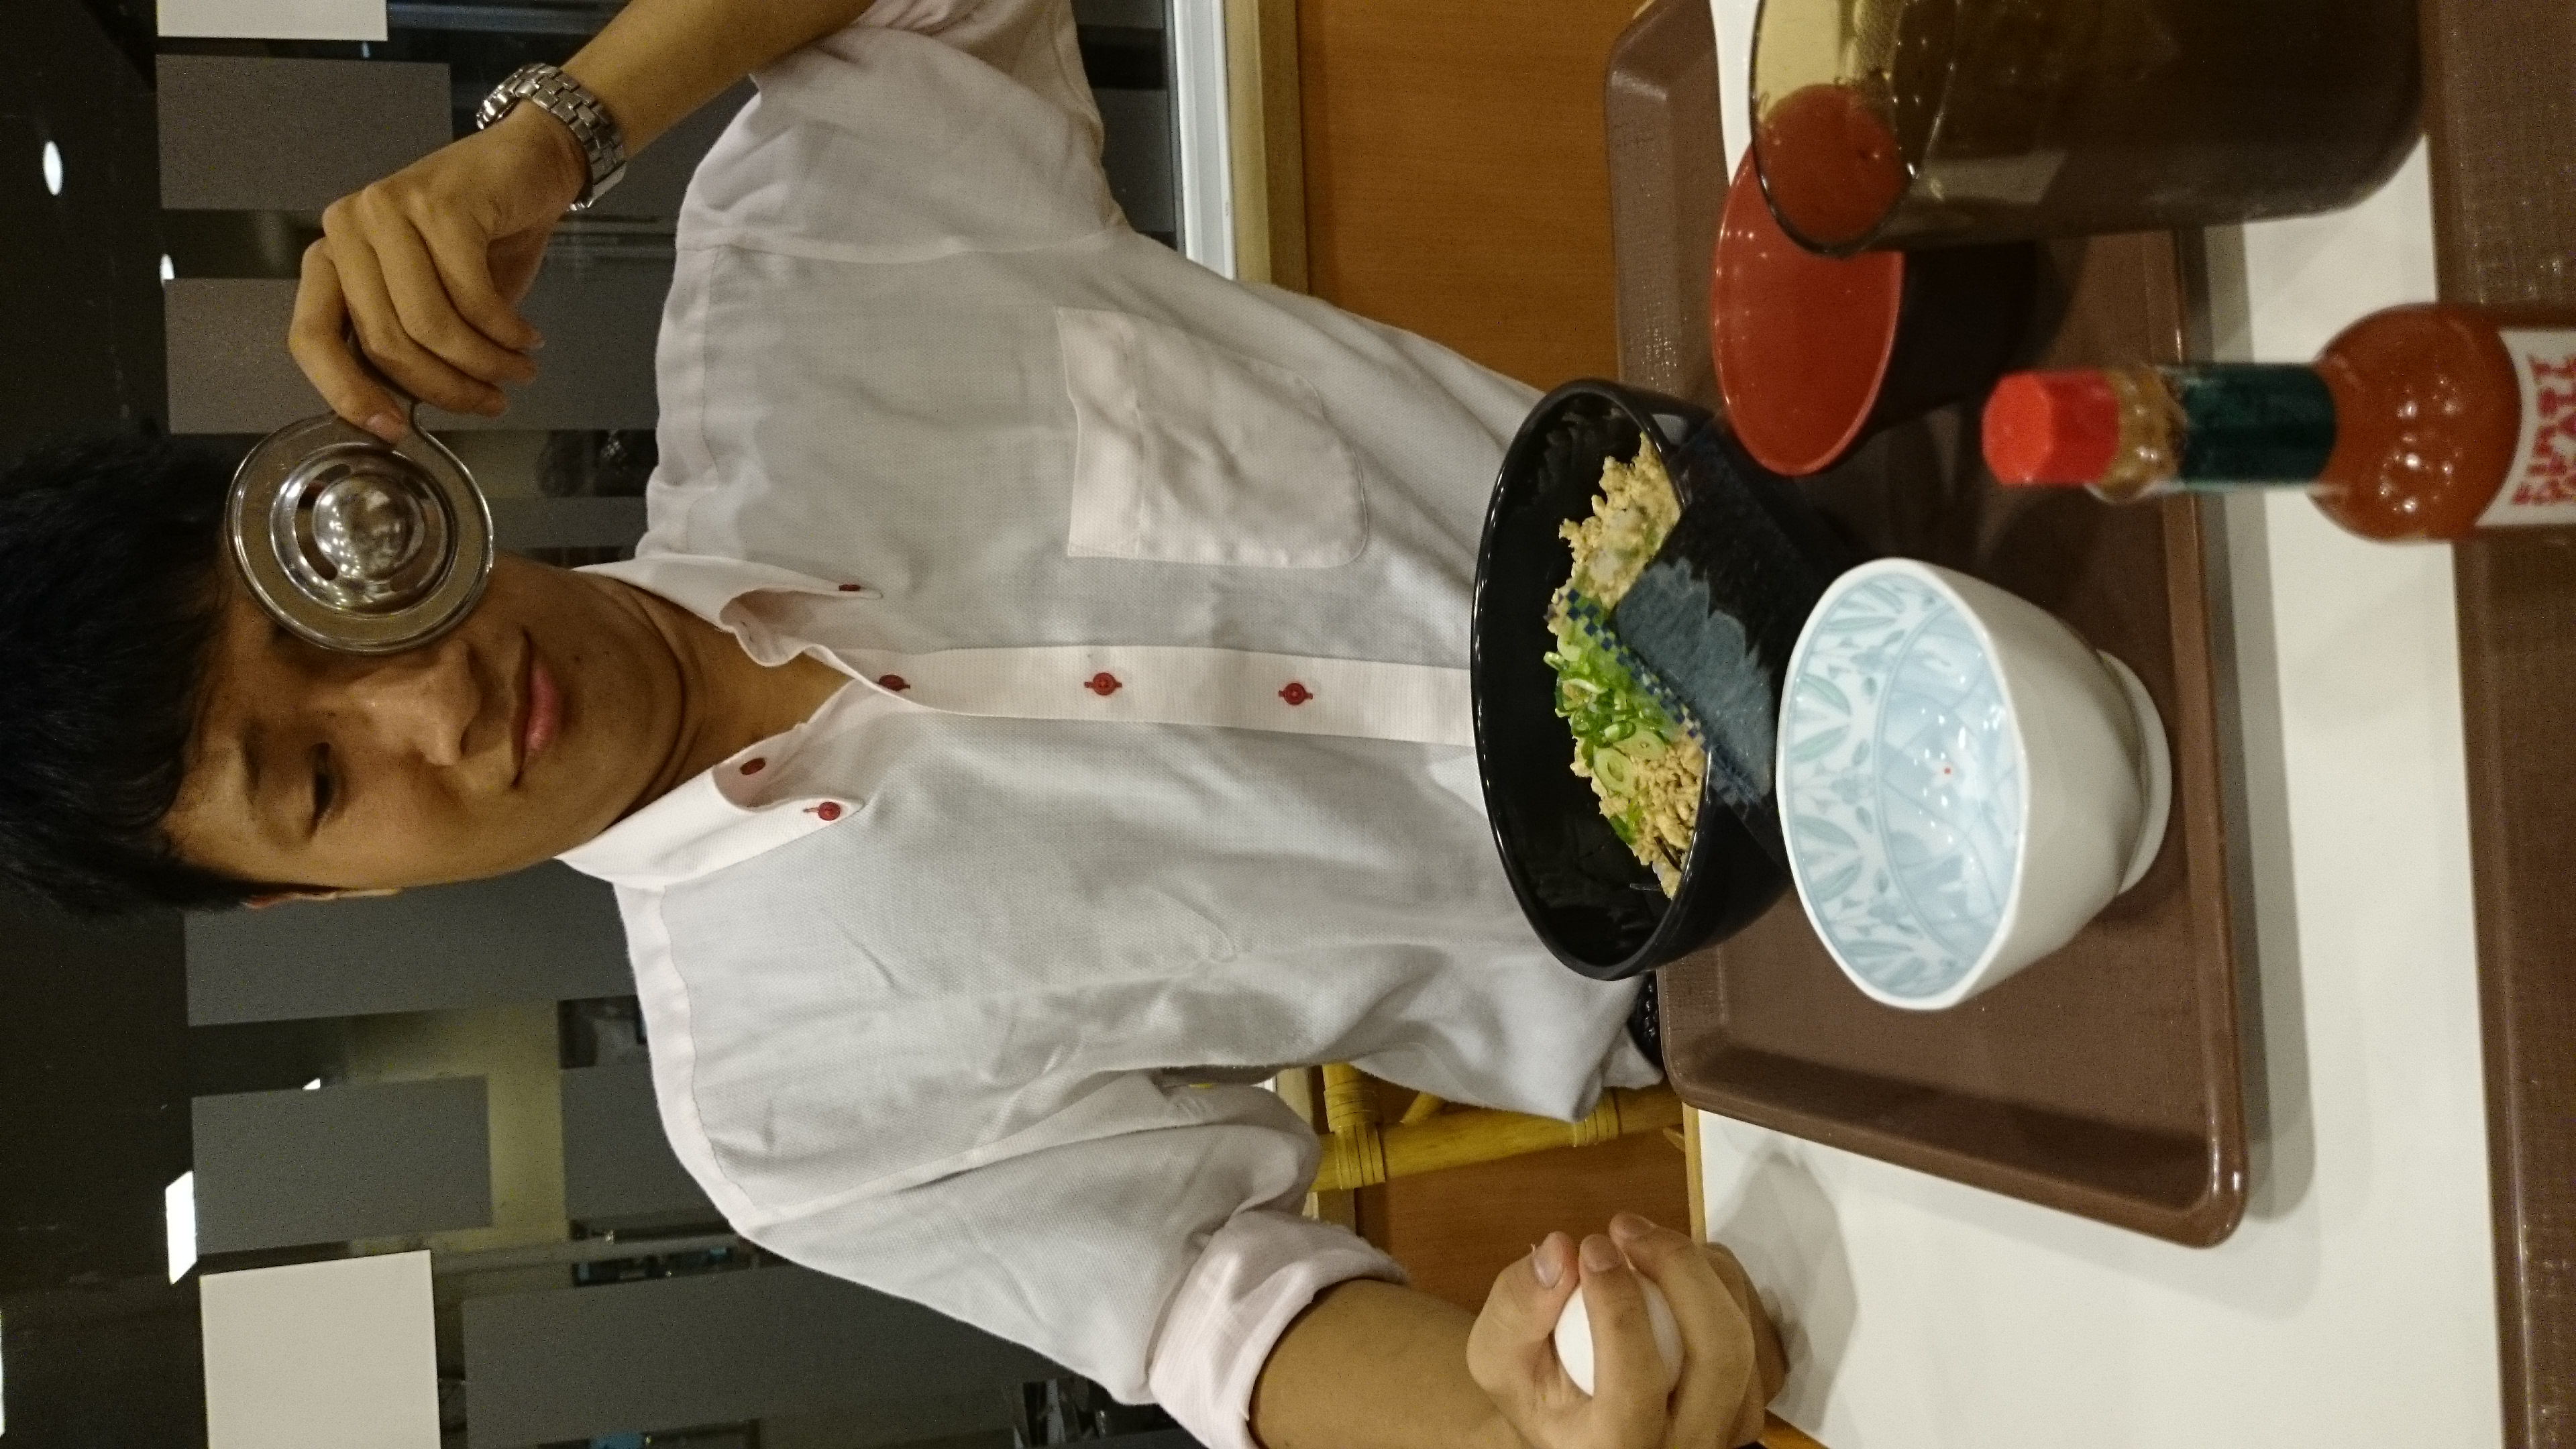
\includegraphics[scale=0.1]{./section/HigengoUniv/figures/DebuKatsu.jpg}
%\caption{ライフ近くの晩ごはん屋さん。}
%\label{mimi}
%\end{figure}


%学部生3回生の頃の初代機構長はバイト先に困っていた。
%そのところに、小川総務大臣の助言によりライフで働くことになった。なんとなくレジに興味あると言って、なんとなくレジ部門になった。半額ボタンを押して色々買ったり、買い物に来た宮崎大輔のコメを半額にしてやった。ある程度してやめた。
%ここから俗に言うデブ活が更に加速していったのである。



%\subsection{建立(ケンリツ)}
%非言語革命により設立された非言語大学であるが、特に初代機構長は様々な新歓を渡り歩き、初代総務大臣はCSC(?)を渡り歩いていた。






